%%%%%%%%%%%%%%%%%%%%%%%%%%%%%%%%%%%%%%%%%
% University Assignment Title Page 
% LaTeX Template
% Version 1.0 (27/12/12)
%
% This template has been downloaded from:
% http://www.LaTeXTemplates.com
%
% Original author:
% WikiBooks (http://en.wikibooks.org/wiki/LaTeX/Title_Creation)
%
% License:
% CC BY-NC-SA 3.0 (http://creativecommons.org/licenses/by-nc-sa/3.0/)
%
%%%%%%%%%%%%%%%%%%%%%%%%%%%%%%%%%%%%%%%%%
%\title{Title page with logo}
%----------------------------------------------------------------------------------------
%	PACKAGES AND OTHER DOCUMENT CONFIGURATIONS
%----------------------------------------------------------------------------------------

\documentclass[12pt]{article}
\usepackage[english]{babel}
\usepackage[utf8x]{inputenc}
\usepackage{natbib}
\usepackage[fleqn]{amsmath}
\usepackage{graphicx}
\usepackage[colorinlistoftodos]{todonotes}
\usepackage{listings}
\usepackage{color}
\usepackage[explicit]{titlesec}
\usepackage{url}


\definecolor{dkgreen}{rgb}{0,0.6,0}
\definecolor{gray}{rgb}{0.5,0.5,0.5}
\definecolor{mauve}{rgb}{0.58,0,0.82}

\begin{document}

\begin{titlepage}

\newcommand{\HRule}{\rule{\linewidth}{0.5mm}} % Defines a new command for the horizontal lines, change thickness here

\center % Center everything on the page
 
%----------------------------------------------------------------------------------------
%	HEADING SECTIONS
%----------------------------------------------------------------------------------------

\textsc{\LARGE University of St Andrews}\\[1.5cm] % Name of your university/college
\textsc{\Large CS4302 Practical 3}\\[0.5cm] % Major heading such as course name
\textsc{\large }\\[0.5cm] % Minor heading such as course title

%----------------------------------------------------------------------------------------
%	TITLE SECTION
%----------------------------------------------------------------------------------------

\HRule \\[0.4cm]
{ \huge \bfseries Image Processing}\\[0.4cm] % Title of your document
\HRule \\[1.5cm]
 
%----------------------------------------------------------------------------------------
%	AUTHOR SECTION
%----------------------------------------------------------------------------------------


\Large \emph{Author:}\\
 \textsc{150008022}\\[3cm] % Your name

%----------------------------------------------------------------------------------------
%	DATE SECTION
%----------------------------------------------------------------------------------------

{\large \today}\\[2cm] % Date, change the \today to a set date if you want to be precise

%----------------------------------------------------------------------------------------
%	LOGO SECTION
%---------------------------------------------------------------------------------------


\includegraphics[width = 3.1cm]{images/standrewslogo.png}
 
%----------------------------------------------------------------------------------------

\vfill % Fill the rest of the page with whitespace

\end{titlepage}

\part*{Goal}

The goal of this practical was to learn and apply image processing techniques using Matlab\textsuperscript{\textregistered}.

\part*{Tasks}

The scripts are separated by task given in the practical specification. Where useful, scripts were created to hold functions that were used repeatedly. To run each practical task in order, the script \emph{practical.m} can be used (This will generate a large number of figures). The images for processing are shown in figures \ref{fig:colorful}, \ref{fig:drawing}, and \ref{fig:simple}.

\begin{figure}[h]
  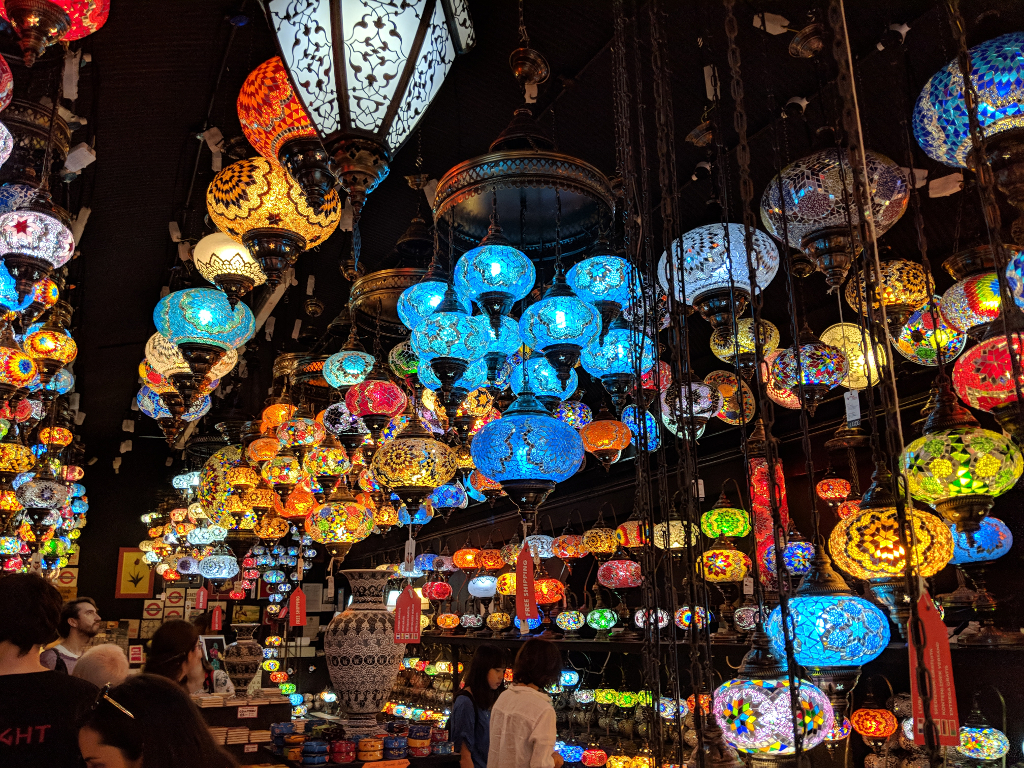
\includegraphics[width=\linewidth]{images/colourful.jpg}
  \caption{Image with large variation in colour and spatial frequency.}
  \label{fig:colorful}
\end{figure}

\begin{figure}[ht]
  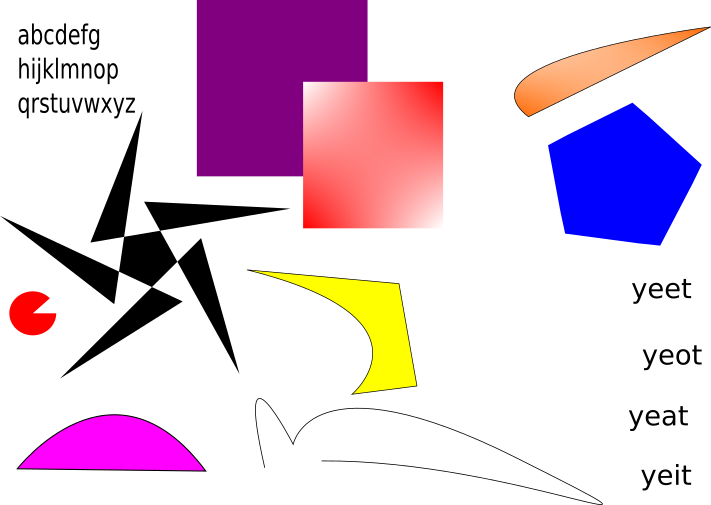
\includegraphics[width=\linewidth]{images/drawing.png}
  \caption{Vector image featuring text, polygons, and bezier curves. Originally created in Inkscape and exported as a PNG file.}
  \label{fig:drawing}
\end{figure}
  
\begin{figure}[hb]
  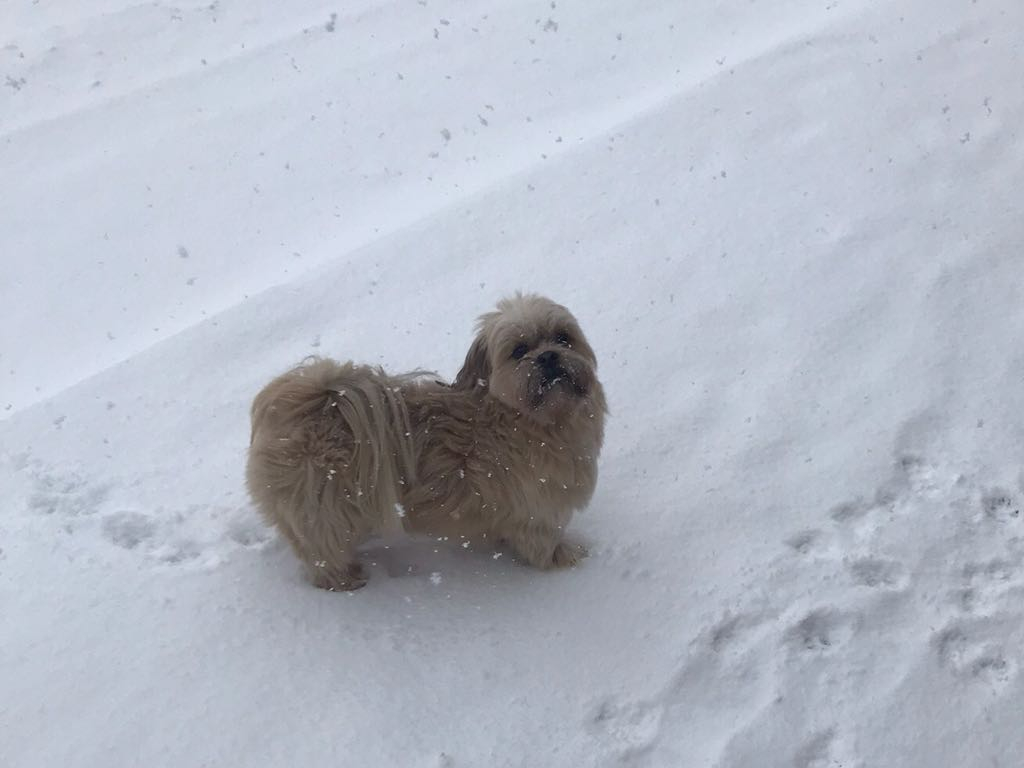
\includegraphics[width=\linewidth]{images/simple.jpg}
  \caption{Simple image with little variation in colour or spatial frequency.}
  \label{fig:simple}
\end{figure}

\vfill
\clearpage

\section{RGB}

For task 1, the function \emph{showRGB.m} was created. After reading the files using \emph{imread}, the three colour planes were seperated. These were then all plotted individually for each image file. Since each colour has 256 values (given 8 bits each), the colourbar was supplied the range 0 to 256. 

Figure \ref{fig:colorful} was filtered into figures \ref{fig:colourfulred}, \ref{fig:colourfulgreen}, and \ref{fig:colourfulblue}. Lanterns in the image that are most saturated are replaced with black in all other colour filtered images. For example, the blue lanterns roughly in the centre of the blue channel image are not visible in the red channel image. Since white is composed of all three colours, the white circles in the centre of the blue lanterns is still visible in each image. A similar effect can be seen in each of the other images. 

\begin{figure}[h]
  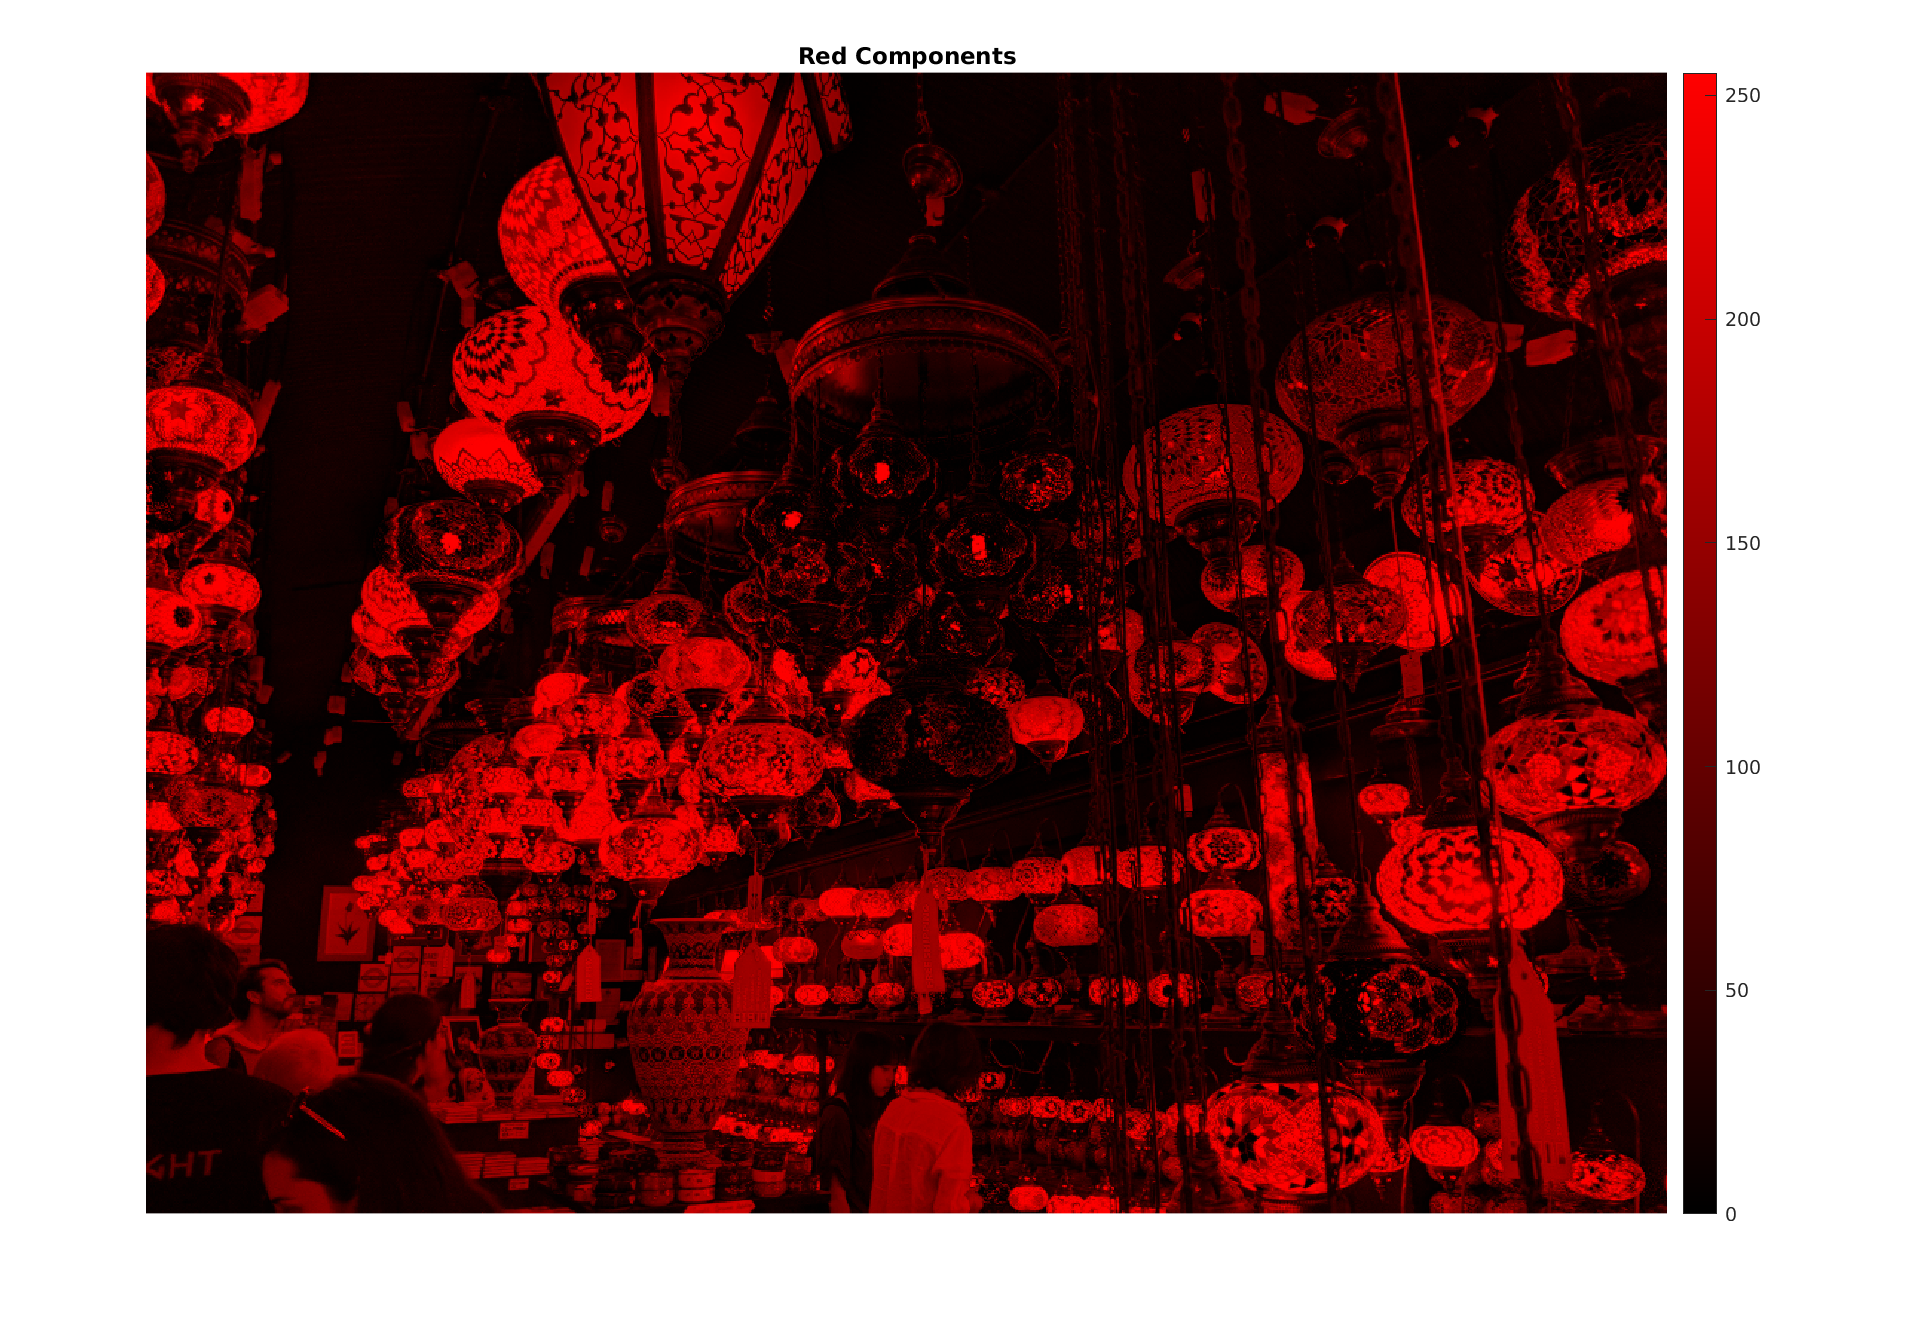
\includegraphics[width=\linewidth]{images/task1/colourfulr.png}
  \caption{Red component of Figure \ref{fig:colorful}.}
  \label{fig:colourfulred}
\end{figure}

\begin{figure}[h]
  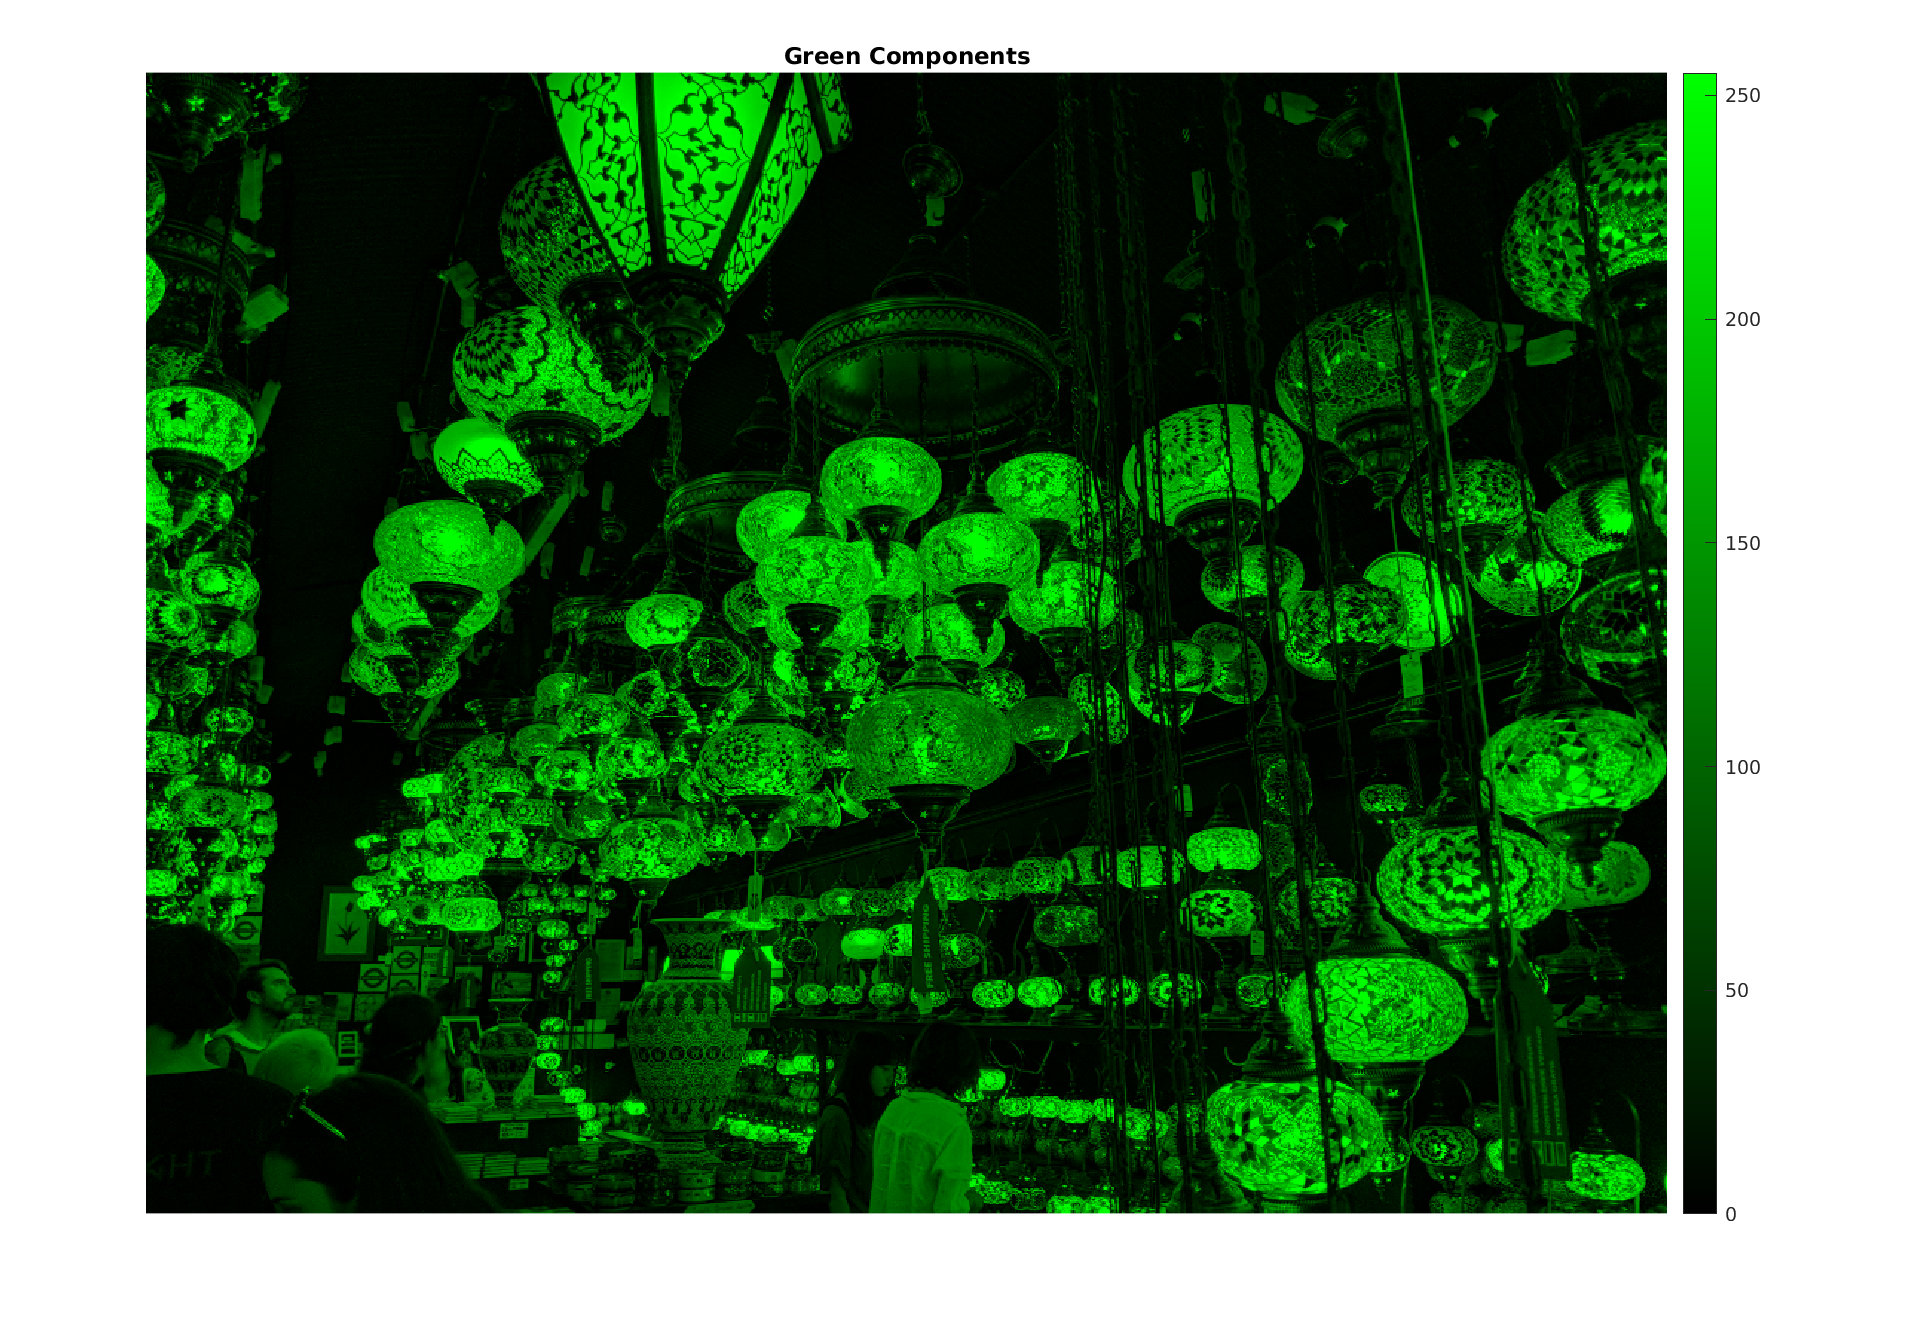
\includegraphics[width=\linewidth]{images/task1/colourfulg.png}
  \caption{Green component of Figure \ref{fig:colorful}.}
  \label{fig:colourfulgreen}
\end{figure}

\begin{figure}[h]
  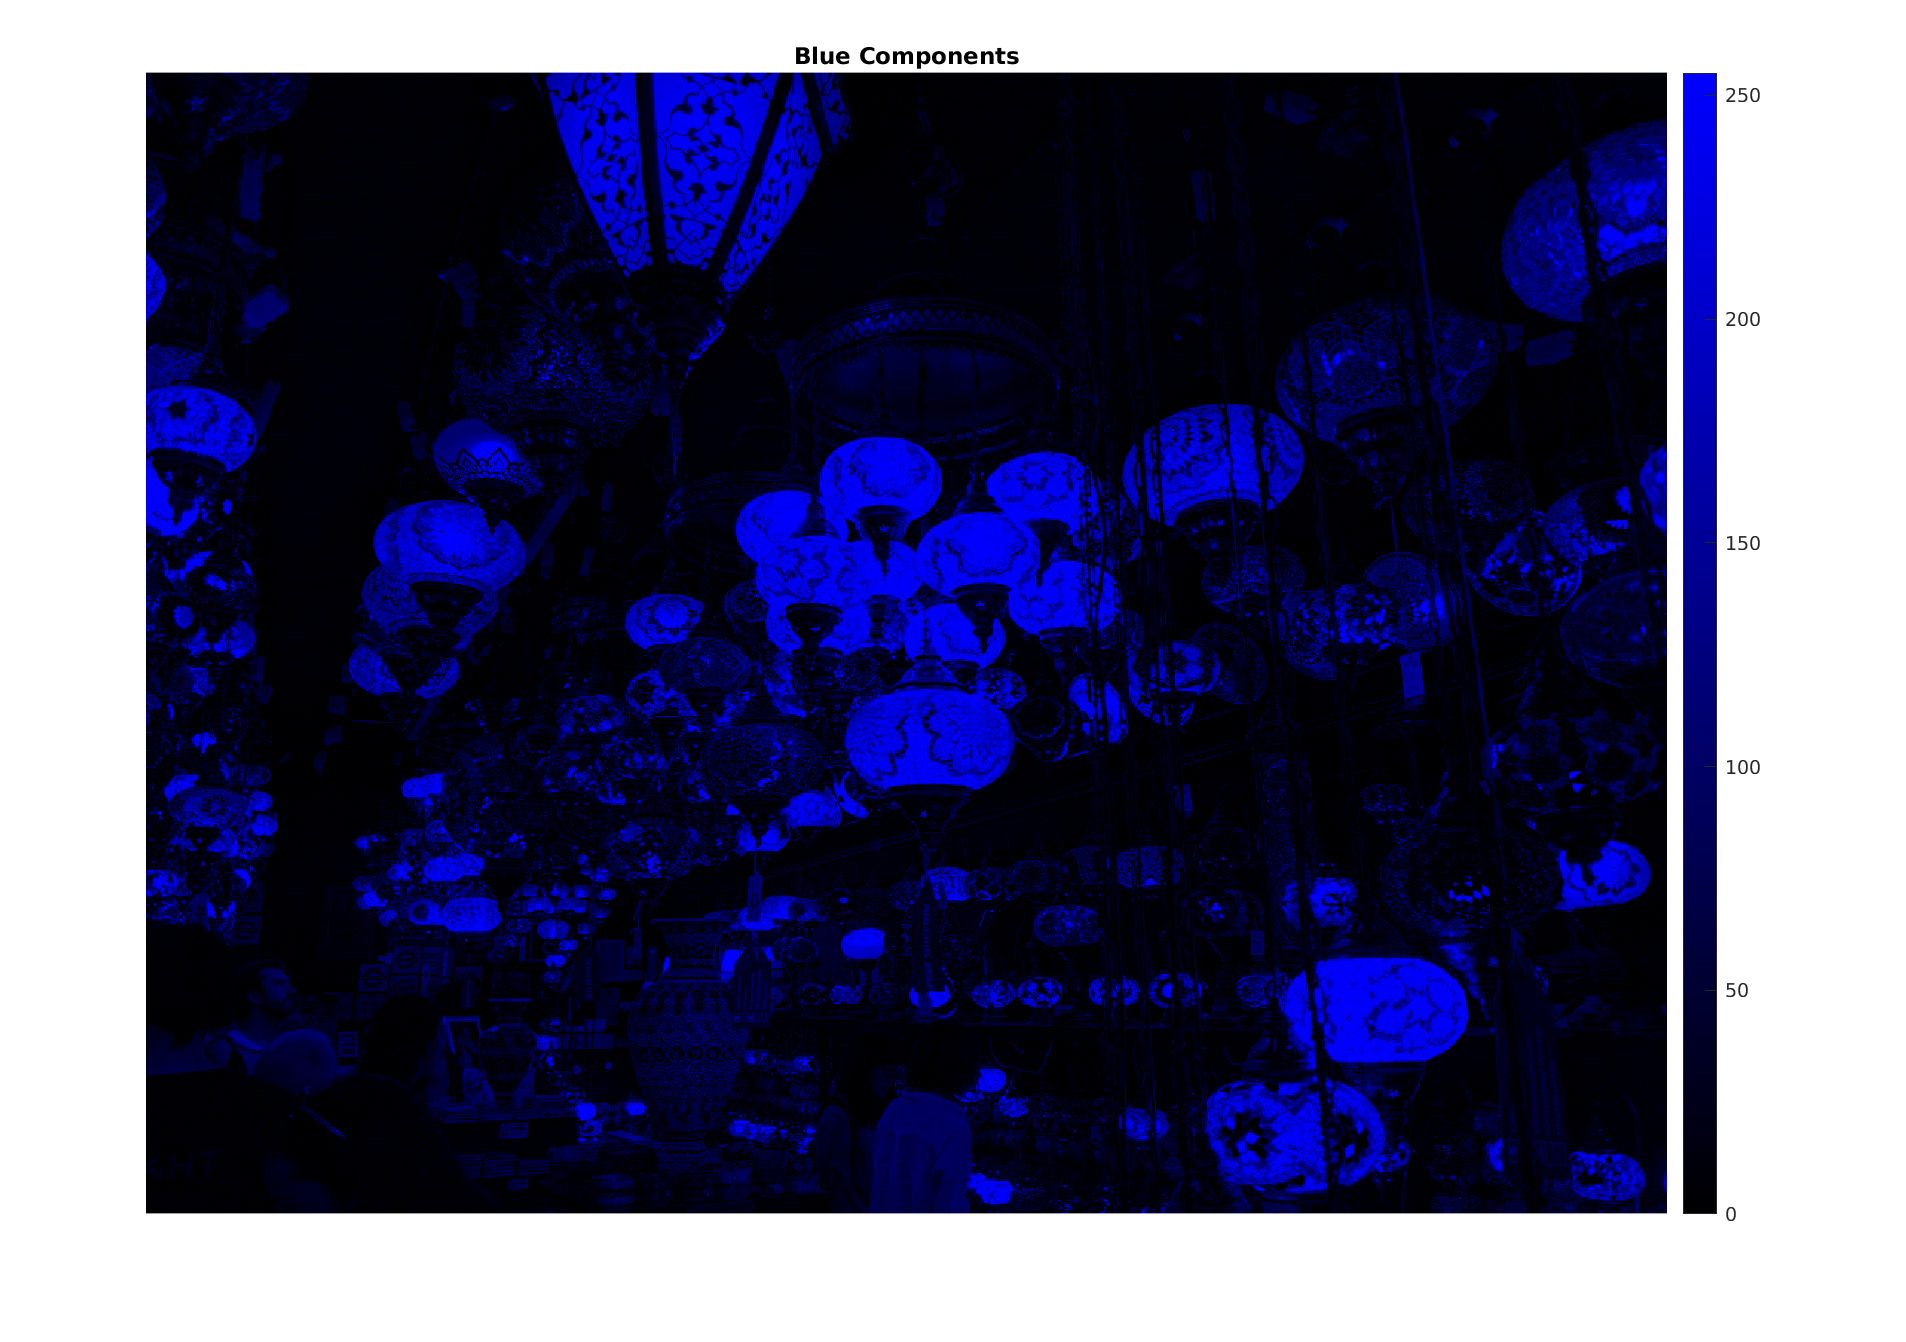
\includegraphics[width=\linewidth]{images/task1/colourfulb.png}
  \caption{Blue component of Figure \ref{fig:colorful}.}
  \label{fig:colourfulblue}
\end{figure}

Figure \ref{fig:simple} was filtered into figures \ref{fig:simplered}, \ref{fig:simplegreen}, and \ref{fig:simpleblue}. Since the image is mostly white, there is very little difference in the three channels.

\begin{figure}[h]
  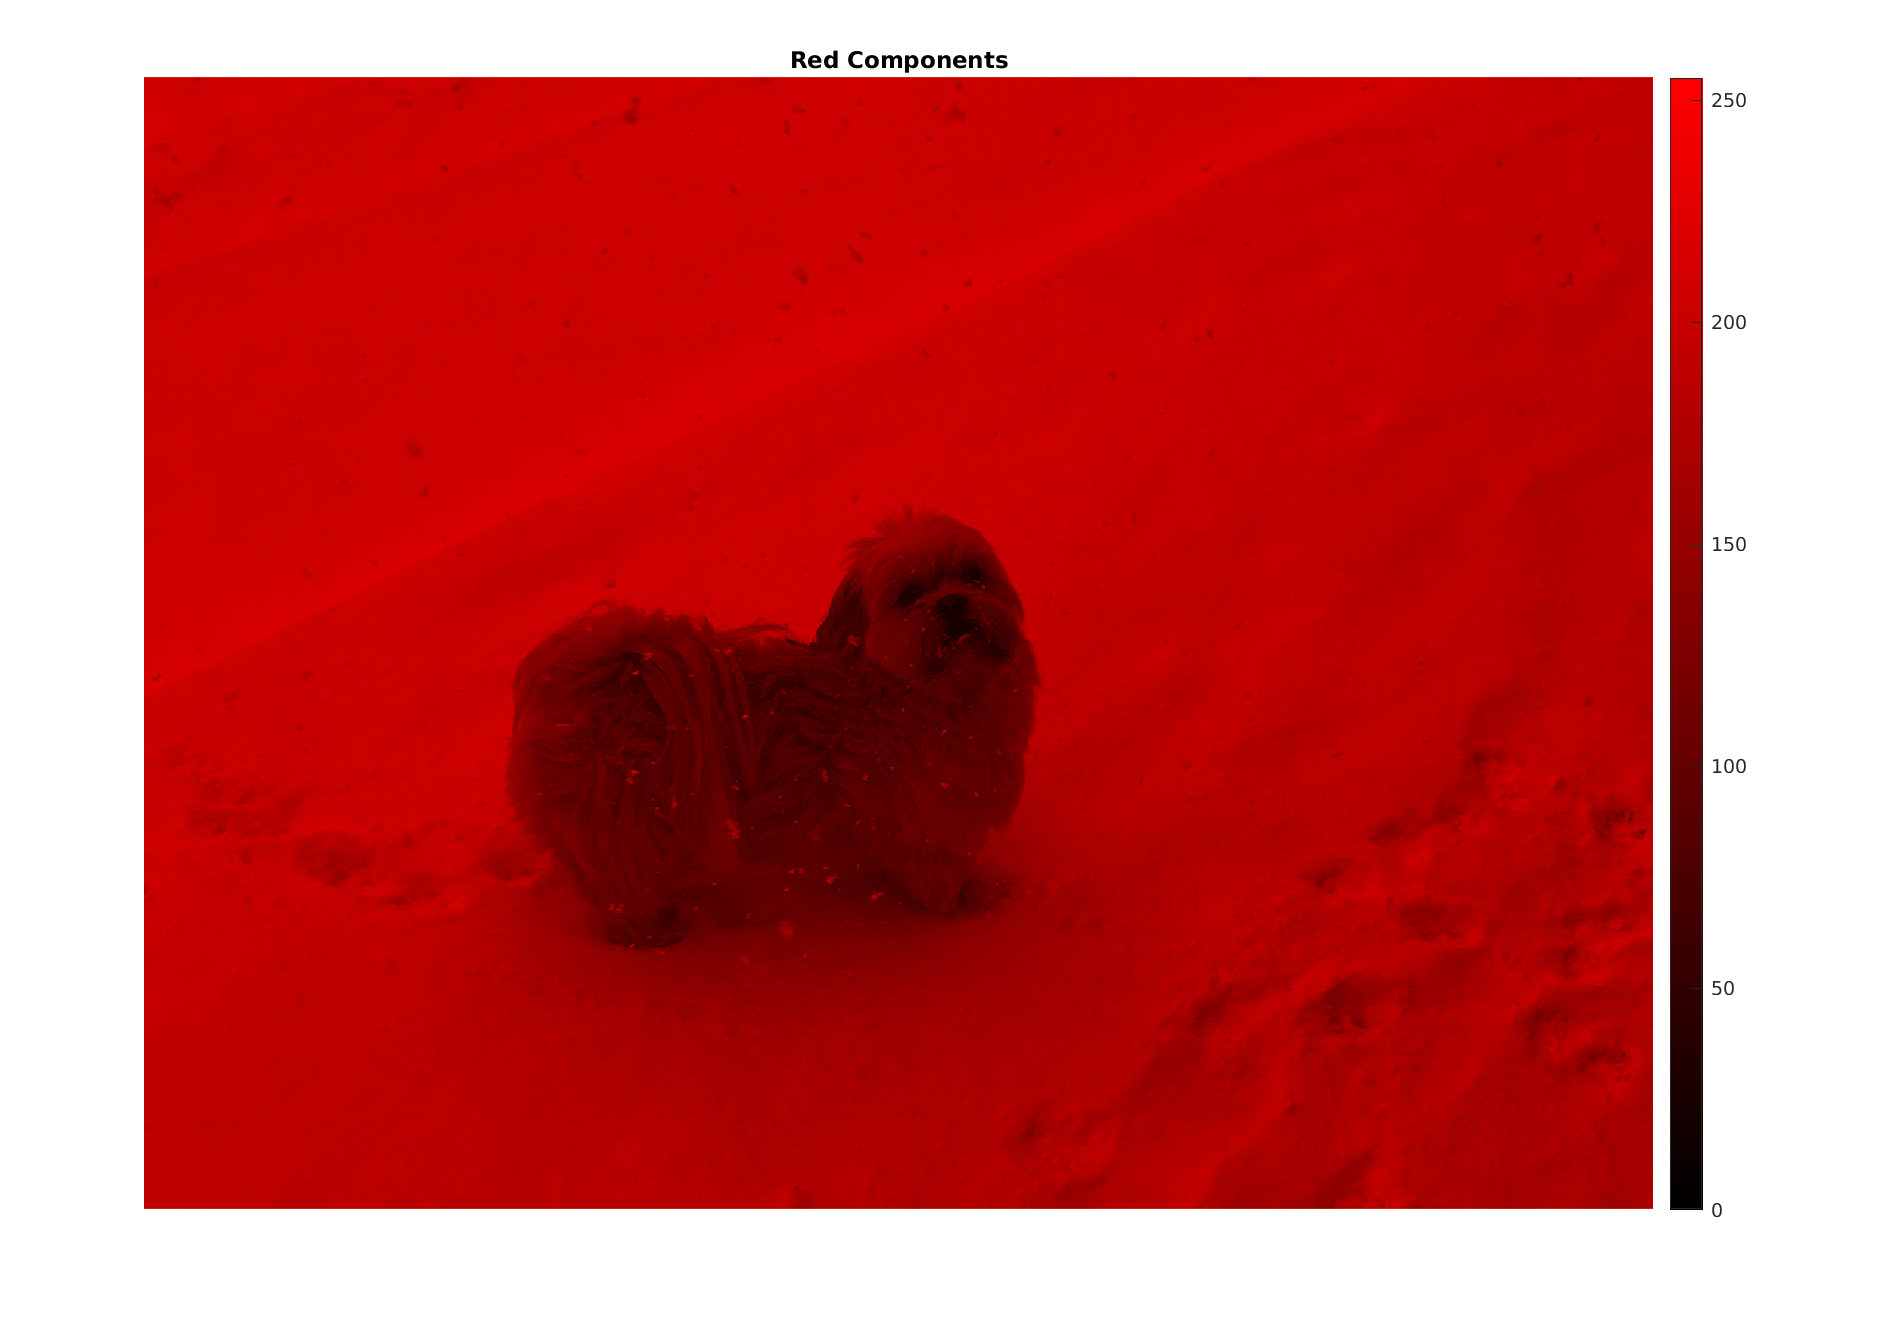
\includegraphics[width=\linewidth]{images/task1/simpler.png}
  \caption{Red component of Figure \ref{fig:simple}.}
  \label{fig:simplered}
\end{figure}

\begin{figure}[h]
  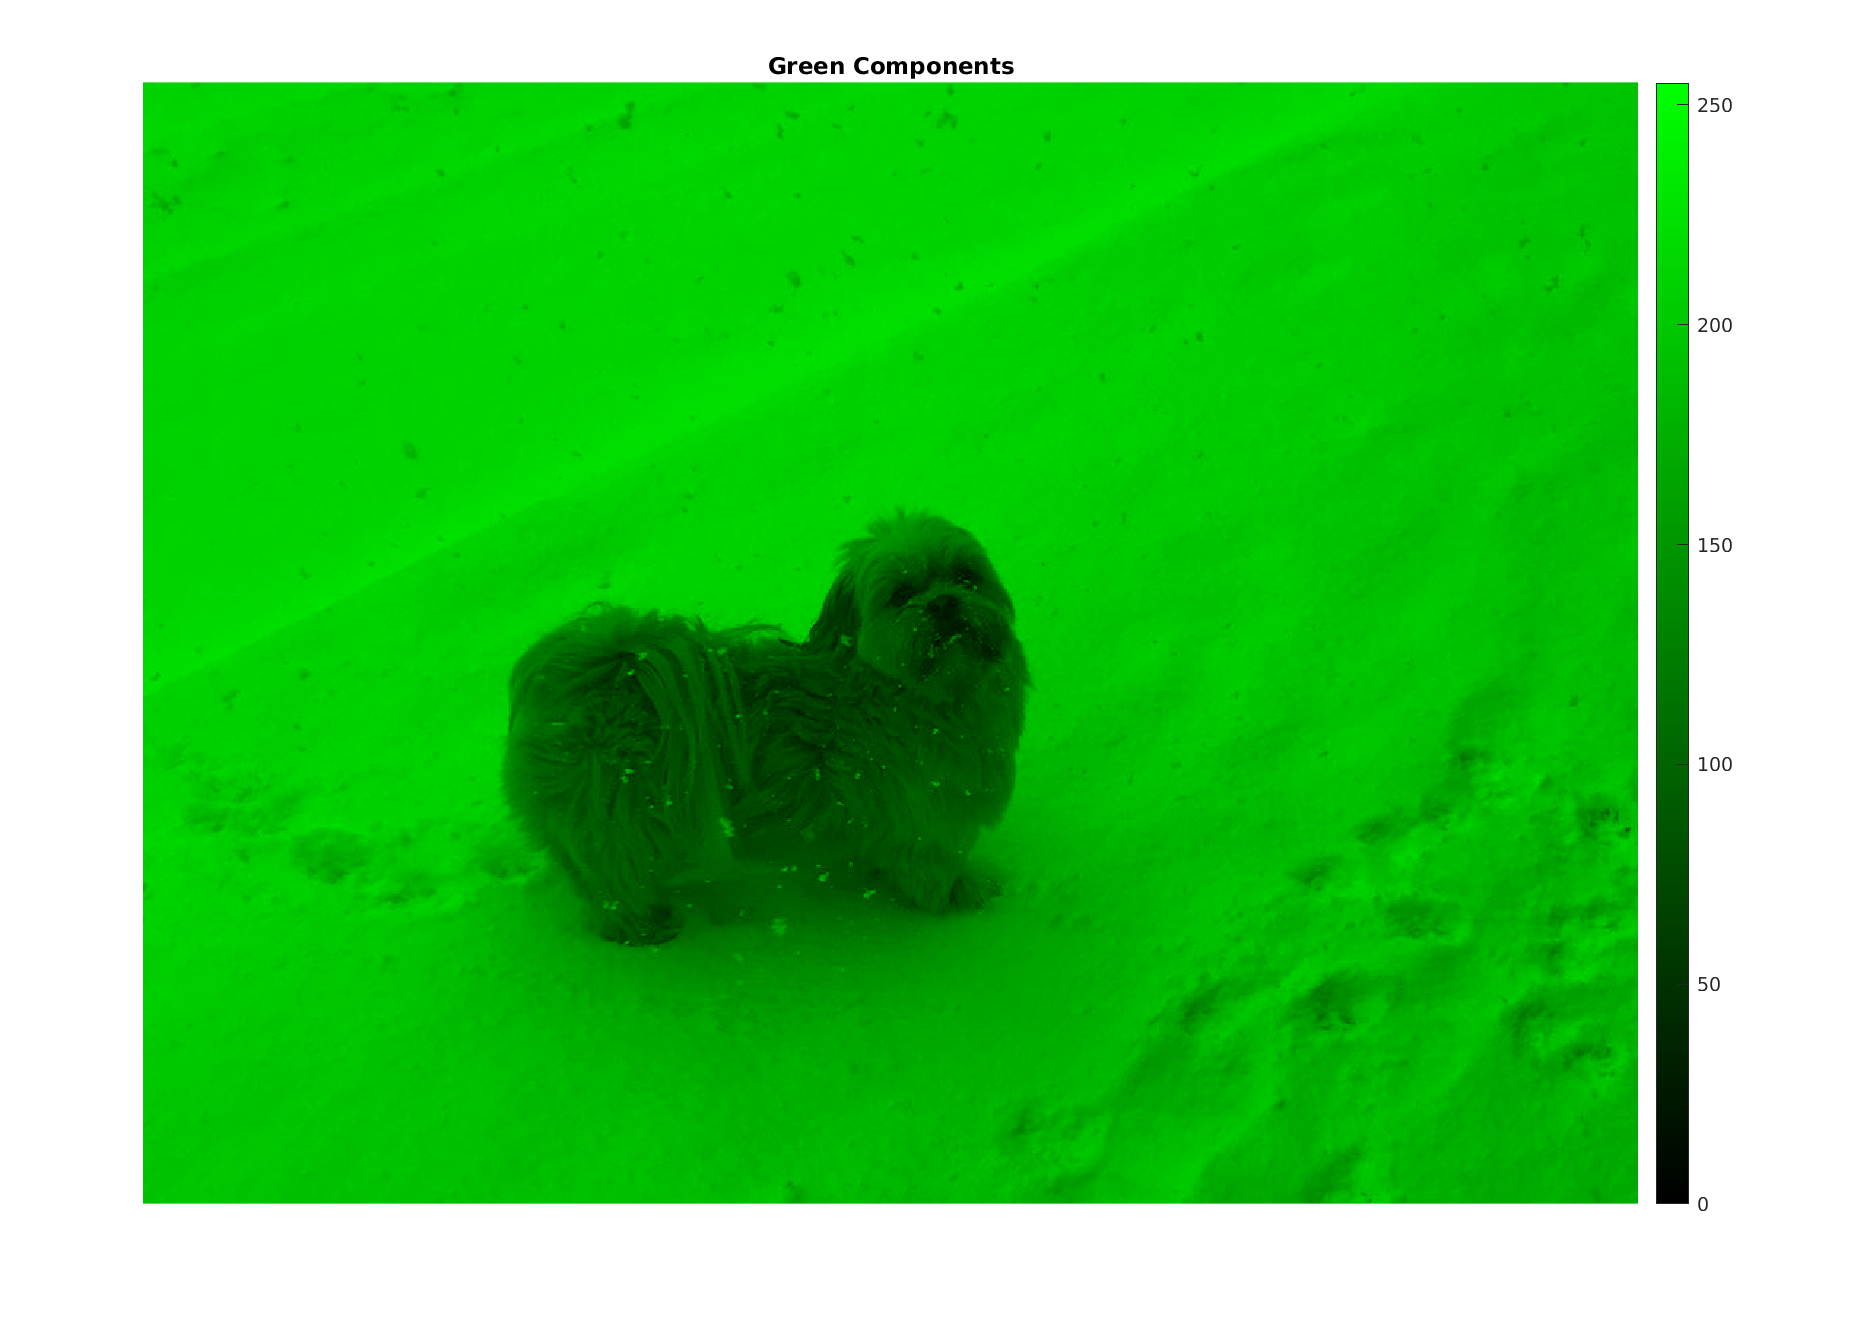
\includegraphics[width=\linewidth]{images/task1/simpleg.png}
  \caption{Green component of Figure \ref{fig:simple}.}
  \label{fig:simplegreen}
\end{figure}

\begin{figure}[h]
  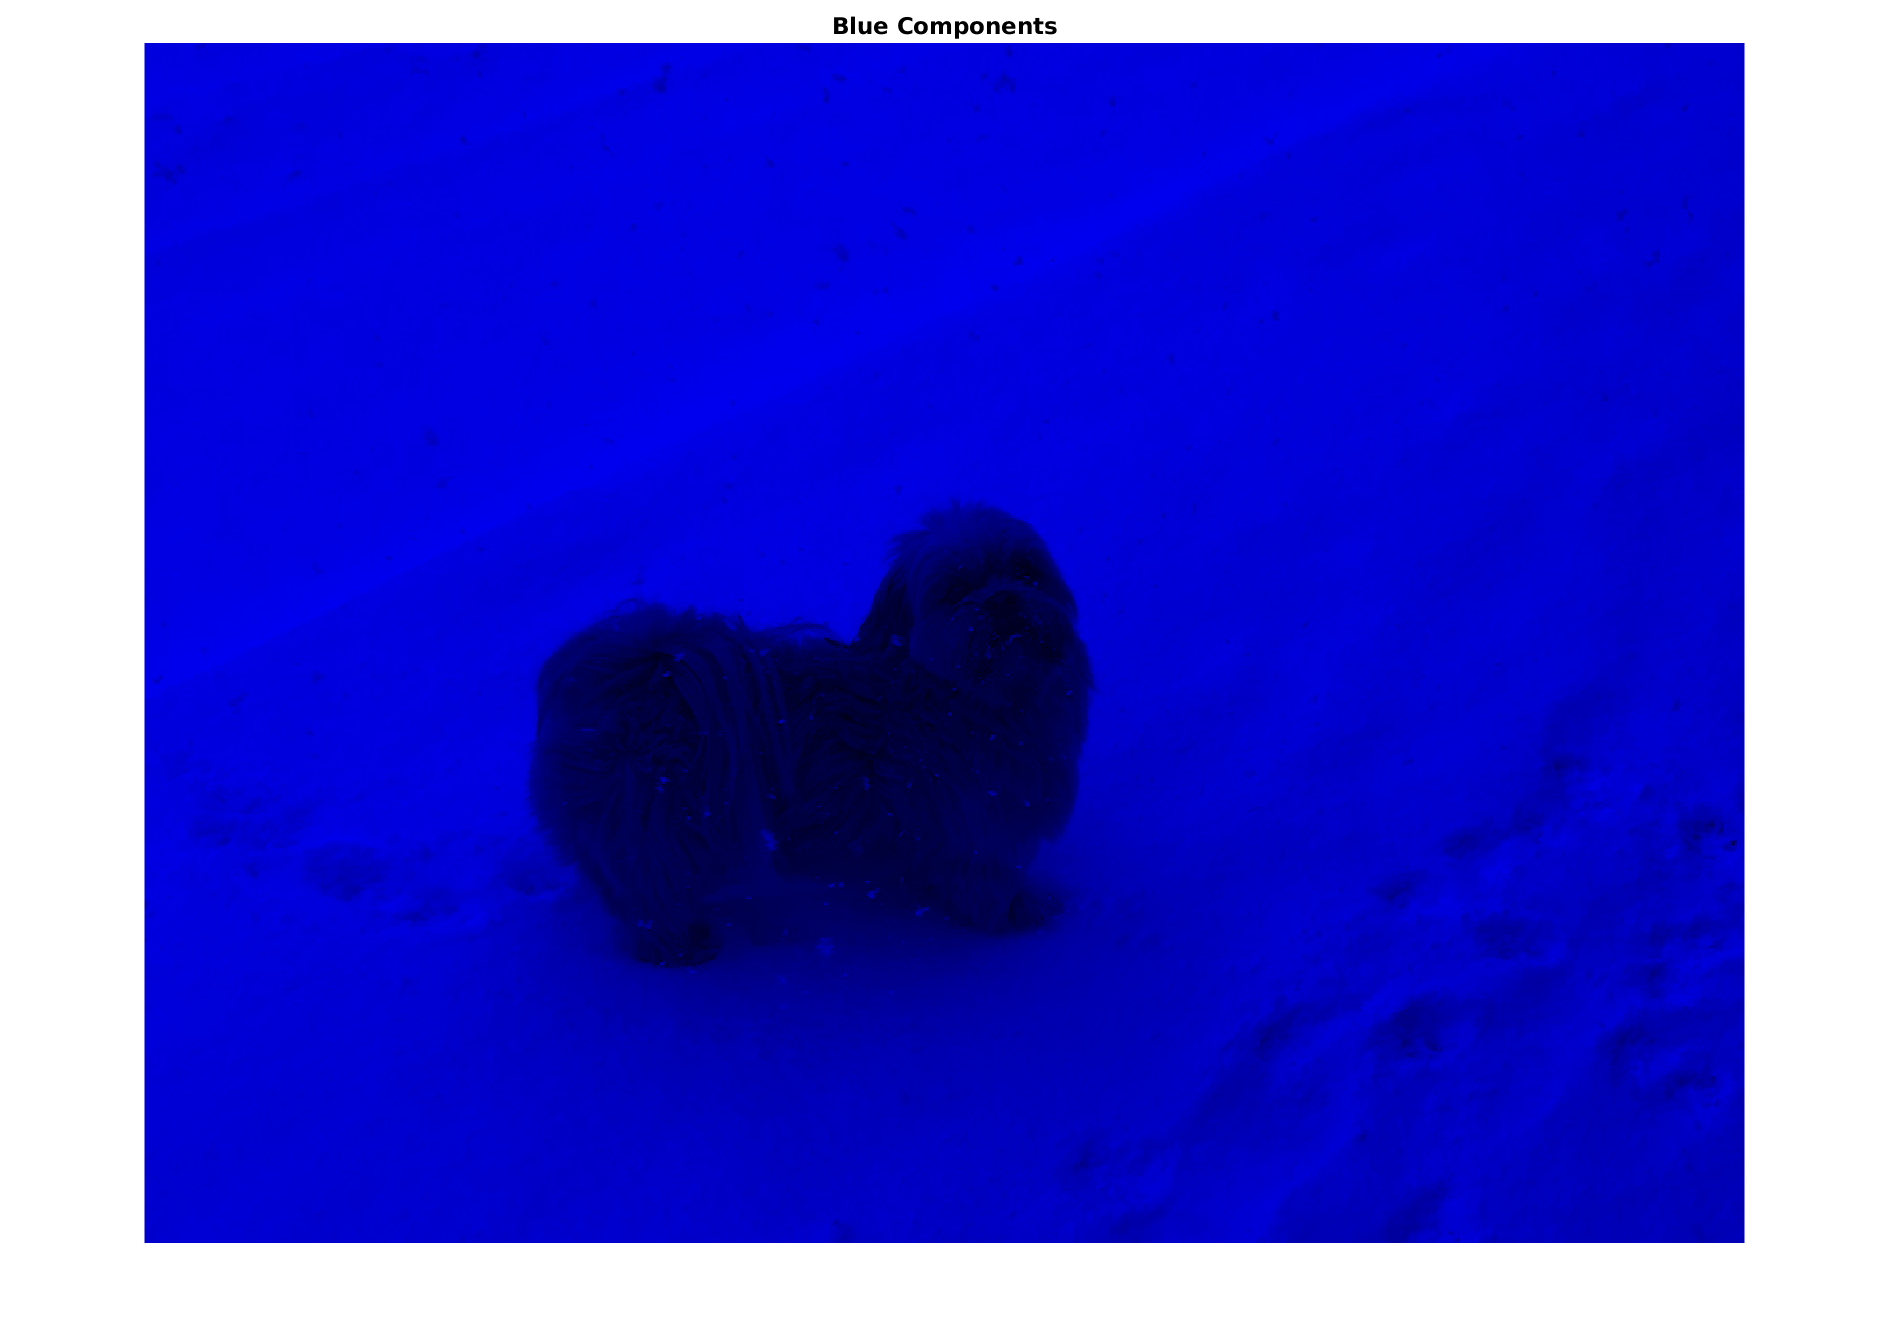
\includegraphics[width=\linewidth]{images/task1/simpleb.png}
  \caption{Blue component of Figure \ref{fig:simple}.}
  \label{fig:simpleblue}
\end{figure}

Figure \ref{fig:drawingblue} was filtered into figures \ref{fig:drawingred}, \ref{fig:drawinggreen}, and \ref{fig:drawingblue}. The rasterized vector image has the most obvious differences compared to the original image. The values of 0 are used for all three channels for the originally transparent background, and so the black text is lost. In the red image (Figure \ref{fig:drawingred}), the blue pentagon is lost. The varying shades of pink in the image appear to be the result of increasing the brightness (the 8-bit value) of the red and blue channels, especially the red.  The square with the colour gradient applied appears a solid colour in the red and blue channels, showing that the green and blue channels are used to produce the white corners.

\begin{figure}[h]
  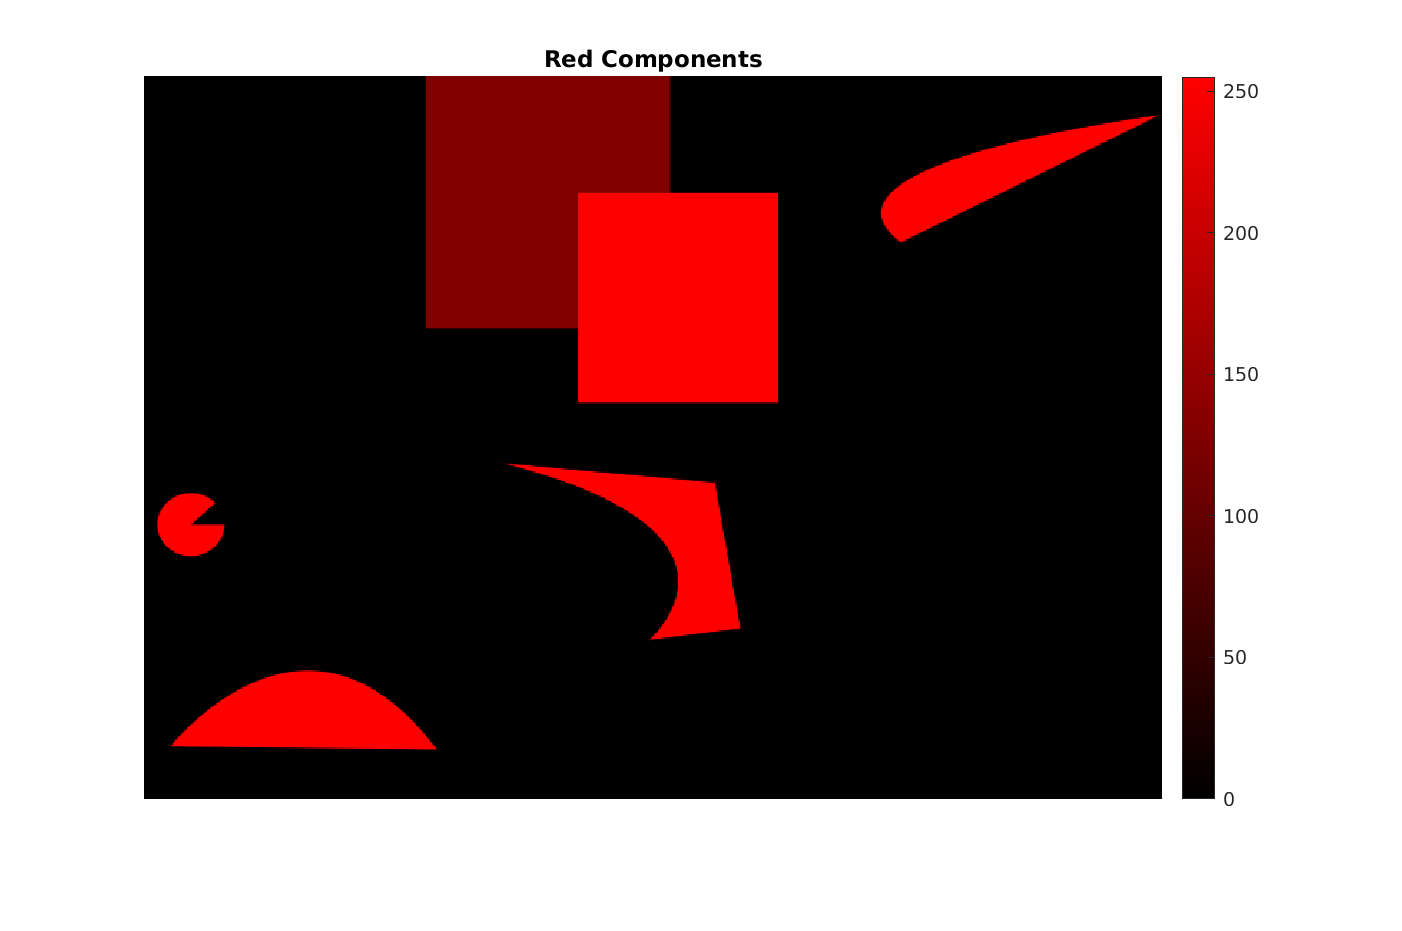
\includegraphics[width=\linewidth]{images/task1/drawingr.png}
  \caption{Red component of Figure \ref{fig:drawing}.}
  \label{fig:drawingred}
\end{figure}

\begin{figure}[h]
  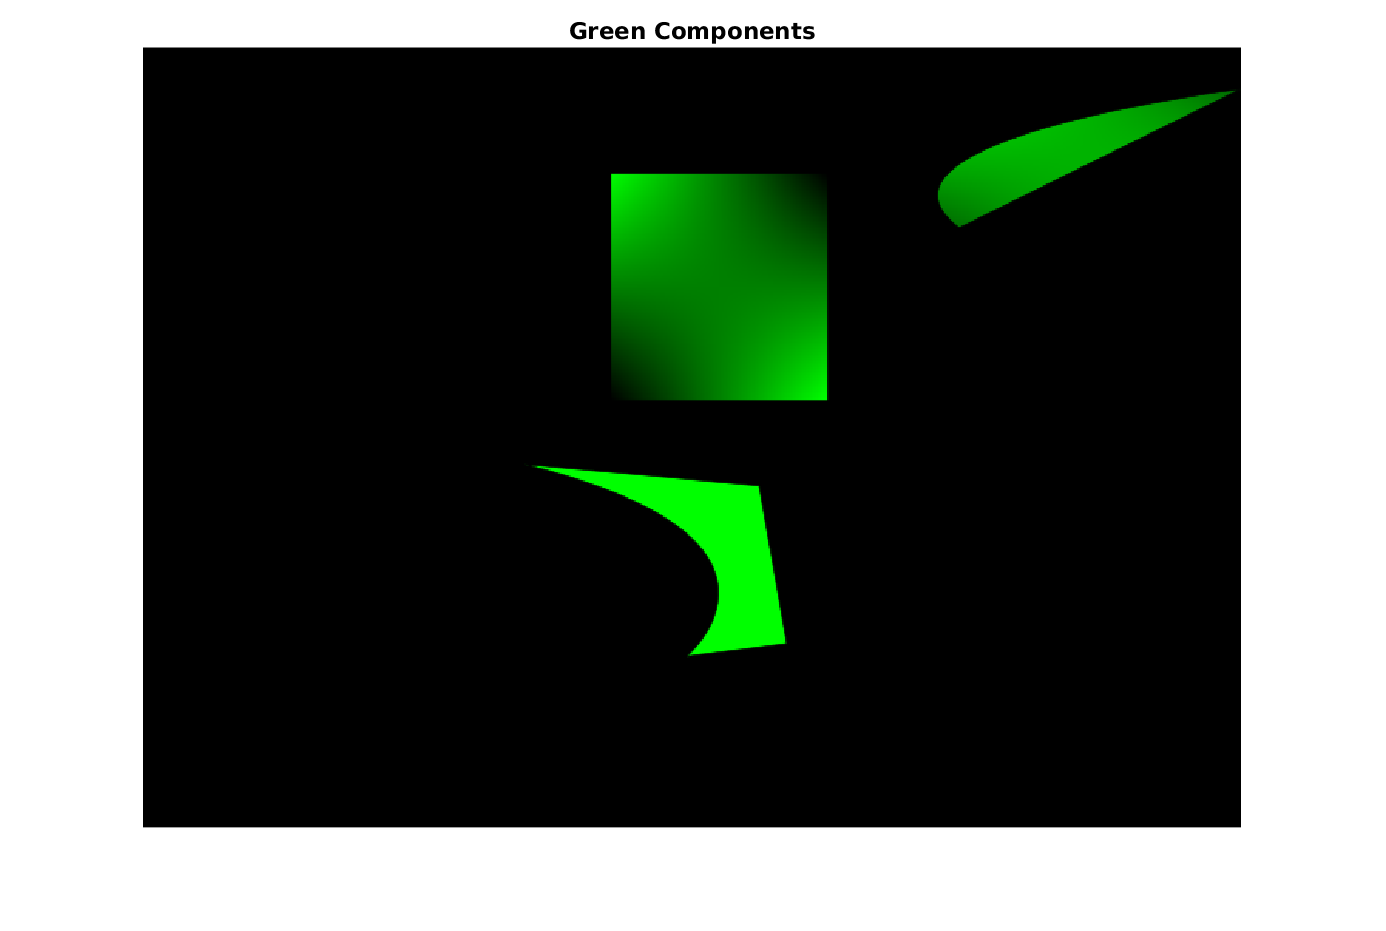
\includegraphics[width=\linewidth]{images/task1/drawingg.png}
  \caption{Green component of Figure \ref{fig:drawing}.}
  \label{fig:drawinggreen}
\end{figure}

\begin{figure}[h]
  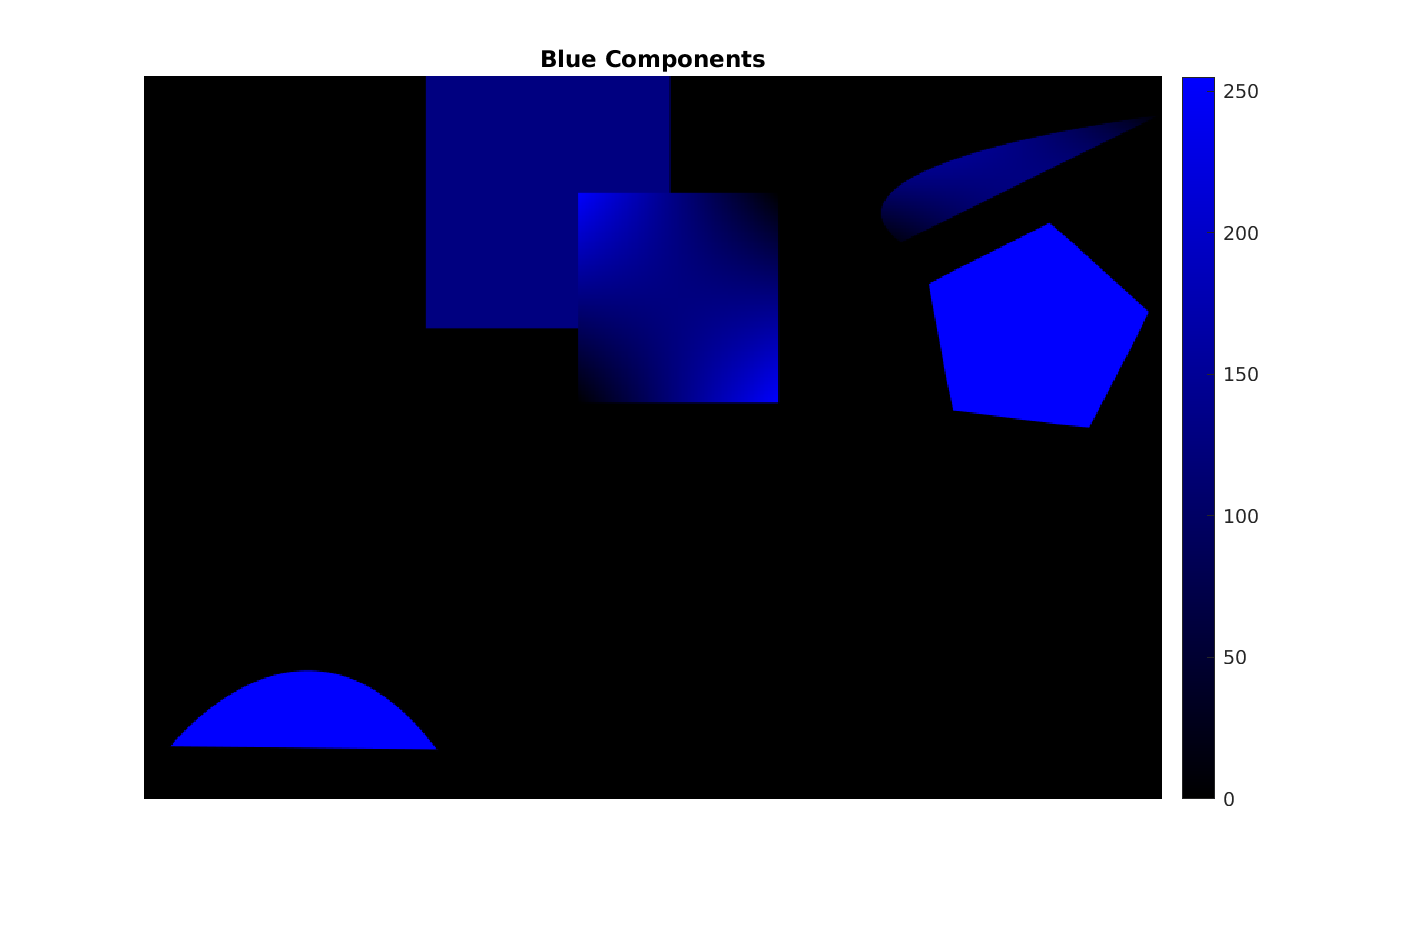
\includegraphics[width=\linewidth]{images/task1/drawingb.png}
  \caption{Blue component of Figure \ref{fig:drawing}.}
  \label{fig:drawingblue}
\end{figure}

\section{YCbCr}

For this task, I used both inbuilt \emph{rgb2ycbcr} and \emph{ycbcr2rgb} methods, and then implemented my own respective versions \emph{rgbToYCbCr} and \emph{YCbCrToRGB} in order to better understand the transformation. 
The equations for the translation between the two colour spaces are shown in equations \ref{eq:RGBToYCbCr} and \ref{eq:YCbCrtoRGB} \cite{jpegformatspec}. These equations are specifically for the translation between 8-bit RGB and 256 level YCbCr. In order to ensure that the resulting YCbCr values occupy the full 256 levels available, the values of RGB would have to be normalised if not already 8-bit. 

\begin{flalign} \label{eq:RGBToYCbCr}
	\begin{aligned}
	&y = 0.299r + 0.587g + 0.114b &\\
	&Cb= -0.1687r - 0.3313g + 0.5b + 128 &\\
	&Cr= 0.5r - 0.4187g - 0.0813b + 128 &
	\end{aligned}
\end{flalign}

\begin{flalign} 
	\begin{aligned} \label{eq:YCbCrtoRGB}
	&r = y + 1.402(Cr - 128) &\\
	&g = y - 0.34414(Cb - 128) - 0.71414(Cr - 128) &\\
	&b = y + 1.772(Cb - 128) &
	\end{aligned}
\end{flalign}

Often when transmitted, YCbCr encoders will instead use the range of 16 to 235 for analogue television signals. This is used to combat Gibbs phenomenon \citep{helmberg_1994}, which is introduced to the signal after filtering. The effect of Gibbs phenomemon is shown in figure \ref{fig:gibbs}. The high frequency components visible at sharp transition points produce unwanted artifacts in the signal. This is likely also the reason for the metallic ringing sound from the previous practical when a band of frequencies were zeroed from after performing an FFT, and why more effective filters use a gradual reduction in magnitude. The footroom and headrooom supplied by these unused bits are sometimes also used to store metadata on more reliable signals. The Matlab documentation for \emph{rgb2ycbcr} states that it uses the analogue translation for YCbCr which includes footroom and headroom \cite{matlabrgb2ycbcr}.

\begin{figure}[h]
  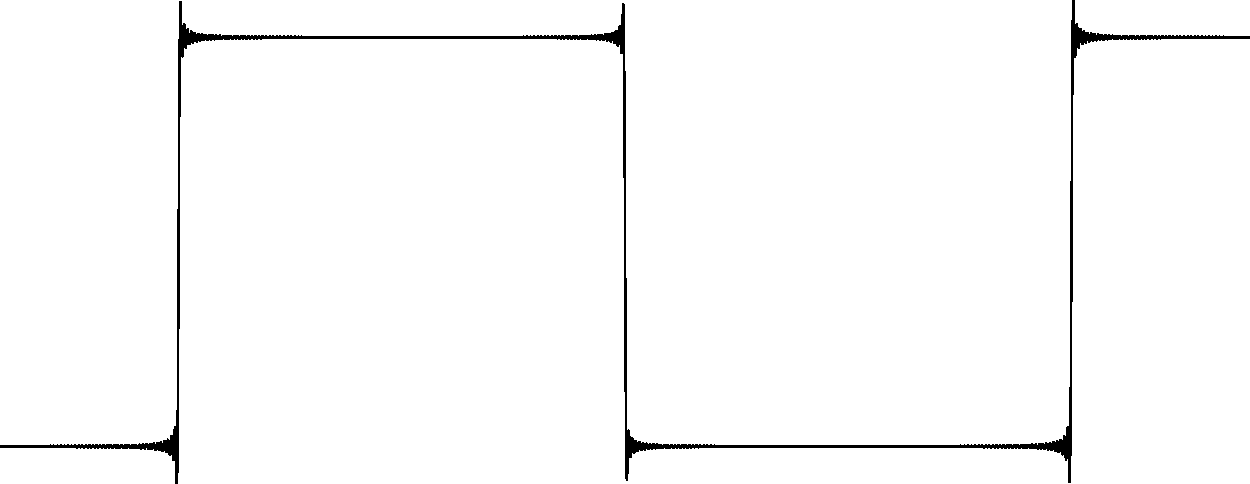
\includegraphics[width=\linewidth]{images/gibbs.pdf}
  \caption{Gibbs Phenomenon when Approximating a Square Signal\cite{gibbs}.}
  \label{fig:gibbs}
\end{figure}

The custom implementations produced Figures \ref{fig:customYCbCrColourful}, \ref{fig:customYCbCrDrawing}, and \ref{fig:customYCbCrSimple}. The top left image for each figure is the result of \emph{imshow} on YCbCr values, where the YCbCr values are being incorrectly interpreted as RGB. In order to render the YCbCr components as RGB using \emph{imshow} correctly, all other layers except the one being considered had to be 'zeroed'. The zero value for the Y component (luminance) is actually 0, as this corresponds to no signal. However, for Cb and Cr (Chromatic blue and red, respectively), the value of 128 was used corresponds to no signal, as this represents black. 

\begin{figure}[h]
  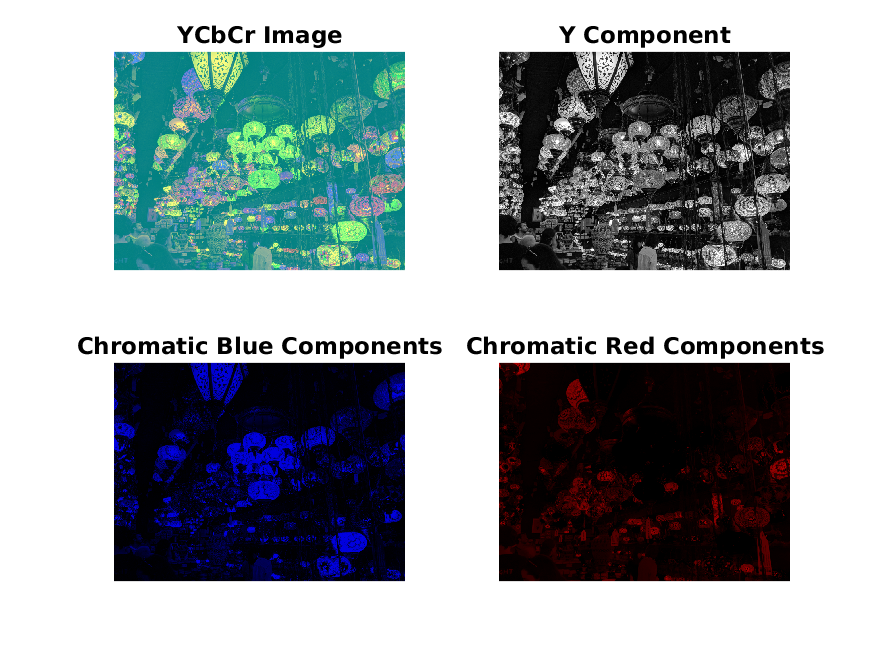
\includegraphics[width=\linewidth]{images/task2/colourfulcustom.png}
  \caption{Custom YCbCr translation of Figure \ref{fig:colorful}.}
  \label{fig:customYCbCrColourful}
\end{figure}

\begin{figure}[h]
  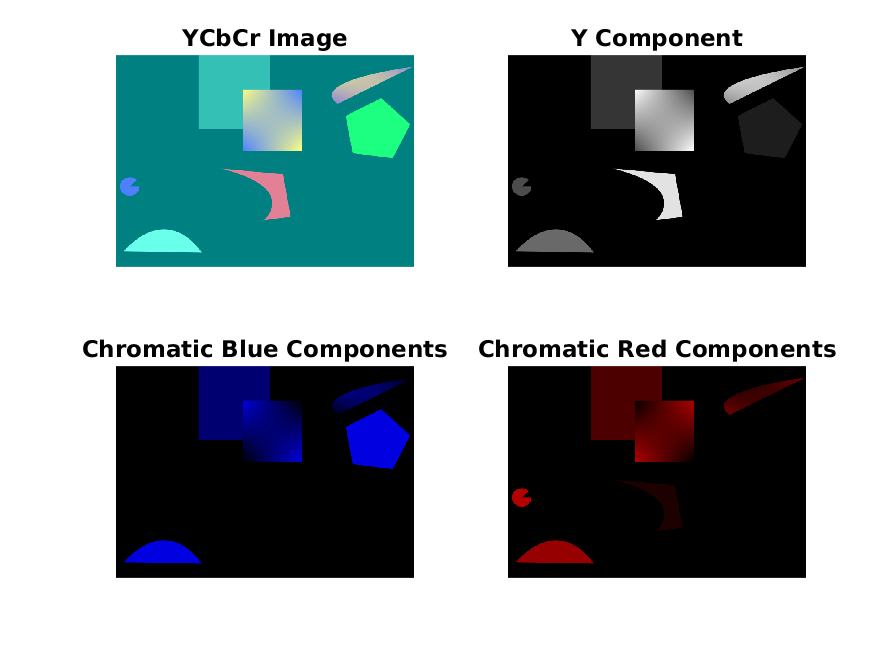
\includegraphics[width=\linewidth]{images/task2/drawingcustom.png}
  \caption{Custom YCbCr translation of Figure \ref{fig:drawing}.}
  \label{fig:customYCbCrDrawing}
\end{figure}

\begin{figure}[h]
  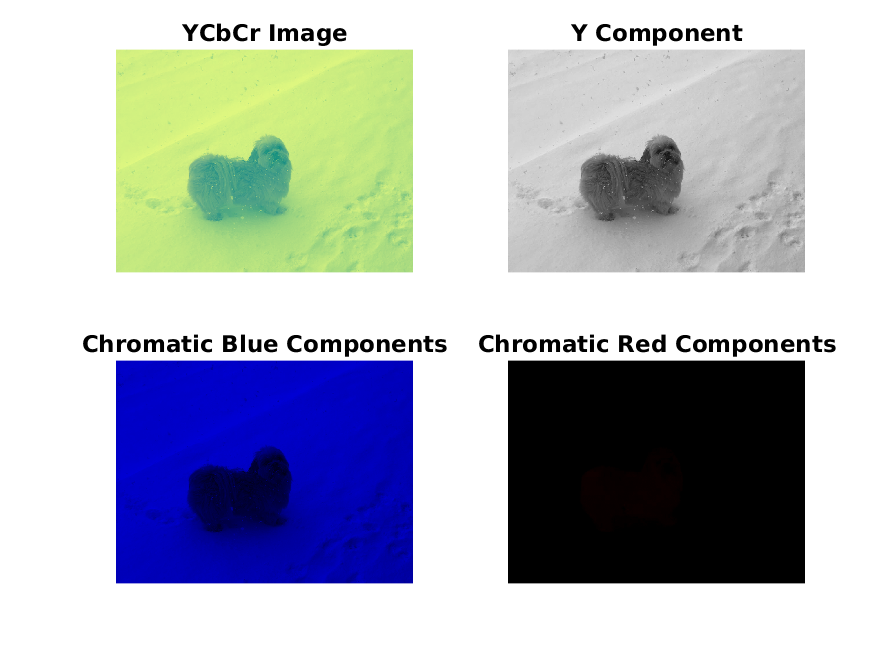
\includegraphics[width=\linewidth]{images/task2/simplecustom.png}
  \caption{Custom YCbCr translation of Figure \ref{fig:simple}.}
  \label{fig:customYCbCrSimple}
\end{figure}

The inbuilt functions produced figures \ref{fig:colourfuly}-\ref{fig:simplecr}. Comparing the results, the values of chromaticity from the custom implementation appear lower than the inbuilt functions. This is especially evident when comparing the Cb components produced from figure \ref{fig:simple} (Figures \ref{fig:customYCbCrSimple} and \ref{fig:simplecb}). Since the white snow is the same in greyscale as it is coloured, no chromaticities are needed. However, in the custom implementation, Cb appears to be greater than 128 throughout.

For the components of figure \ref{fig:colorful}, the lighter blue lanters in the centre appear to be composed of low Cr and high Cb values (given the green present in \ref{fig:colourfulcr} and saturated blue in \ref{fig:colourfulcb}). 

\begin{figure}[h]
  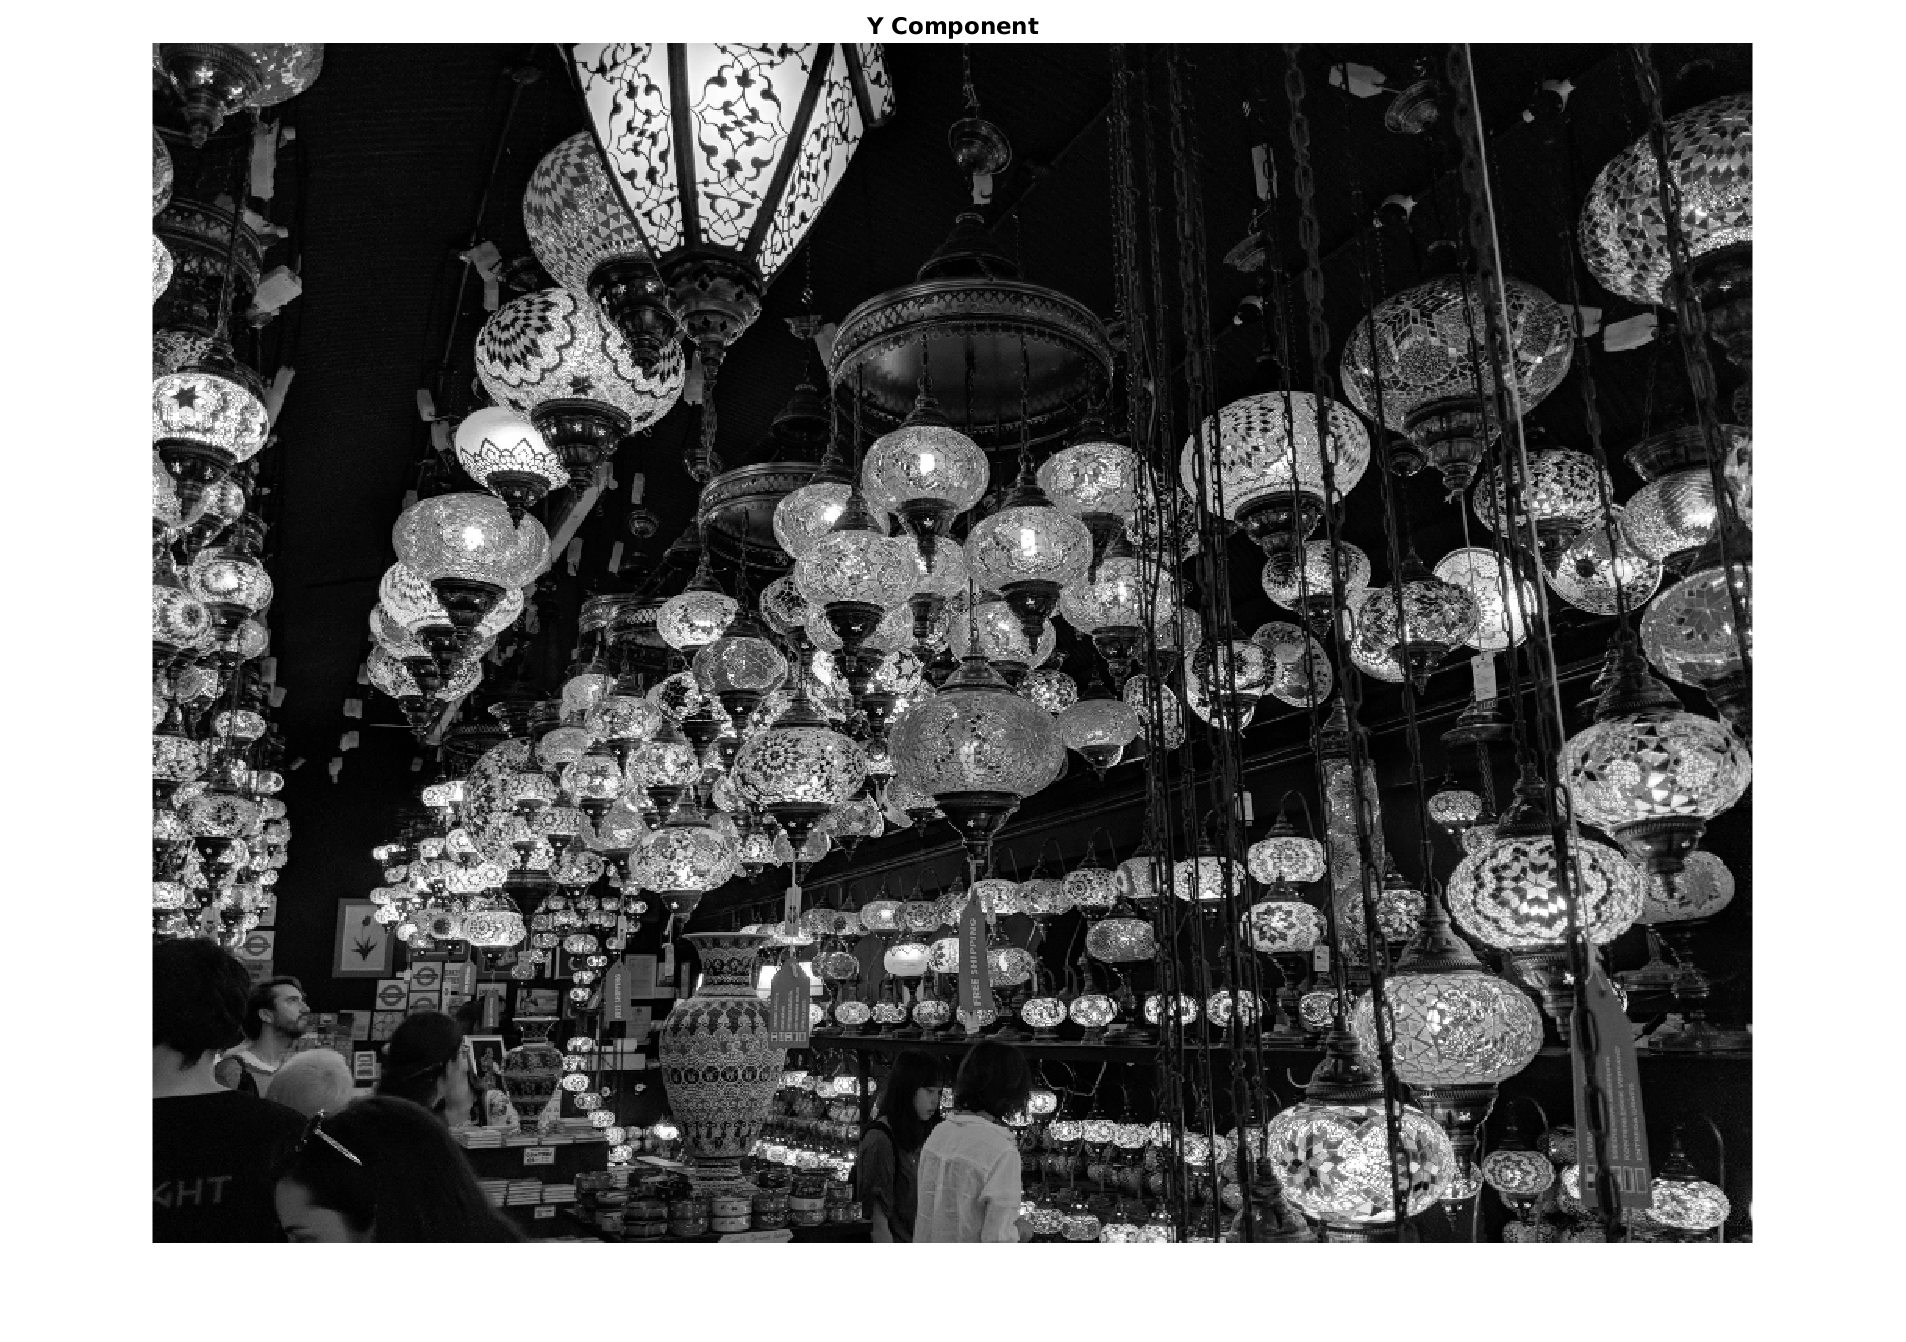
\includegraphics[width=\linewidth]{images/task2/colourfuly.png}
  \caption{Luminance component of Figure \ref{fig:colorful}.}
  \label{fig:colourfuly}
\end{figure}

\begin{figure}[h]
  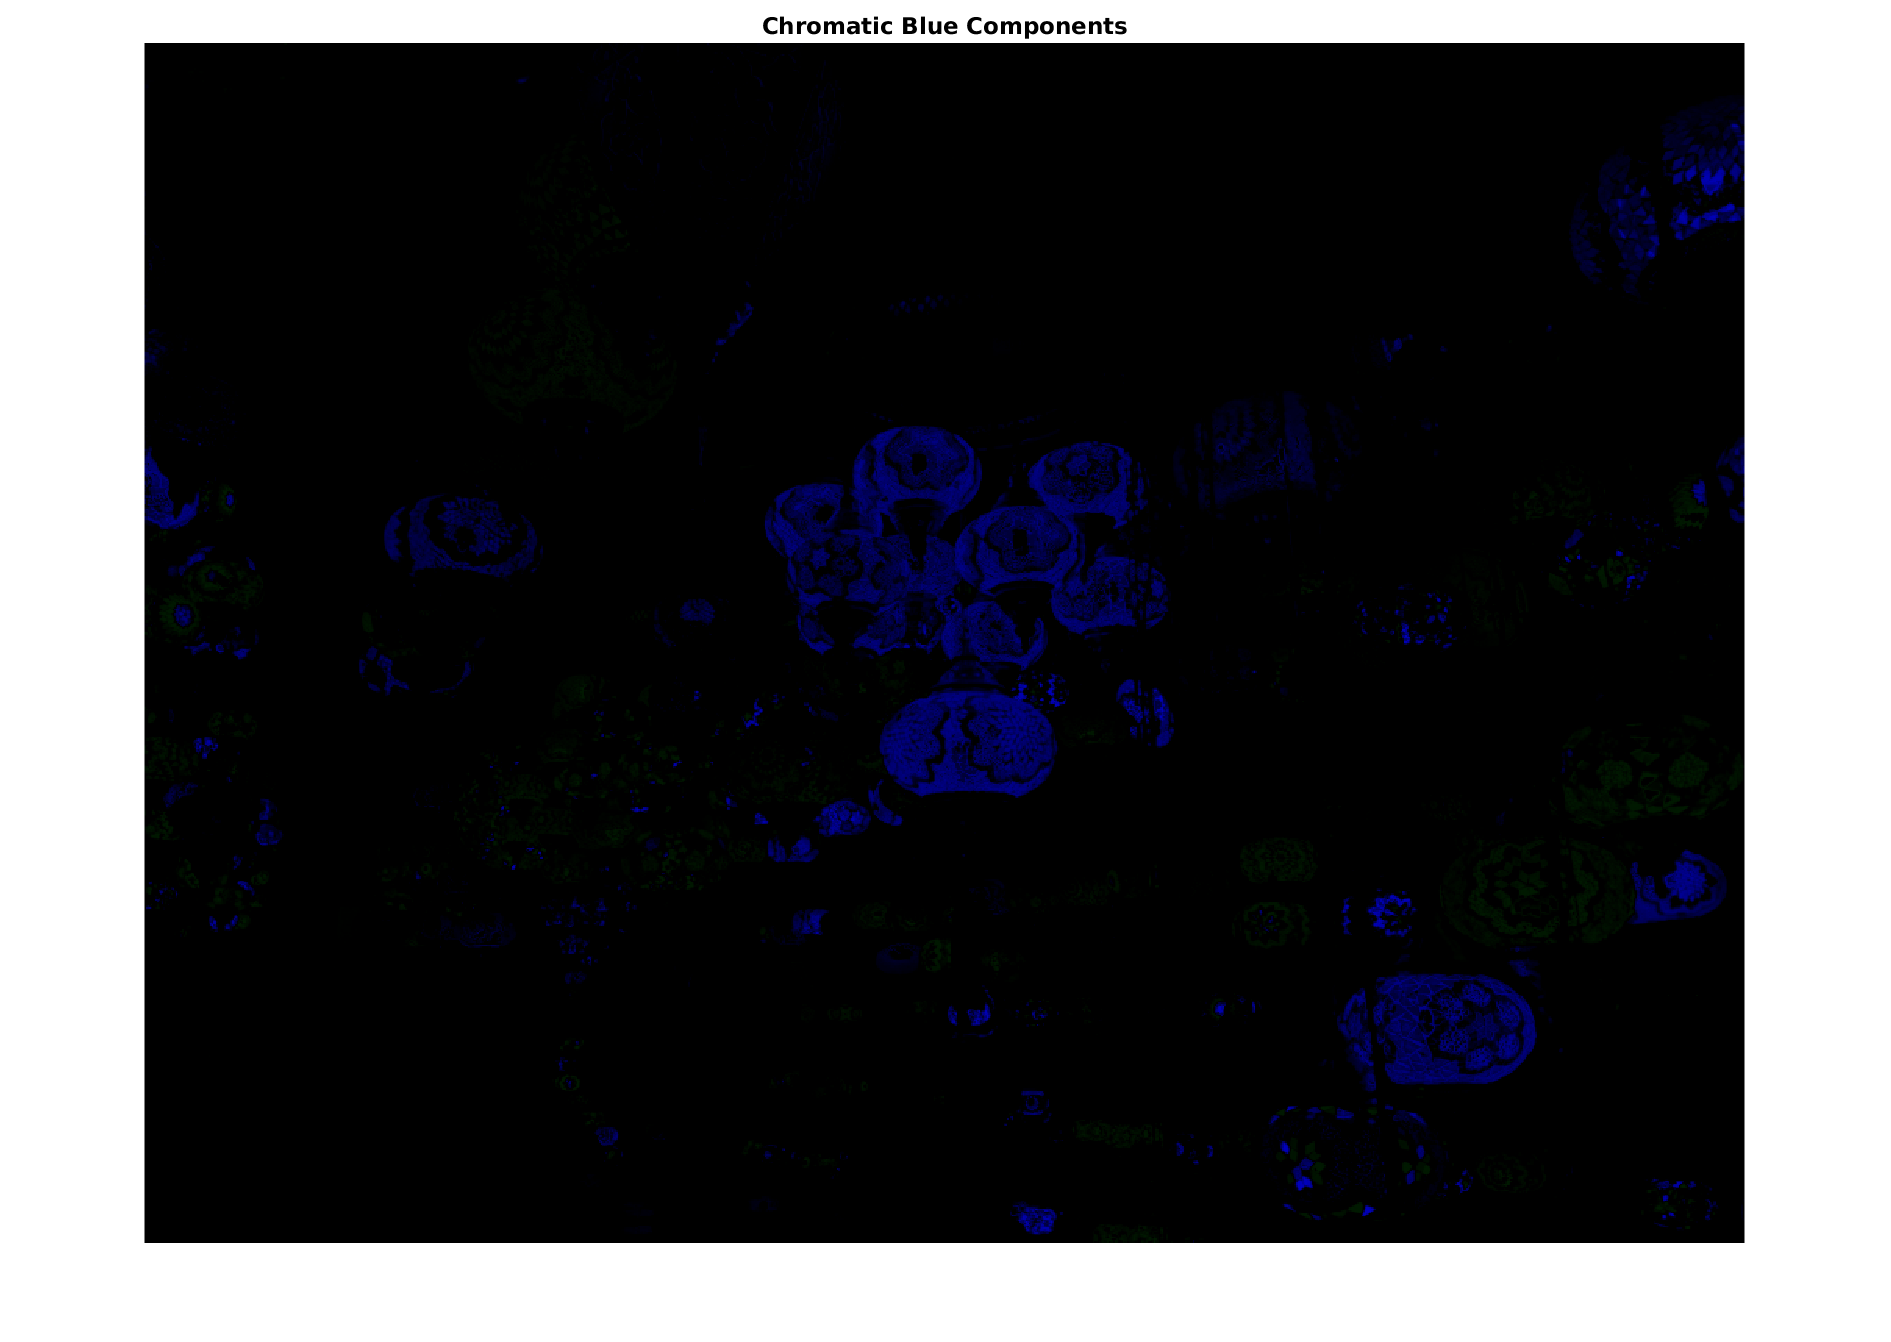
\includegraphics[width=\linewidth]{images/task2/colourfulcb.png}
  \caption{Chromatic Blue component of Figure \ref{fig:colorful}.}
  \label{fig:colourfulcb}
\end{figure}

\begin{figure}[h]
  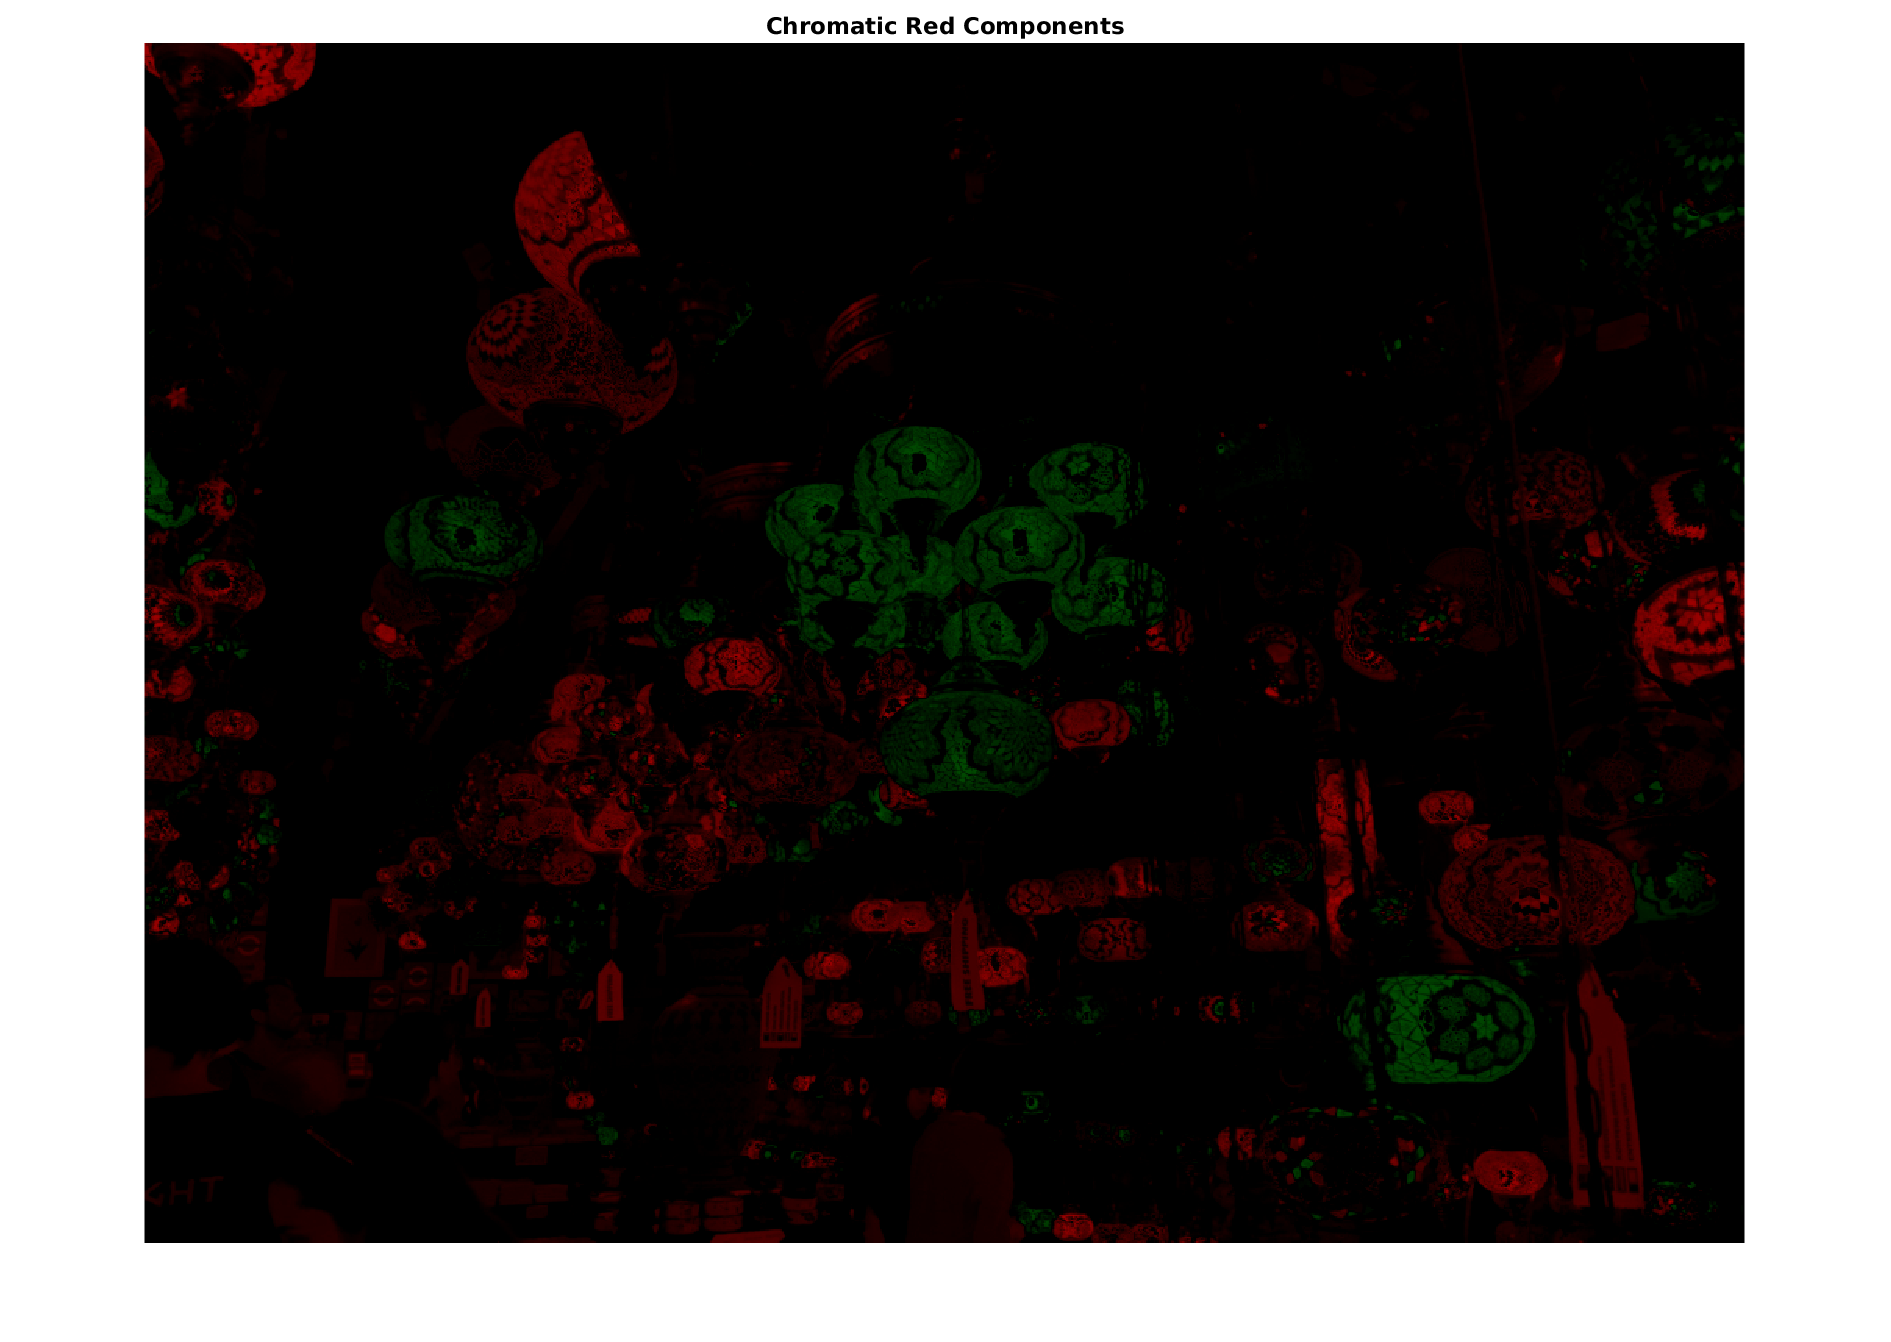
\includegraphics[width=\linewidth]{images/task2/colourfulcr.png}
  \caption{Chromatic Red component of Figure \ref{fig:colorful}.}
  \label{fig:colourfulcr}
\end{figure}

\begin{figure}[h]
  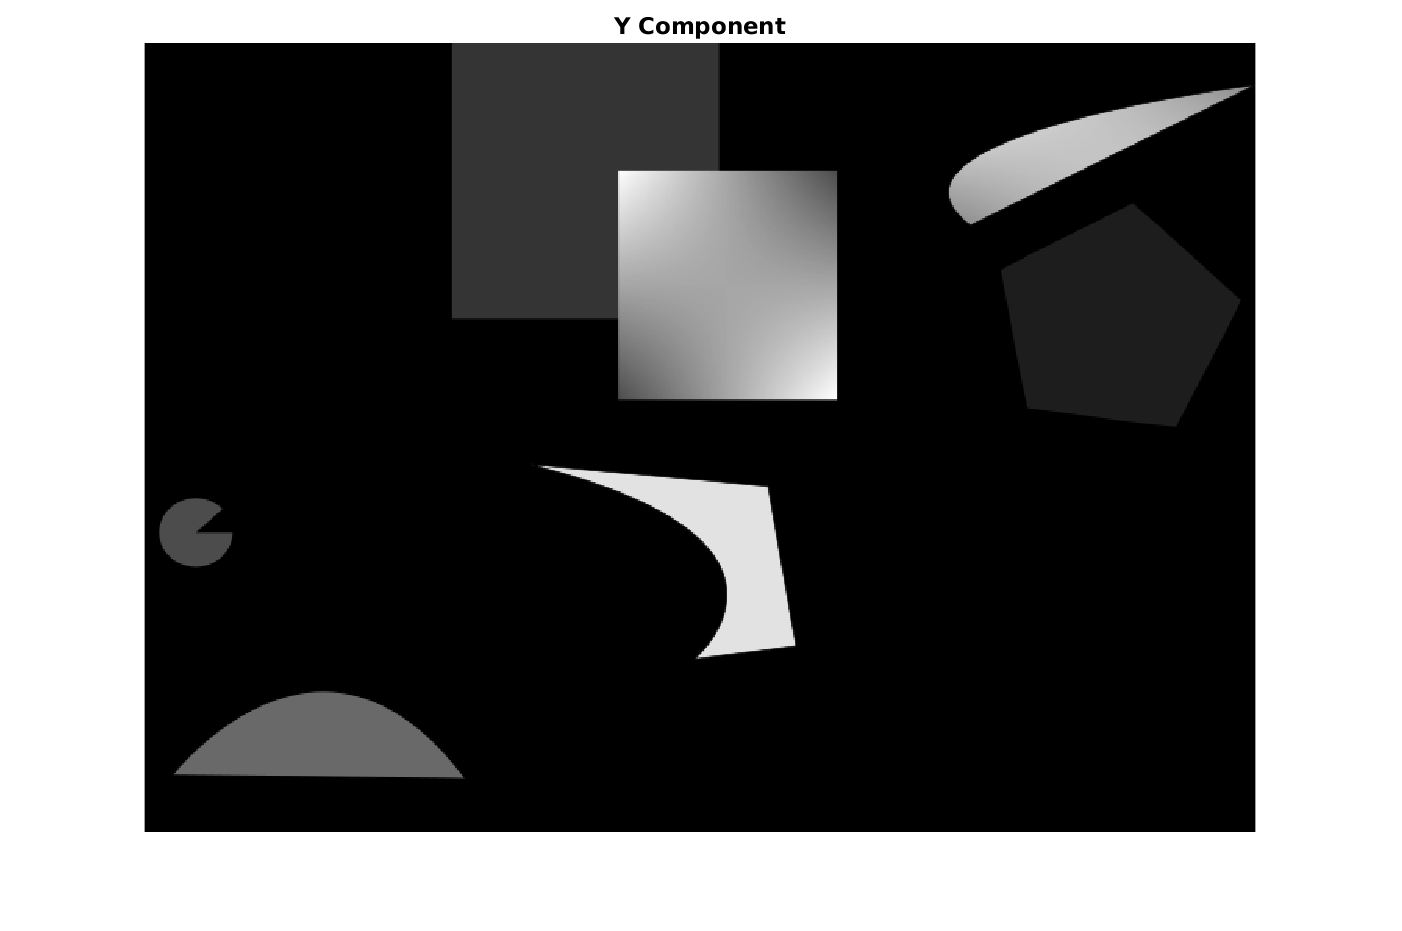
\includegraphics[width=\linewidth]{images/task2/drawingy.png}
  \caption{Luminance component of Figure \ref{fig:drawing}.}
  \label{fig:drawingy}
\end{figure}

\begin{figure}[h]
  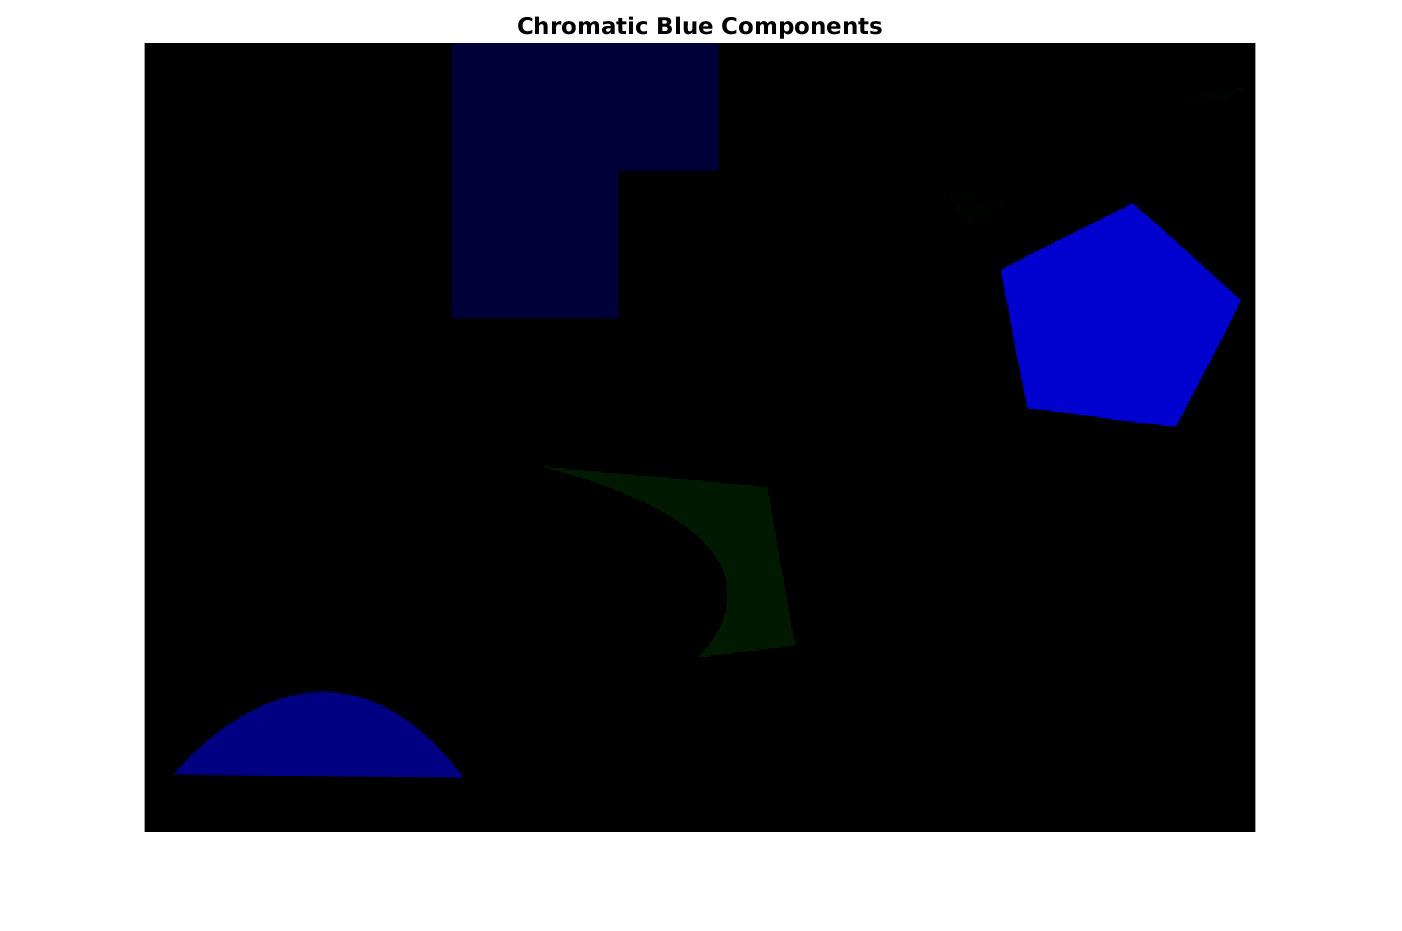
\includegraphics[width=\linewidth]{images/task2/drawingcb.png}
  \caption{Chromatic Blue component of Figure \ref{fig:drawing}.}
  \label{fig:drawingcb}
\end{figure}

\begin{figure}[h]
  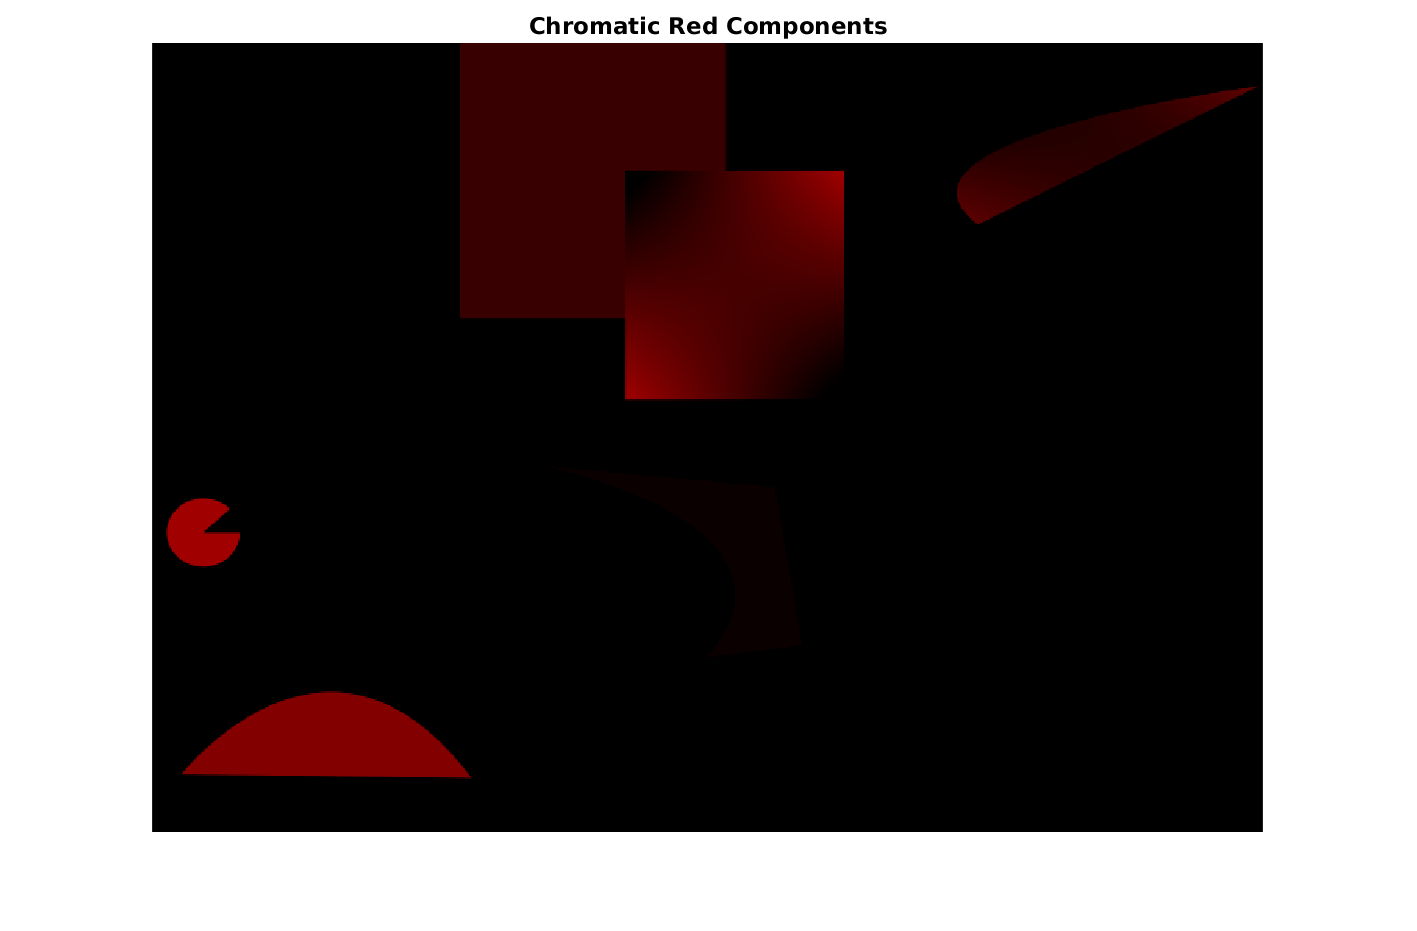
\includegraphics[width=\linewidth]{images/task2/drawingcr.png}
  \caption{Chromatic Red component of Figure \ref{fig:drawing}.}
  \label{fig:drawingcr}
\end{figure}

\begin{figure}[h]
  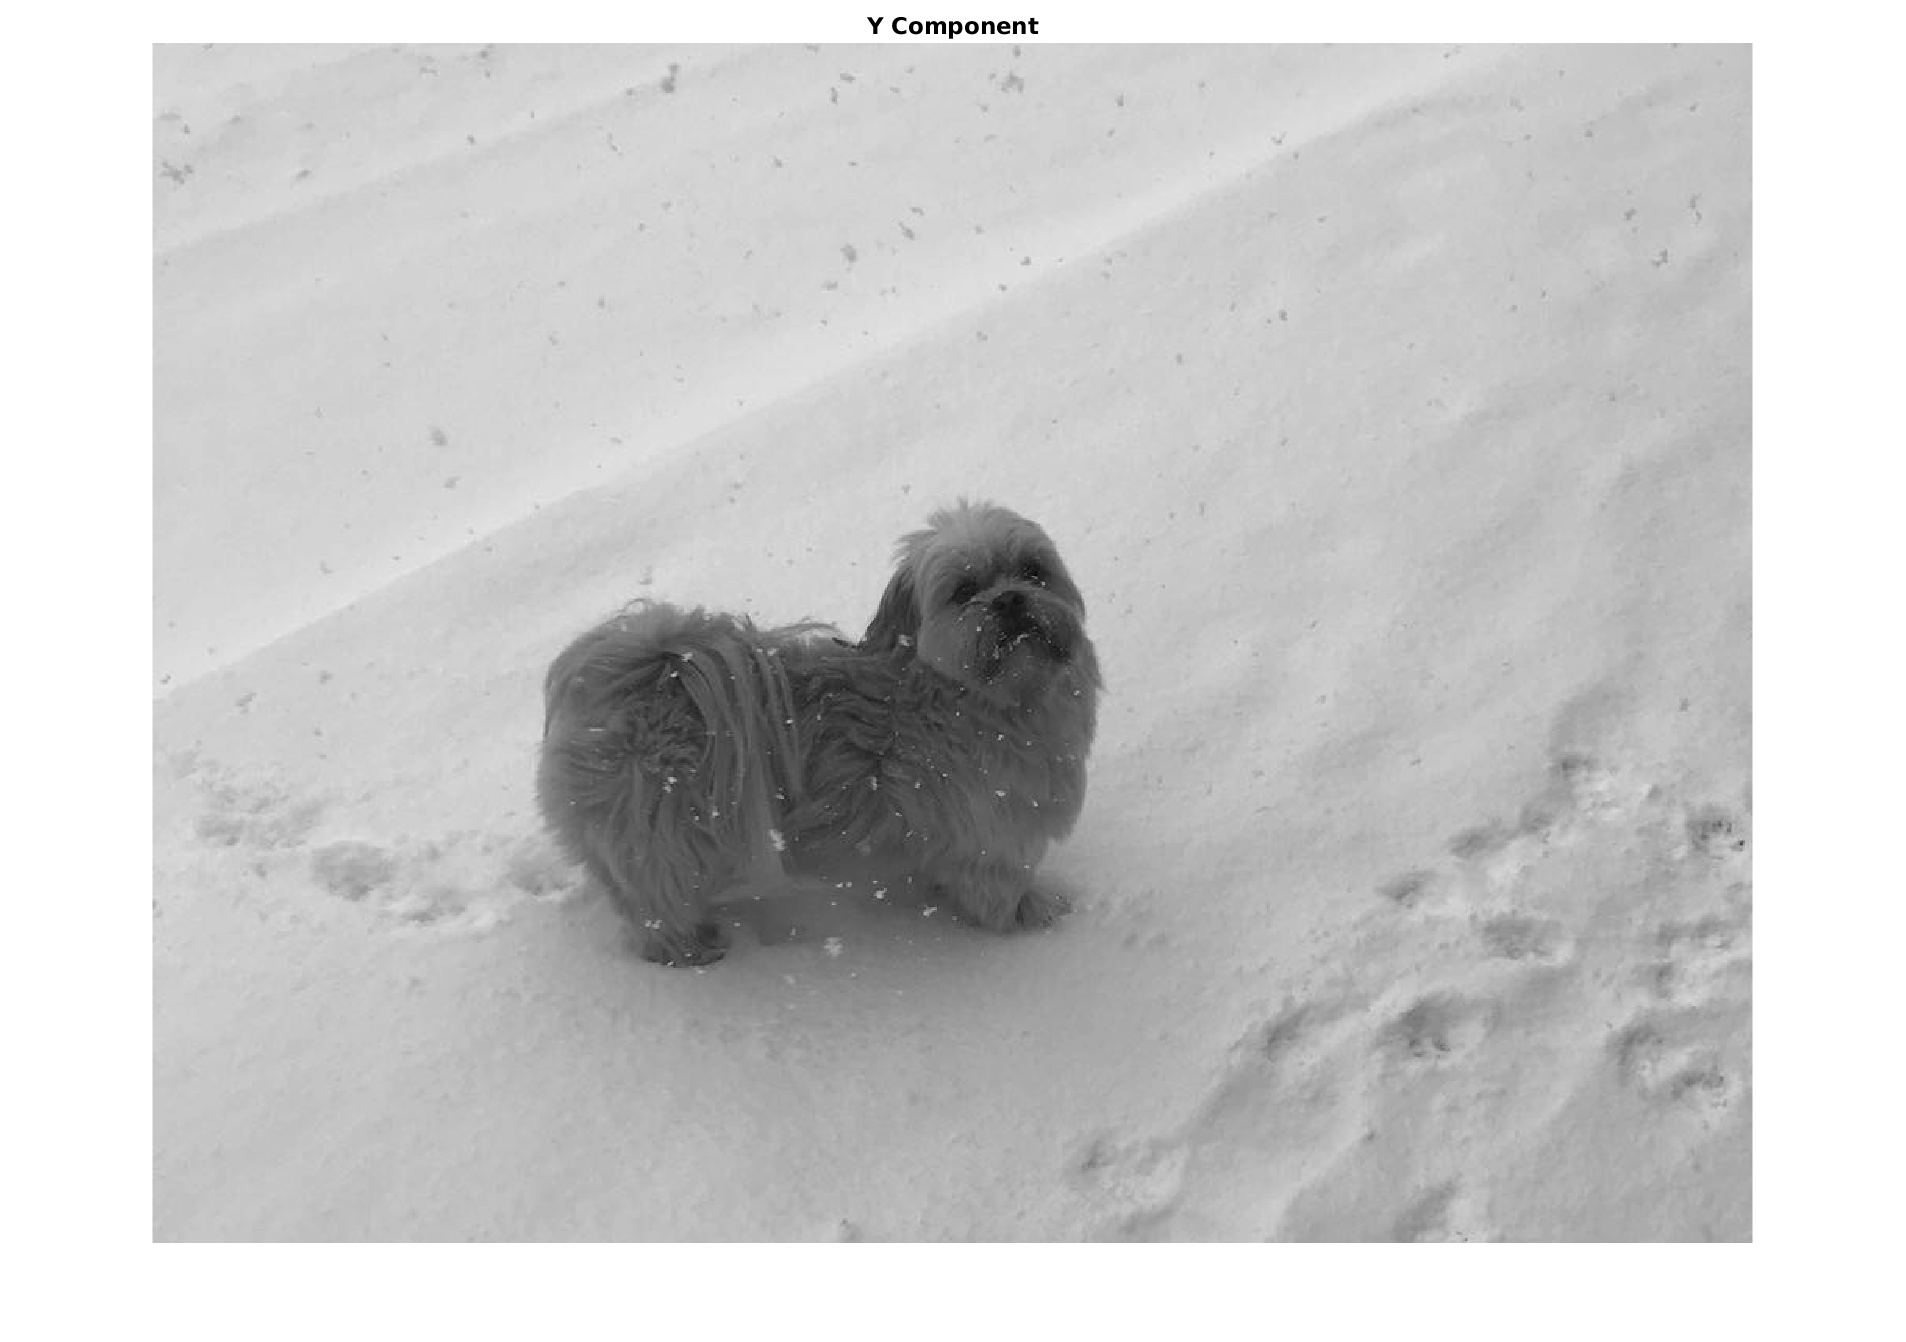
\includegraphics[width=\linewidth]{images/task2/simpley.png}
  \caption{Luminance component of Figure \ref{fig:simple}.}
  \label{fig:simpley}
\end{figure}

\begin{figure}[h]
  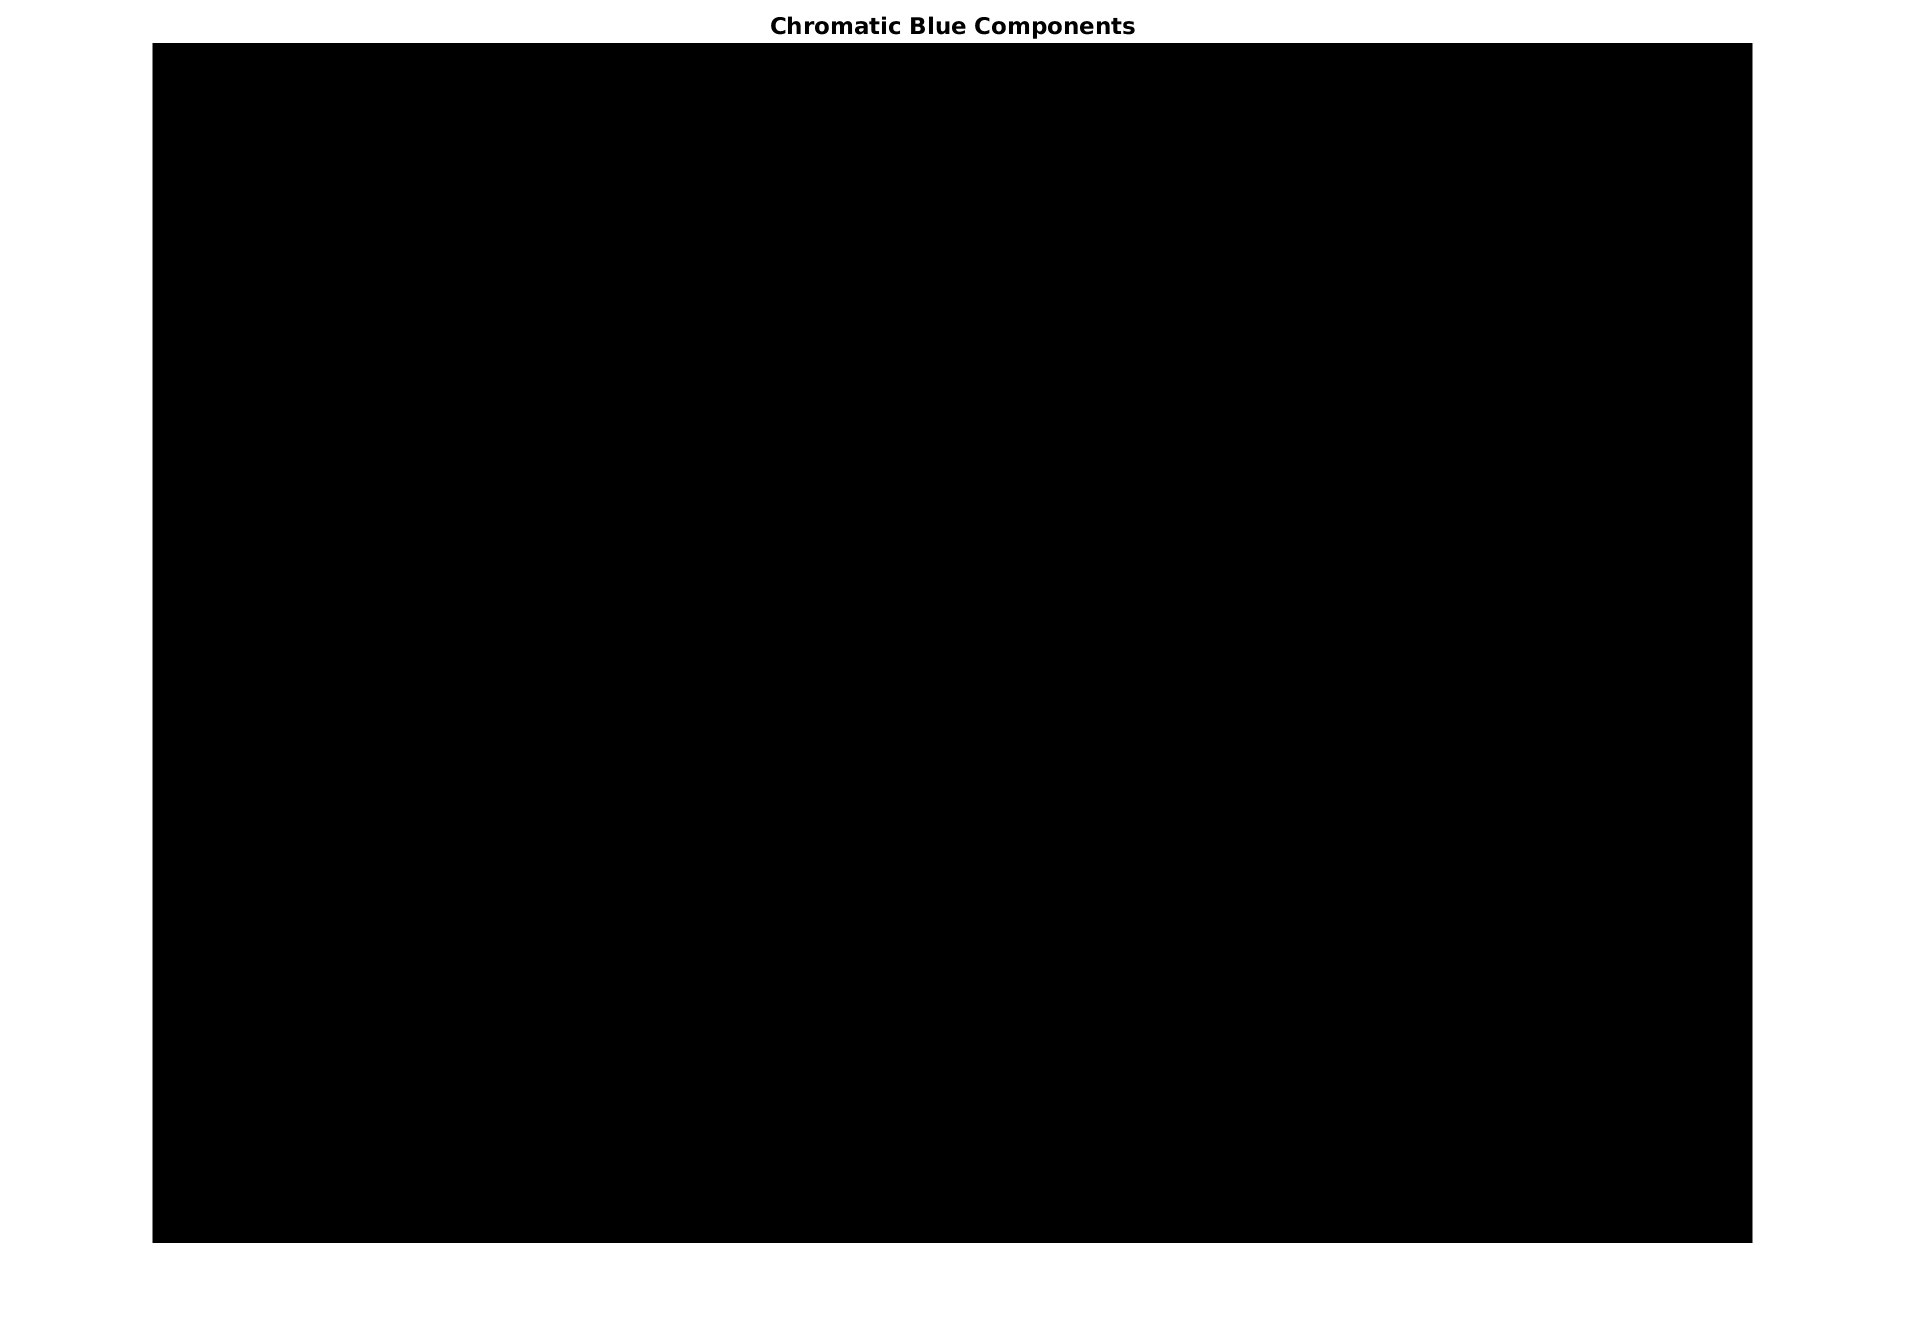
\includegraphics[width=\linewidth]{images/task2/simplecb.png}
  \caption{Chromatic Blue component of Figure \ref{fig:simple}.}
  \label{fig:simplecb}
\end{figure}

\begin{figure}[h]
  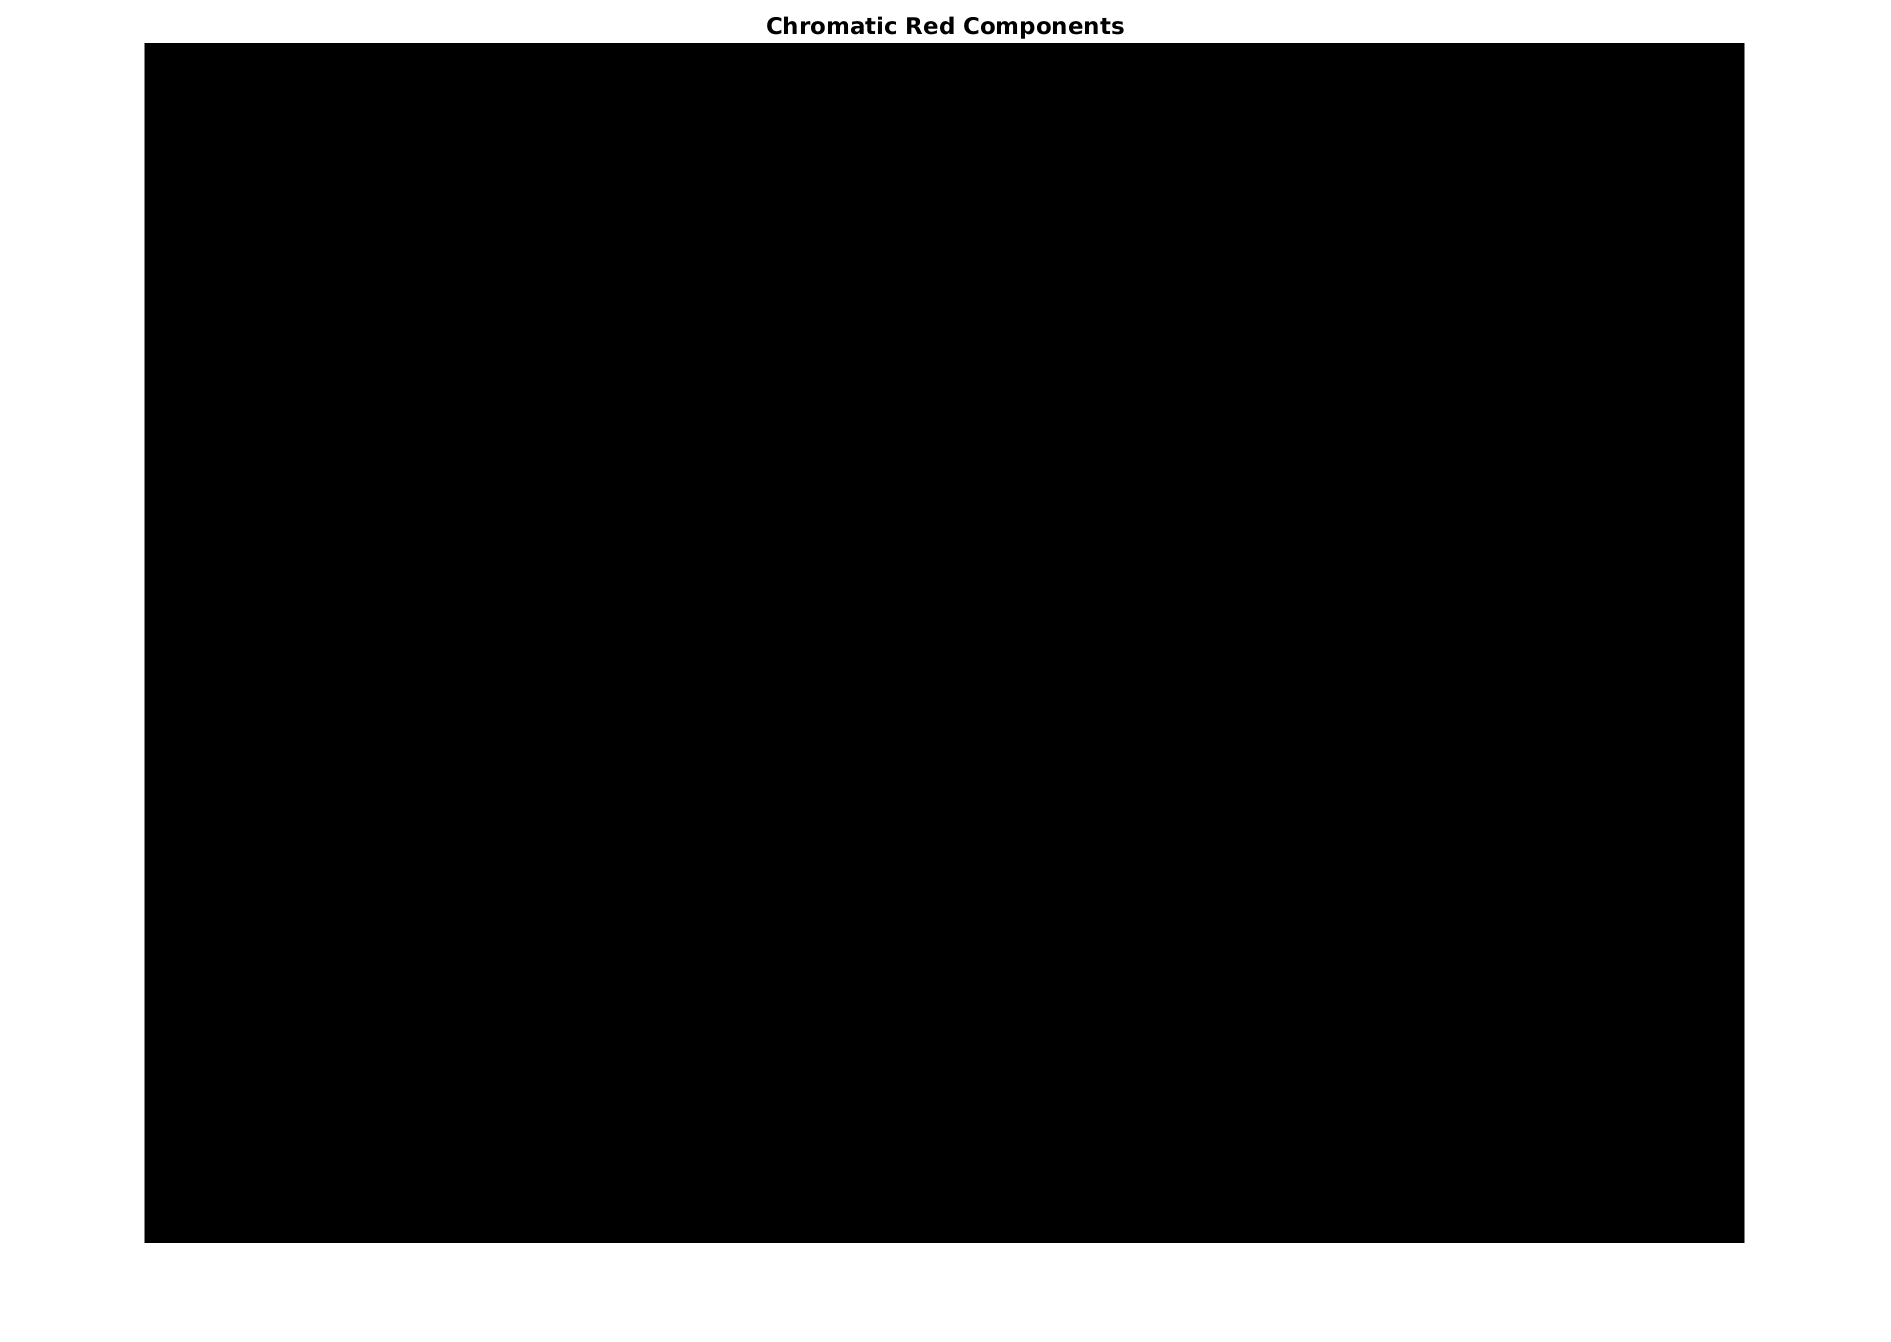
\includegraphics[width=\linewidth]{images/task2/simplecr.png}
  \caption{Chromatic Red component of Figure \ref{fig:simple}.}
  \label{fig:simplecr}
\end{figure}

\section{Downsampling}

This task required reducing the number of chroma samples by 8 in both dimensions of an image. This is often used in compression to reduce the amount of information being sent, as the human eye is more sensitive to changes in luminance (the y value) than changes in colour (Cb and Cr). To do this, the following operations were carried out:

\begin{enumerate}
  \item Convert the RGB image matrix to YCbCr.
  \item Trim the image to the nearest multiple of 8 in both dimensions in all channels.
  \item Split the image matrix into 8x8 cells.
  \item In the Cb and Cr layers, replace every value in each cell with the average of that cell.
  \item Concatenate the Y, Cb, and Cr matrices to produce the downsampled image.
\end{enumerate}

The values in each cell are replaced with the average to allow the image to be correctly rendered, but in transmission only one value per cell would need to be sent from the Cb and Cr channels. 

The results are shown in figures \ref{fig:colorfulsub} to \ref{fig:simplediff}. Each resulting subsampled YCbCr image appears to have pink and green hues. Since these exist at the extremes of the YCbCr range of colours, it's likely these are due to incorrect conversions to RGB. Ignoring this, it is still possible to see the effects of subsampling.

In the subsampled images of figure \ref{fig:colorful}, the macroblocks are fairly visible along the edges of objects. Thin outlines of objects that existed in the middle of a cell are thickened due to the averaging of the cells. It is harder to notice shapes in the chromatic images as outlines are less well defined. The cell blocks are especially apparent when the difference between the original and subsampled image are shown (Figure \ref{colorfulsub}). On the other hand, the blue lantern at the bottom right with the pattern of circles does not appear to suffer from aliasing.

\begin{figure}[h]
  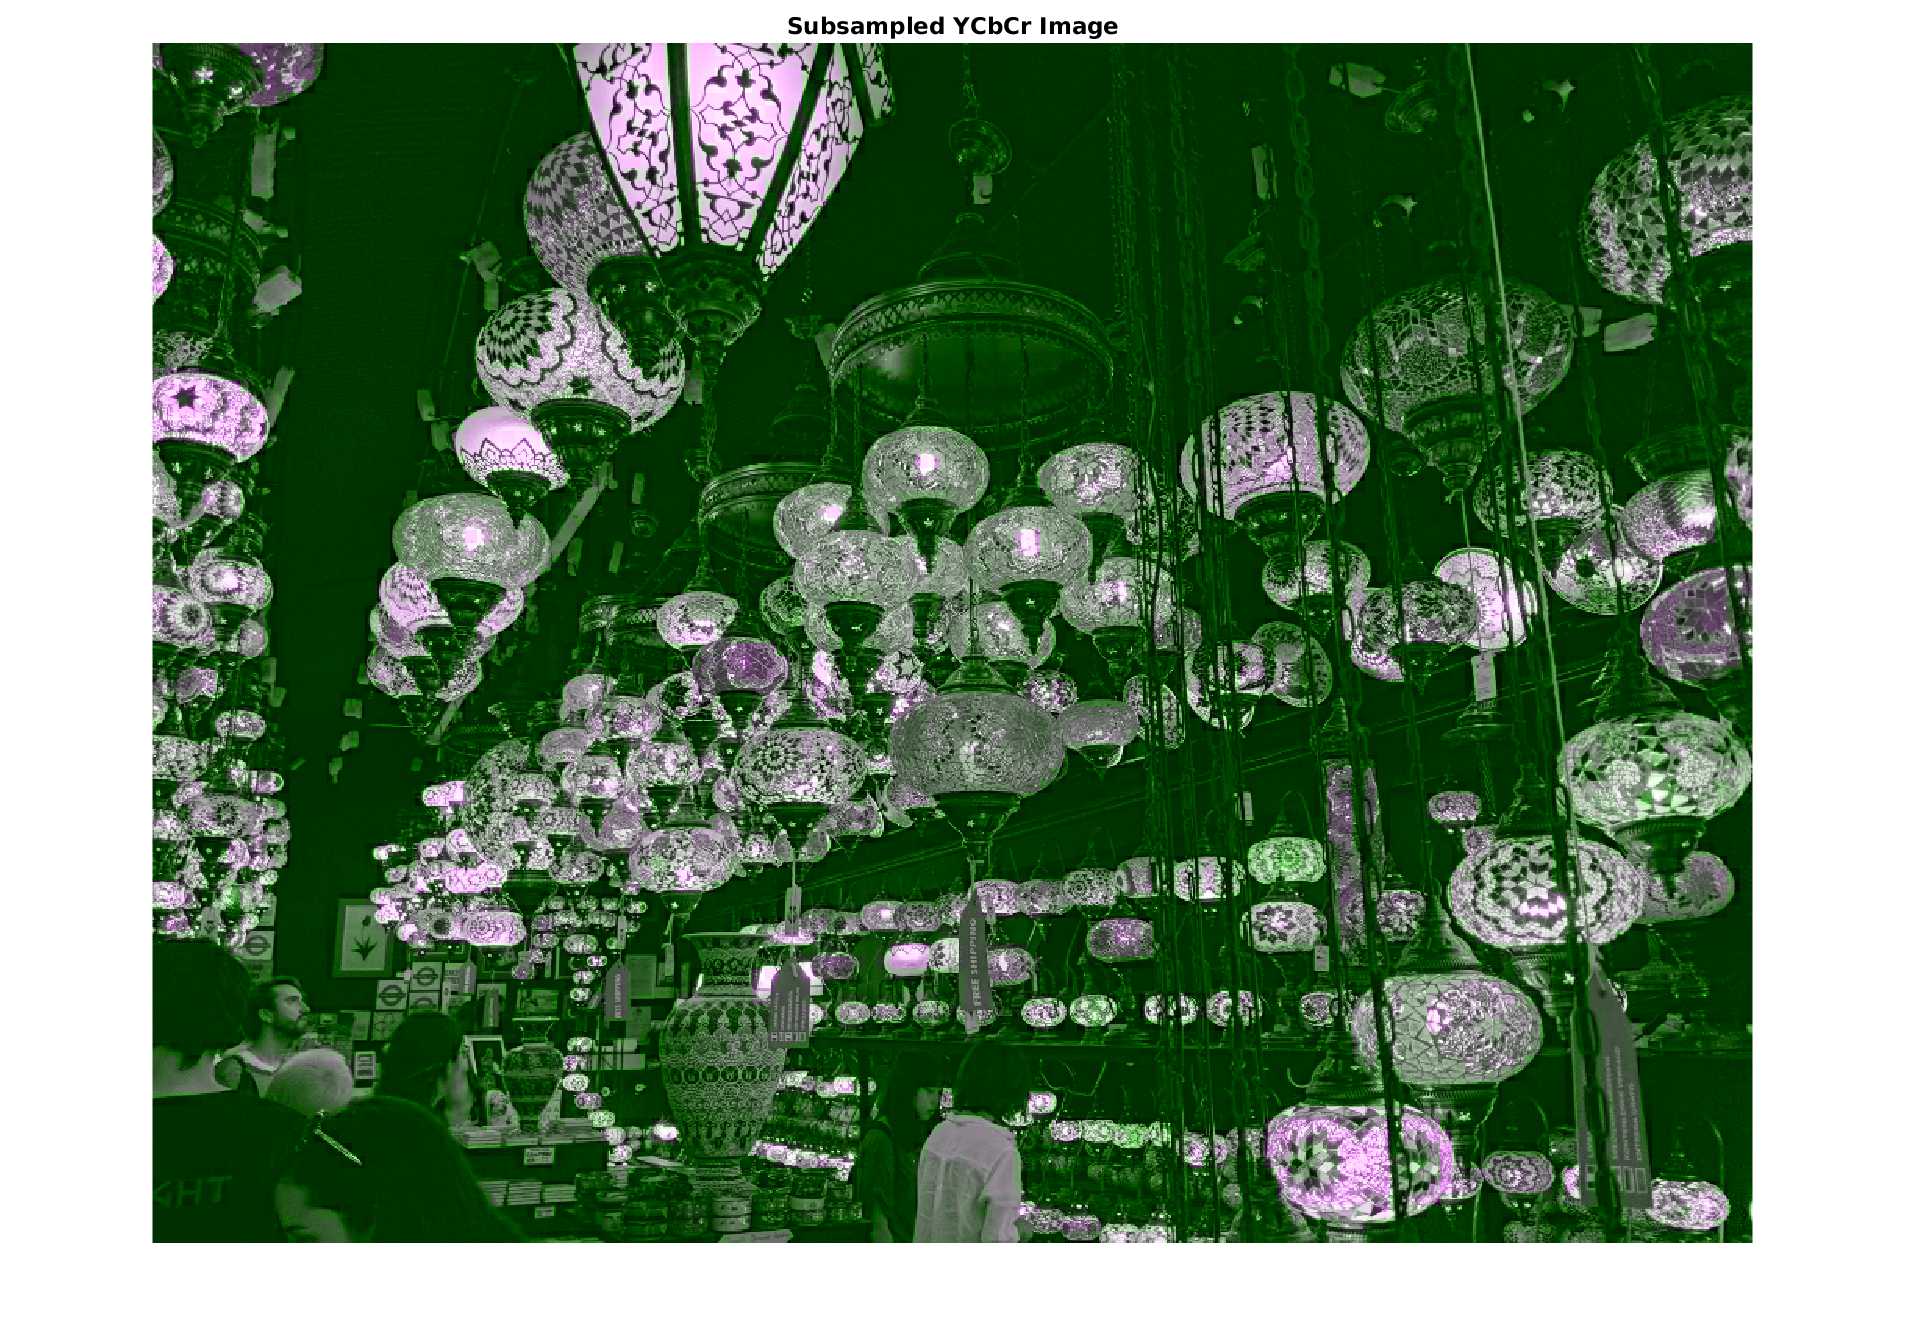
\includegraphics[width=\linewidth]{images/task3/colourfulsub.png}
  \caption{Subsampled version of Figure \ref{fig:colorful}.}
  \label{fig:colourfulsub}
\end{figure}

\begin{figure}[h]
  
\includegraphics[width=\linewidth]{images/task3/colourfuly.png}
  \caption{Luminance component of Figure \ref{fig:colorful}.}
  \label{fig:colourfulsuby}
\end{figure}

\begin{figure}[h]
  
\includegraphics[width=\linewidth]{images/task3/colourfulcb.png}
  \caption{Chromatic Blue component of Figure \ref{fig:colorful}.}
  \label{fig:colourfulsubcb}
\end{figure}

\begin{figure}[h]
  
\includegraphics[width=\linewidth]{images/task3/colourfulcr.png}
  \caption{Chromatic Red component of Figure \ref{fig:colorful}.}
  \label{fig:colourfulsubcr}
\end{figure}

\begin{figure}[h]
  \includegraphics[width=\linewidth]{images/task3/colourfulff.png}
  \caption{Difference between Figure \ref{fig:colorful} and Figure \ref{fig:colorfulsub}.}
  \label{fig:colourfuldiff}
\end{figure}

In the subsampled image of the drawing, the effect of aliasing is far more apparent. The thin edges of objects have harsh muddy outlines due to the average of the two colours. 

\begin{figure}[h]
  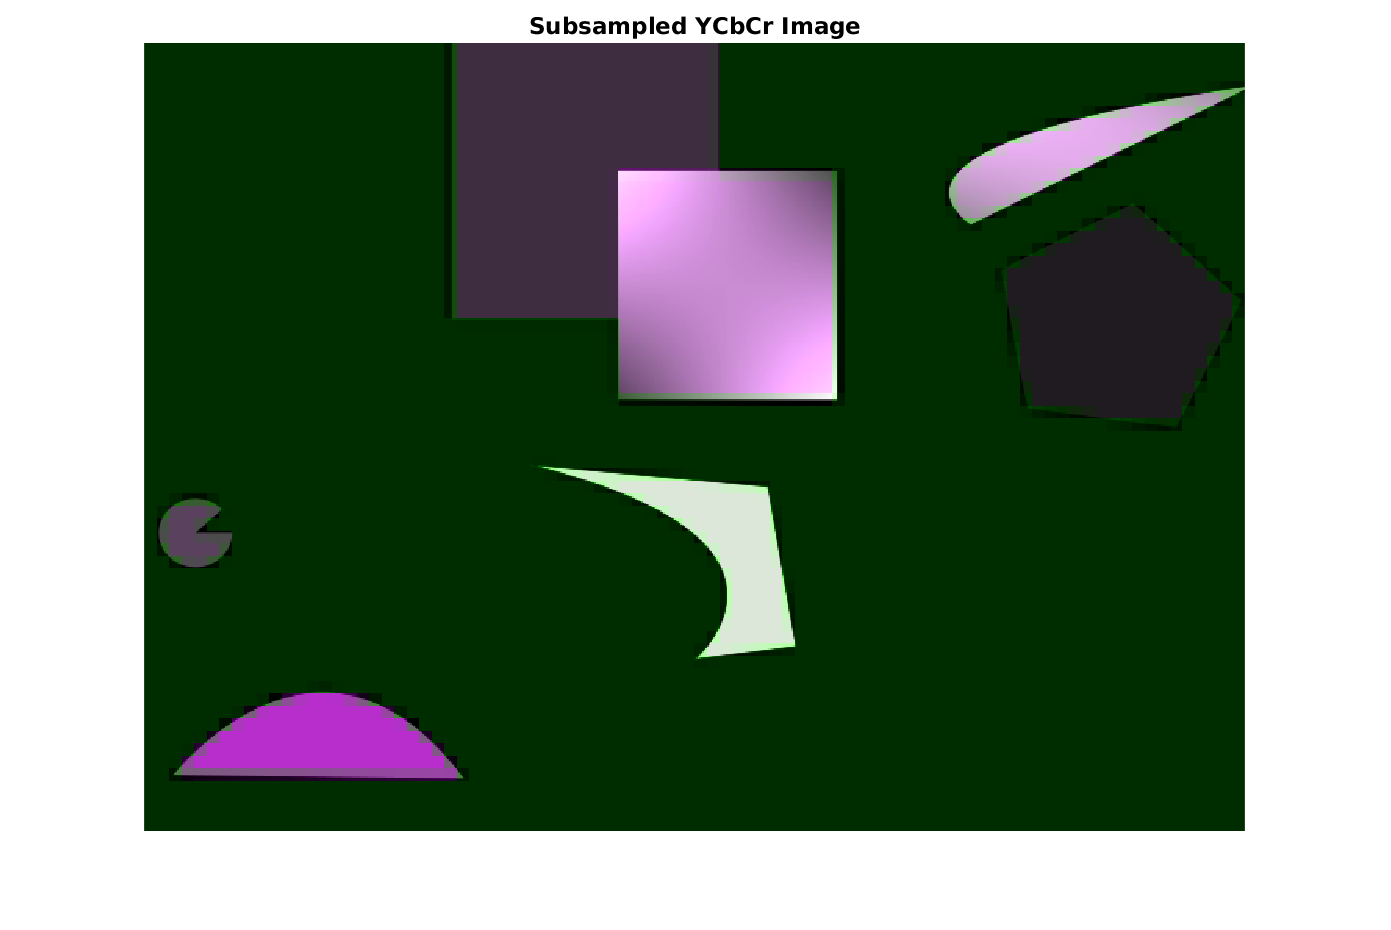
\includegraphics[width=\linewidth]{images/task3/drawingsub.png}
  \caption{Subsampled version of Figure \ref{fig:drawing}.}
  \label{fig:drawingsub}
\end{figure}

\begin{figure}[h]
  
\includegraphics[width=\linewidth]{images/task3/drawingy.png}
  \caption{Luminance component of Figure \ref{fig:drawing}.}
  \label{fig:drawingsuby}
\end{figure}

\begin{figure}[h]
  
\includegraphics[width=\linewidth]{images/task3/drawingcb.png}
  \caption{Chromatic Blue component of Figure \ref{fig:drawing}.}
  \label{fig:drawingsubcb}
\end{figure}

\begin{figure}[h]
  
\includegraphics[width=\linewidth]{images/task3/drawingcr.png}
  \caption{Chromatic Red component of Figure \ref{fig:drawing}.}
  \label{fig:drawingsubcr}
\end{figure}

\begin{figure}[h]
  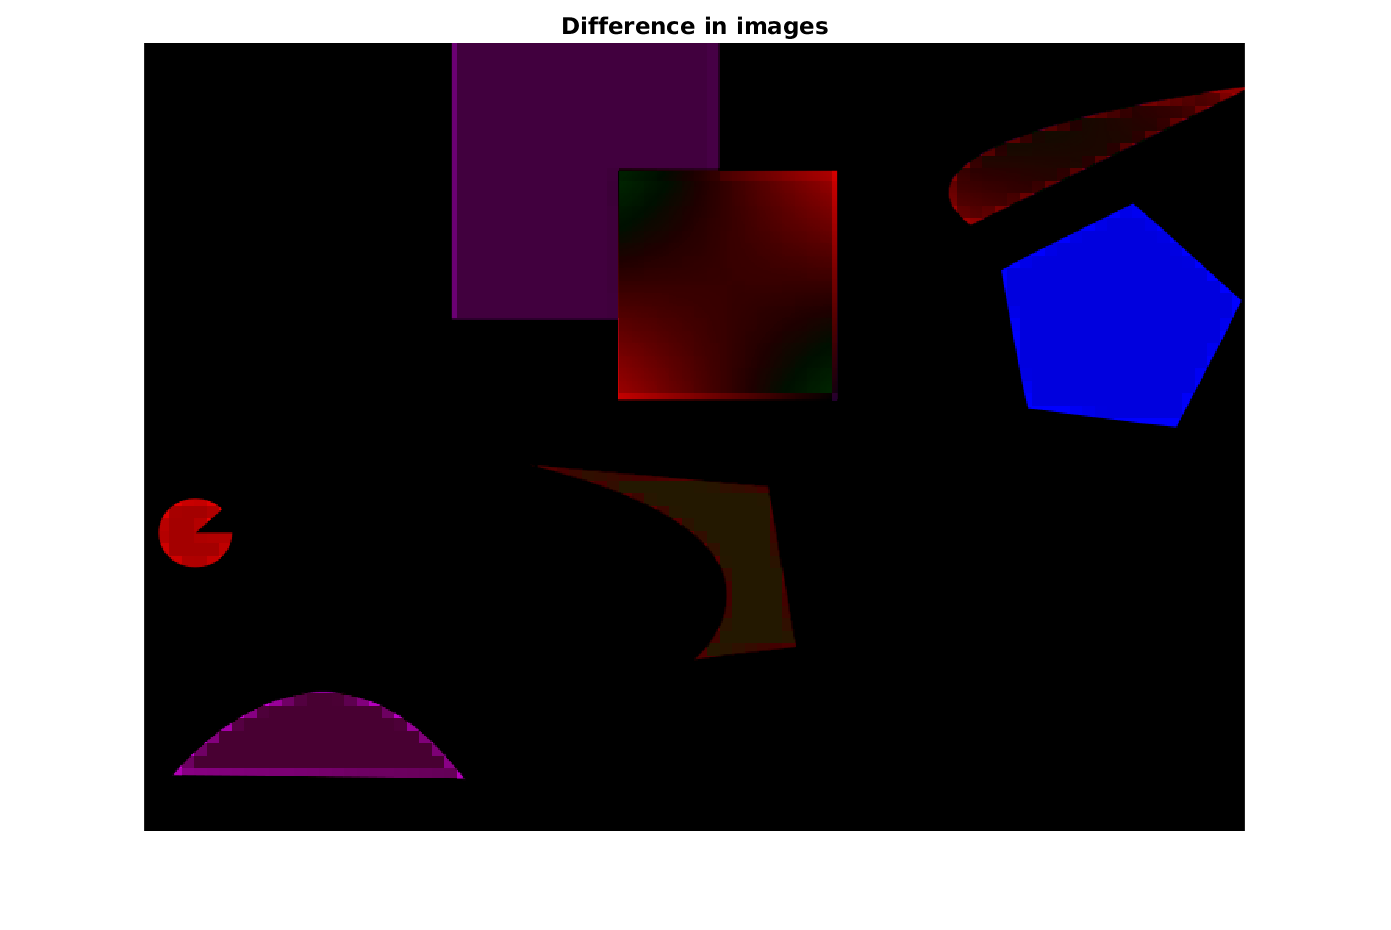
\includegraphics[width=\linewidth]{images/task3/drawingdiff.png}
  \caption{Difference between Figure \ref{fig:drawing} and Figure \ref{fig:drawingsub}.}
  \label{fig:drawingdiff}
\end{figure}

The simple image was the least affected by downsampling. Since the Cb and Cr values were basically both ~128, the fine grained details remained, for example, the dogs fur or the falling snow. At the edges of the dog where a sudden contrast in luminance occurs, some aliasing can be seen.

\begin{figure}[h]
  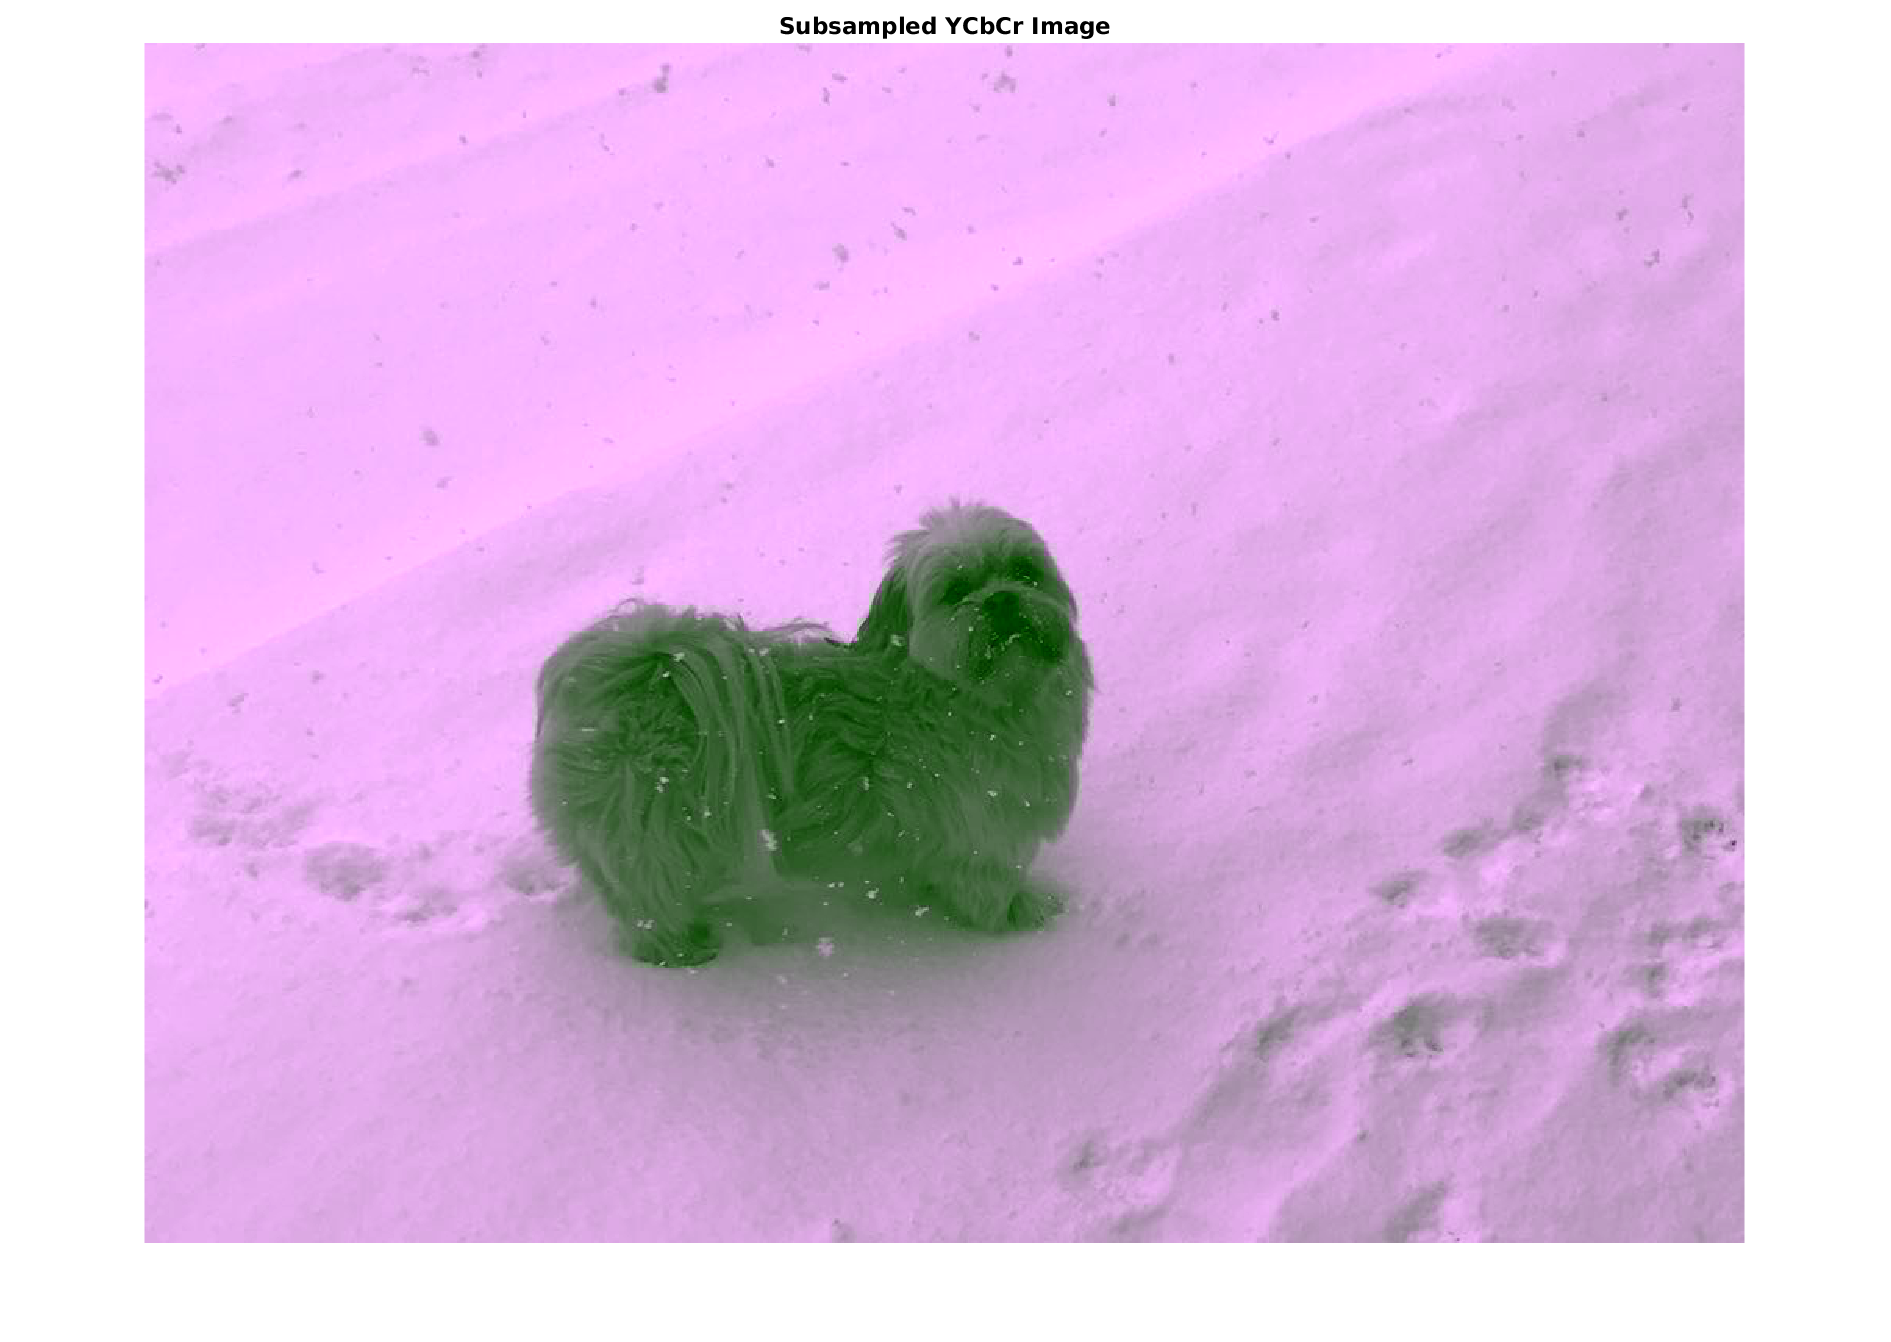
\includegraphics[width=\linewidth]{images/task3/simplesub.png}
  \caption{Subsampled version of Figure \ref{fig:simple}.}
  \label{fig:simplesub}
\end{figure}

\begin{figure}[h]
  
\includegraphics[width=\linewidth]{images/task3/simpley.png}
  \caption{Luminance component of Figure \ref{fig:simple}.}
  \label{fig:simplesuby}
\end{figure}

\begin{figure}[h]
  
\includegraphics[width=\linewidth]{images/task3/simplecb.png}
  \caption{Chromatic Blue component of Figure \ref{fig:simple}.}
  \label{fig:simplesubcb}
\end{figure}

\begin{figure}[h]
  
\includegraphics[width=\linewidth]{images/task3/simplecr.png}
  \caption{Chromatic Red component of Figure \ref{fig:simple}.}
  \label{fig:simplesubcr}
\end{figure}

\begin{figure}[h]
  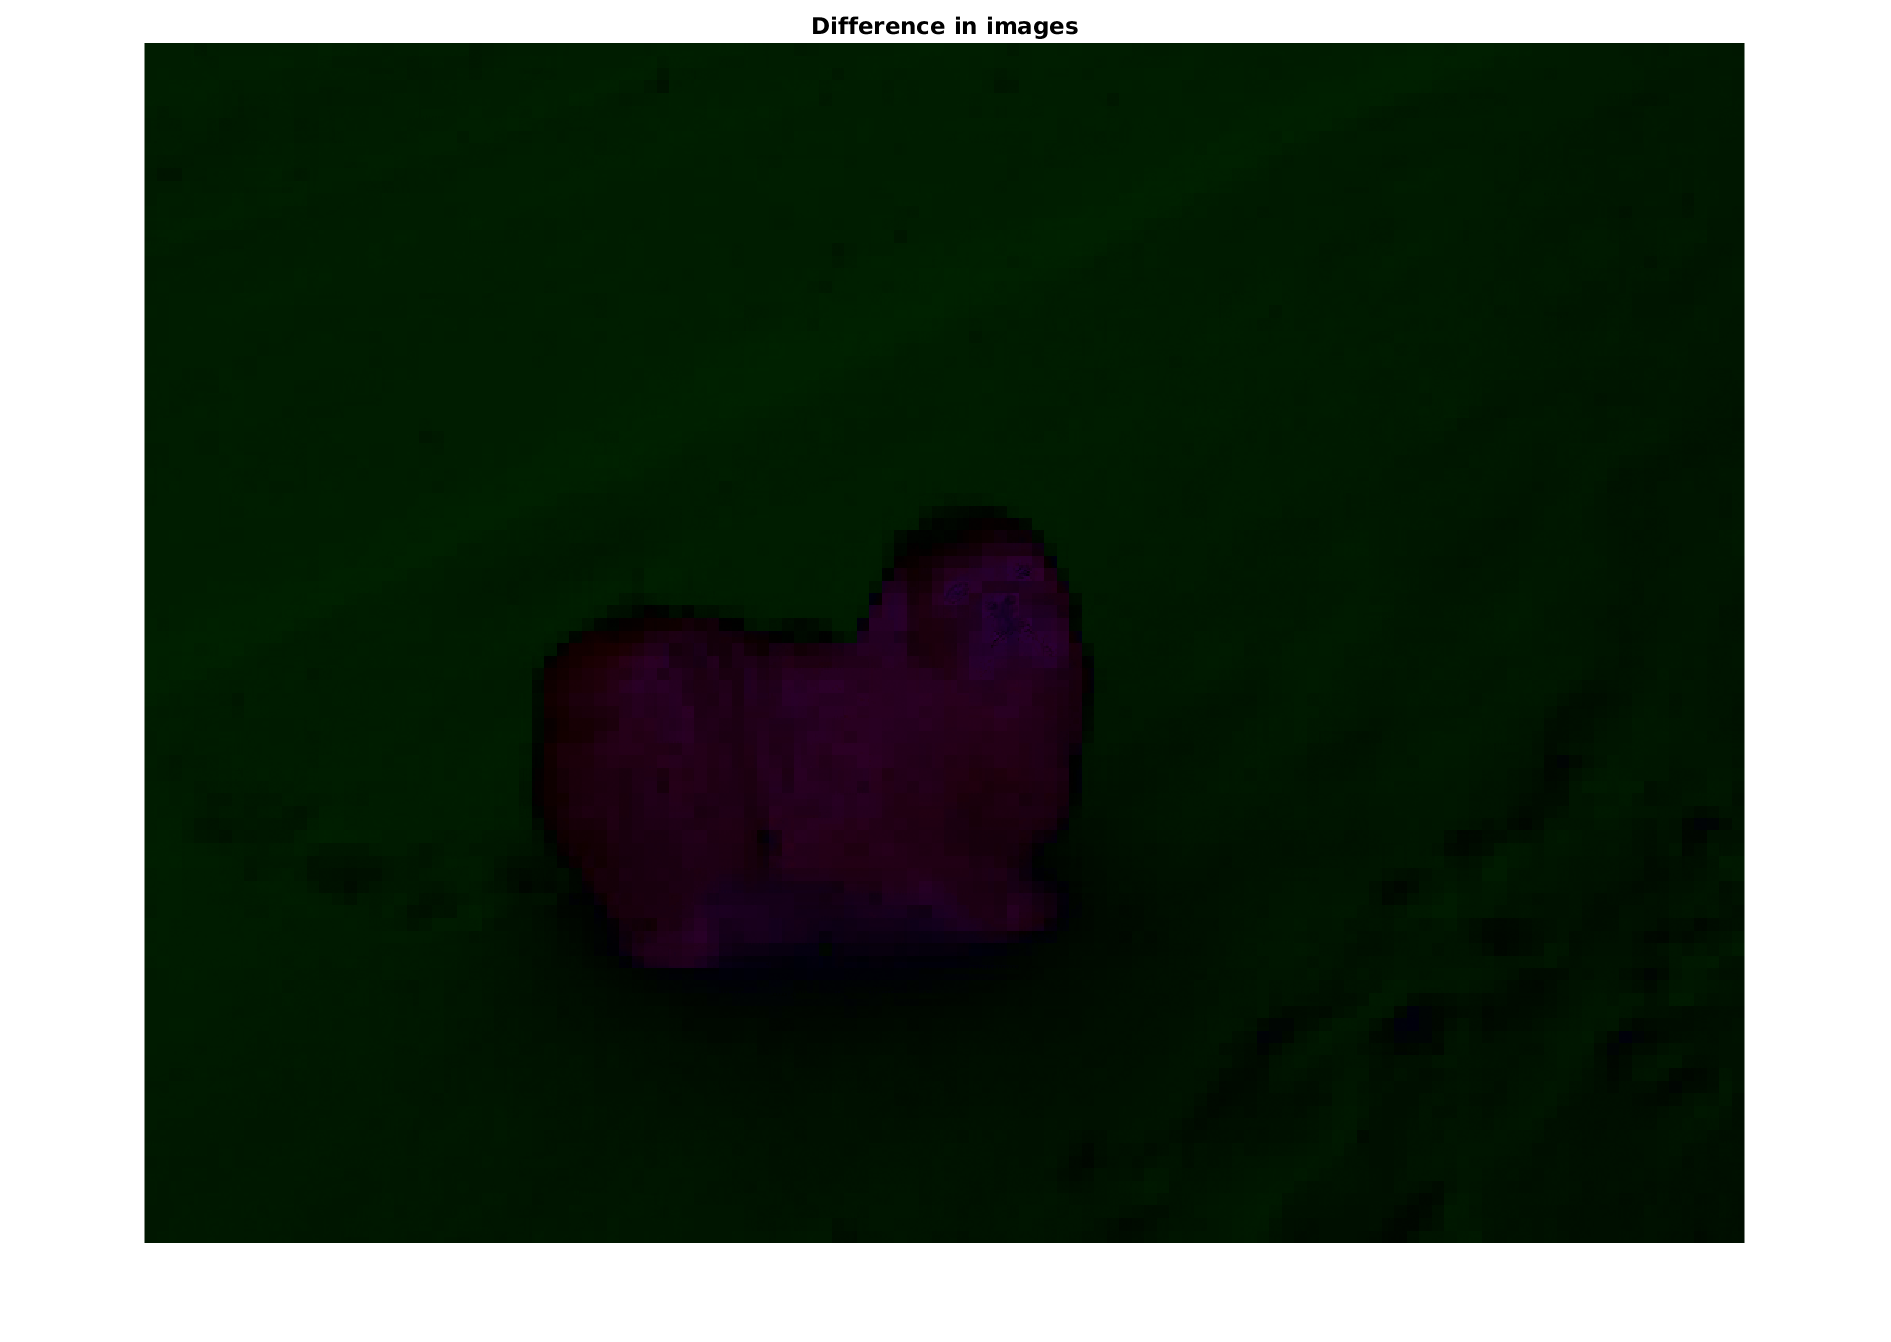
\includegraphics[width=\linewidth]{images/task3/simplediff.png}
  \caption{Difference between Figure \ref{fig:simple} and Figure \ref{fig:simplesub}.}
  \label{fig:simplediff}
\end{figure}

\section{Discrete Cosine Transform}

The spatial frequency was plotted for each channel for each image seperately. Unfortunately I was unable to force colourbars to appear for the correct figures, and so some plots do not have a colorbar that should. The plots were produced by performing the 2D discrete cosine transform (\emph{dct2} function in Matlab) on each channel matrix. For plotting, the log of the absolute value of the results taken. In reality, the DCT is used applied to 8x8 pixel cells at a time, and memoisation is used instead of computation to produce the result. Though the DCT and FFT both provide frequencies, DCTs are able to produce straight lines using fewer coefficients, making it slightly more memory efficient. 

For the DCT of figure \ref{fig:colorful}, each channel shows a large spread of spatial frequencies (Given the large amount of white even at the bottom-right corner of the figure). This is expected, as the image features constant changes in colour, straight and curved lines of varying lengths, and lots of different patterns. As an extension, the low and high frequency components were also isolated. In JPEG compression, the high frequency components would be removed using a similar approach. The plot of the low frequency image shows very little, likely due to the large amount of detail present in the image (though it is suspiciously too little detail, and may be due to error). On the other hand, the high spatial frequency plot contains enough detail to notice details from the orignal image.

\begin{figure}[h]
  
\includegraphics[width=\linewidth]{images/task4/colourfuly.png}
  \caption{Spatial frequencies of Y Component of Figure \ref{fig:colorful}.}
  \label{fig:colorfulyspatial}
\end{figure}

\begin{figure}[h]
  
\includegraphics[width=\linewidth]{images/task4/colourfulcb.png}
  \caption{Spatial frequencies of Cb Component of Figure \ref{fig:colorful}.}
  \label{fig:colorfulcbspatial}
\end{figure}

\begin{figure}[h]
  
\includegraphics[width=\linewidth]{images/task4/colourfulcr.png}
  \caption{Spatial frequencies of Cr Component of Figure \ref{fig:colorful}.}
  \label{fig:colorfulcrspatial}
\end{figure}

\begin{figure}[h]
  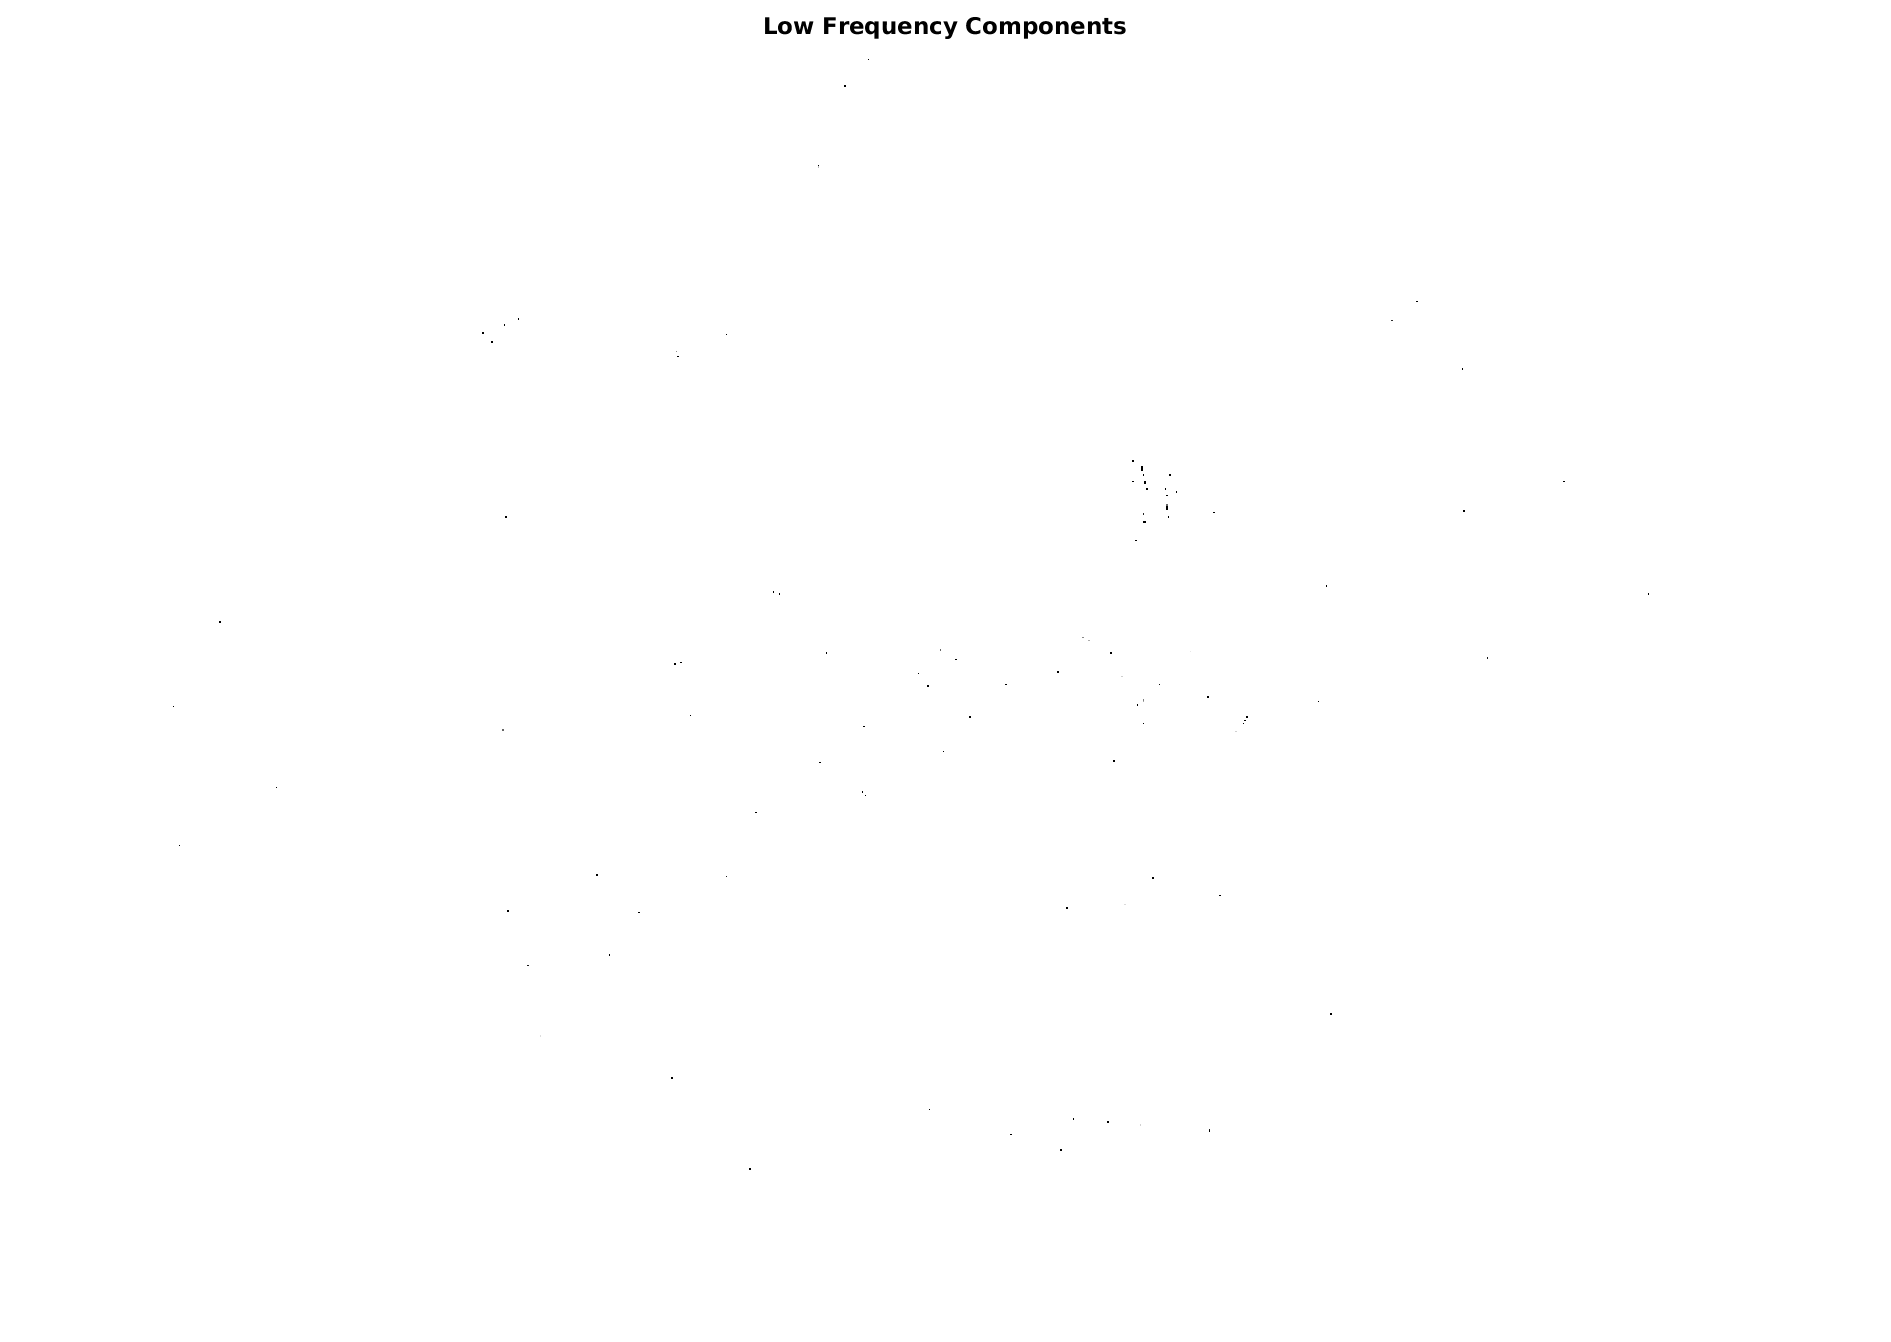
\includegraphics[width=\linewidth]{images/task4/colourfullf.png}
  \caption{Low spatial frequencies of Y Component of Figure \ref{fig:colorful}.}
  \label{fig:colorfulylfspatial}
\end{figure}

\begin{figure}[h]
  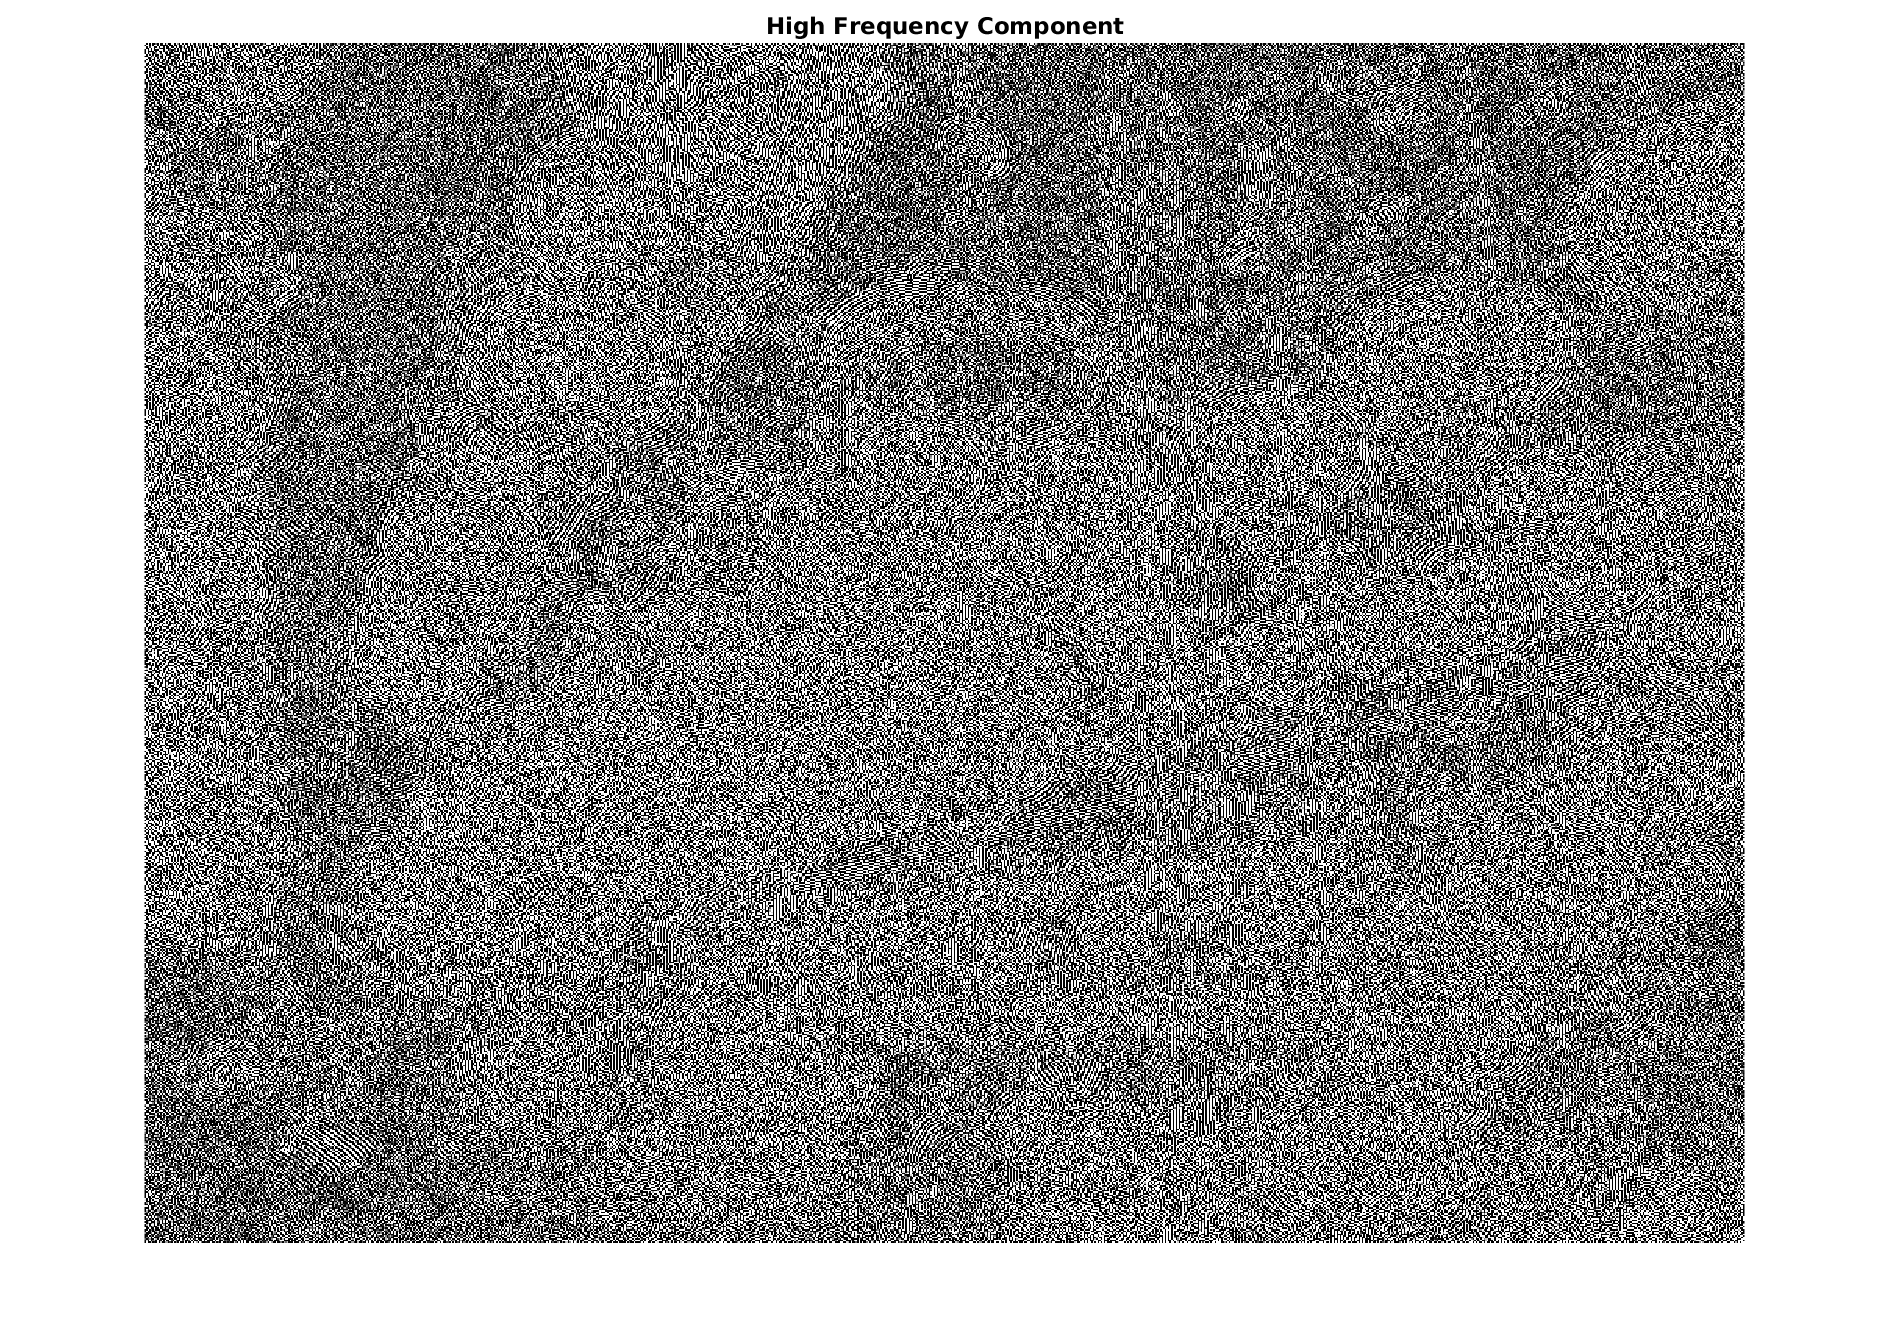
\includegraphics[width=\linewidth]{images/task4/colourfulhf.png}
  \caption{High spatial frequencies of Y Component of Figure \ref{fig:colorful}.}
  \label{fig:colorfulylfspatial}
\end{figure}

The DCT plots of the vector image show more focused frequencies. Most of the energy is focused in the top left, corresponding to low spatial frequency components. This is likely due to the abundance of long lines and no textures. The large triangle that is present in the DCT of all three channels is likely responsible for producing the curved lines in the image, as it would require a gradual change in the coeffiecients used to move the maxima responsible for generating the line.

The plot of the high frequency components supports this, as the curves are very clear in the highpass filtered image.  

\begin{figure}[h]
  
\includegraphics[width=\linewidth]{images/task4/drawingy.png}
  \caption{Spatial frequencies of Y Component of Figure \ref{fig:drawing}.}
  \label{fig:drawingyspatial}
\end{figure}

\begin{figure}[h]
  
\includegraphics[width=\linewidth]{images/task4/drawingcb.png}
  \caption{Spatial frequencies of Cb Component of Figure \ref{fig:drawing}.}
  \label{fig:drawingcbspatial}
\end{figure}

\begin{figure}[h]
  
\includegraphics[width=\linewidth]{images/task4/drawingcr.png}
  \caption{Spatial frequencies of Cr Component of Figure \ref{fig:drawing}.}
  \label{fig:drawingcrspatial}
\end{figure}

\begin{figure}[h]
  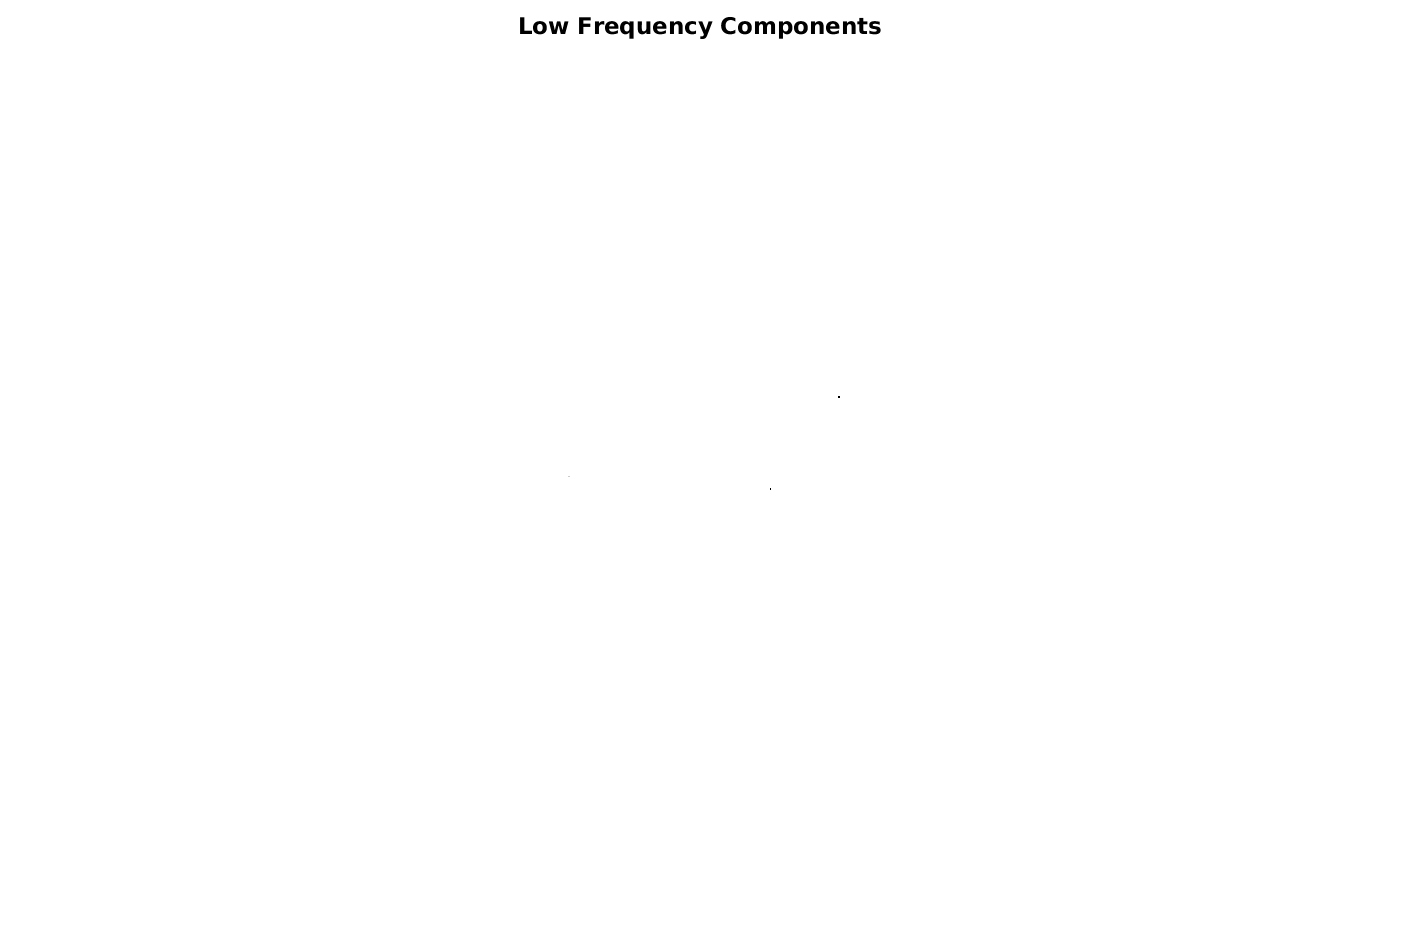
\includegraphics[width=\linewidth]{images/task4/drawinglf.png}
  \caption{Low spatial frequencies of Y Component of Figure \ref{fig:drawing}.}
  \label{fig:drawingylfspatial}
\end{figure}

\begin{figure}[h]
  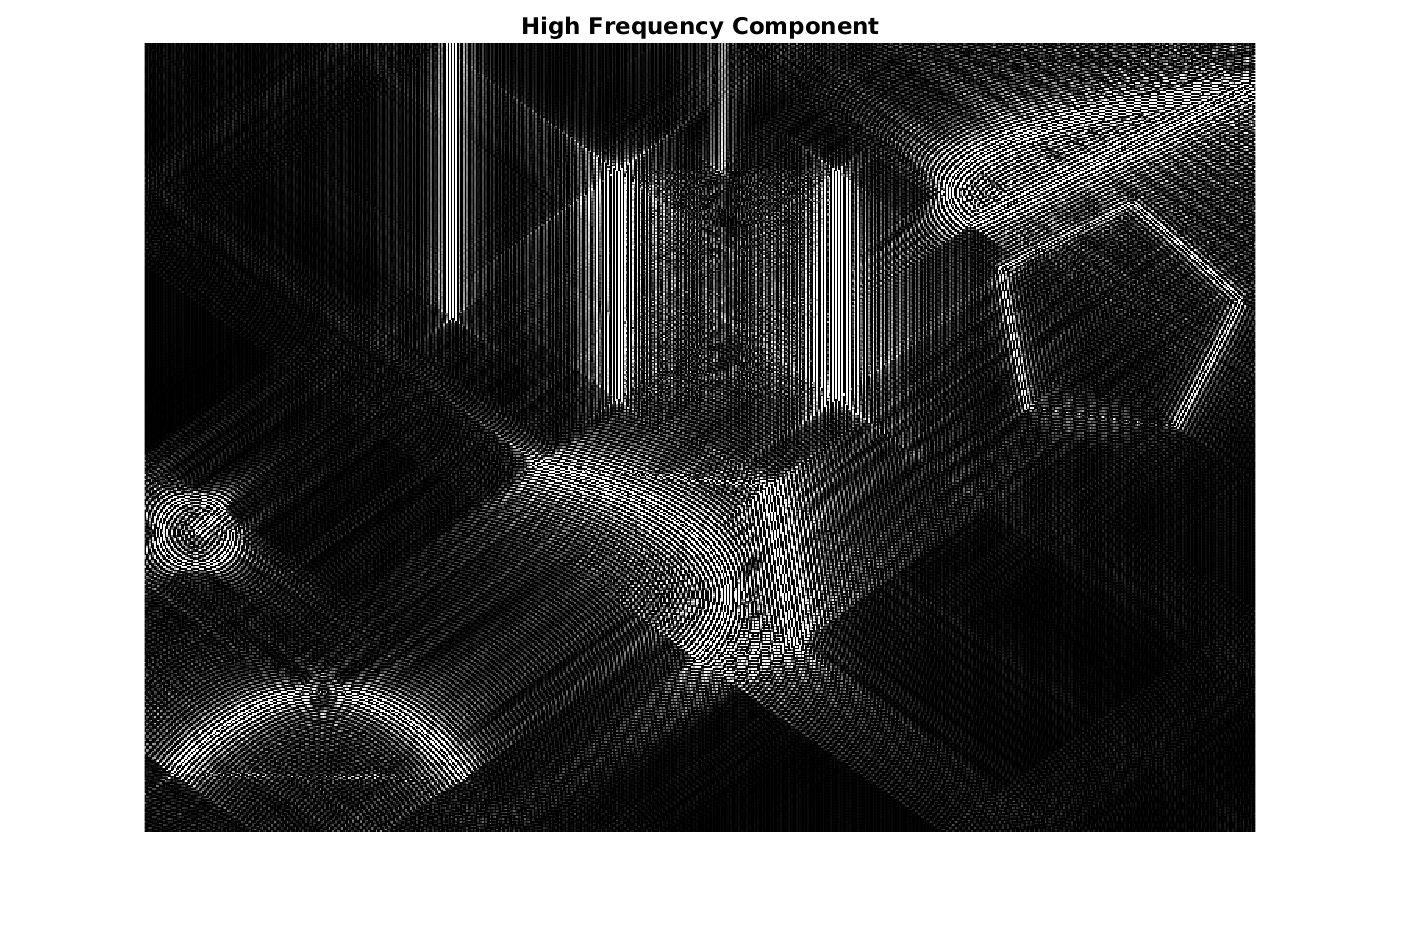
\includegraphics[width=\linewidth]{images/task4/drawinghf.png}
  \caption{High spatial frequencies of Y Component of Figure \ref{fig:drawing}.}
  \label{fig:drawingylfspatial}
\end{figure}

% Simple 

\begin{figure}[h]
  
\includegraphics[width=\linewidth]{images/task4/simpley.png}
  \caption{Spatial frequencies of Y Component of Figure \ref{fig:simple}.}
  \label{fig:simpleyspatial}
\end{figure}

\begin{figure}[h]
  
\includegraphics[width=\linewidth]{images/task4/simplecb.png}
  \caption{Spatial frequencies of Cb Component of Figure \ref{fig:simple}.}
  \label{fig:simplecbspatial}
\end{figure}

\begin{figure}[h]
  
\includegraphics[width=\linewidth]{images/task4/simplecr.png}
  \caption{Spatial frequencies of Cr Component of Figure \ref{fig:simple}.}
  \label{fig:simplecrspatial}
\end{figure}

\begin{figure}[h]
  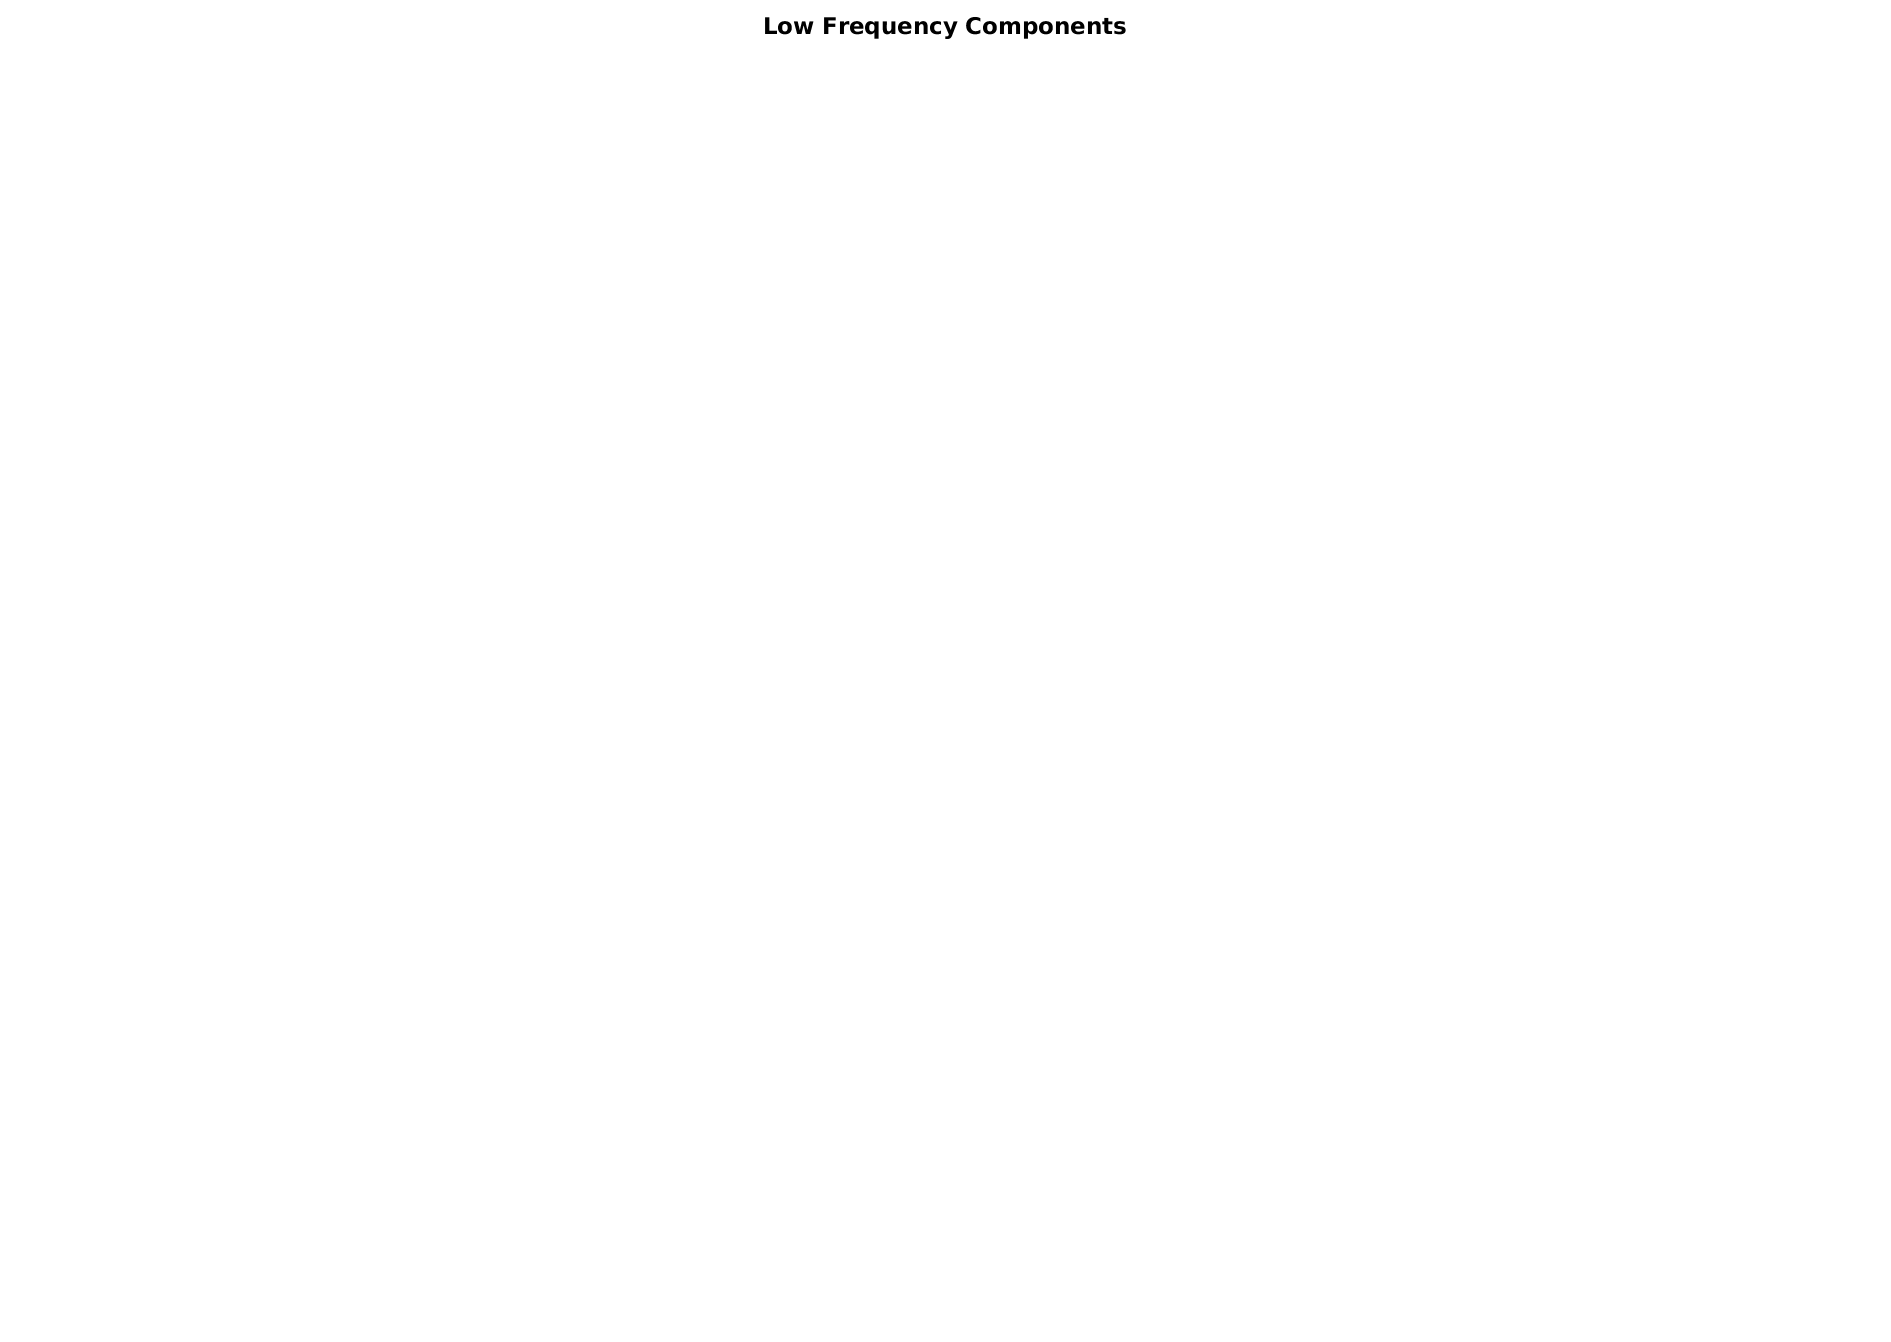
\includegraphics[width=\linewidth]{images/task4/simplelf.png}
  \caption{Low spatial frequencies of Y Component of Figure \ref{fig:simple}.}
  \label{fig:simpleylfspatial}
\end{figure}

\begin{figure}[h]
  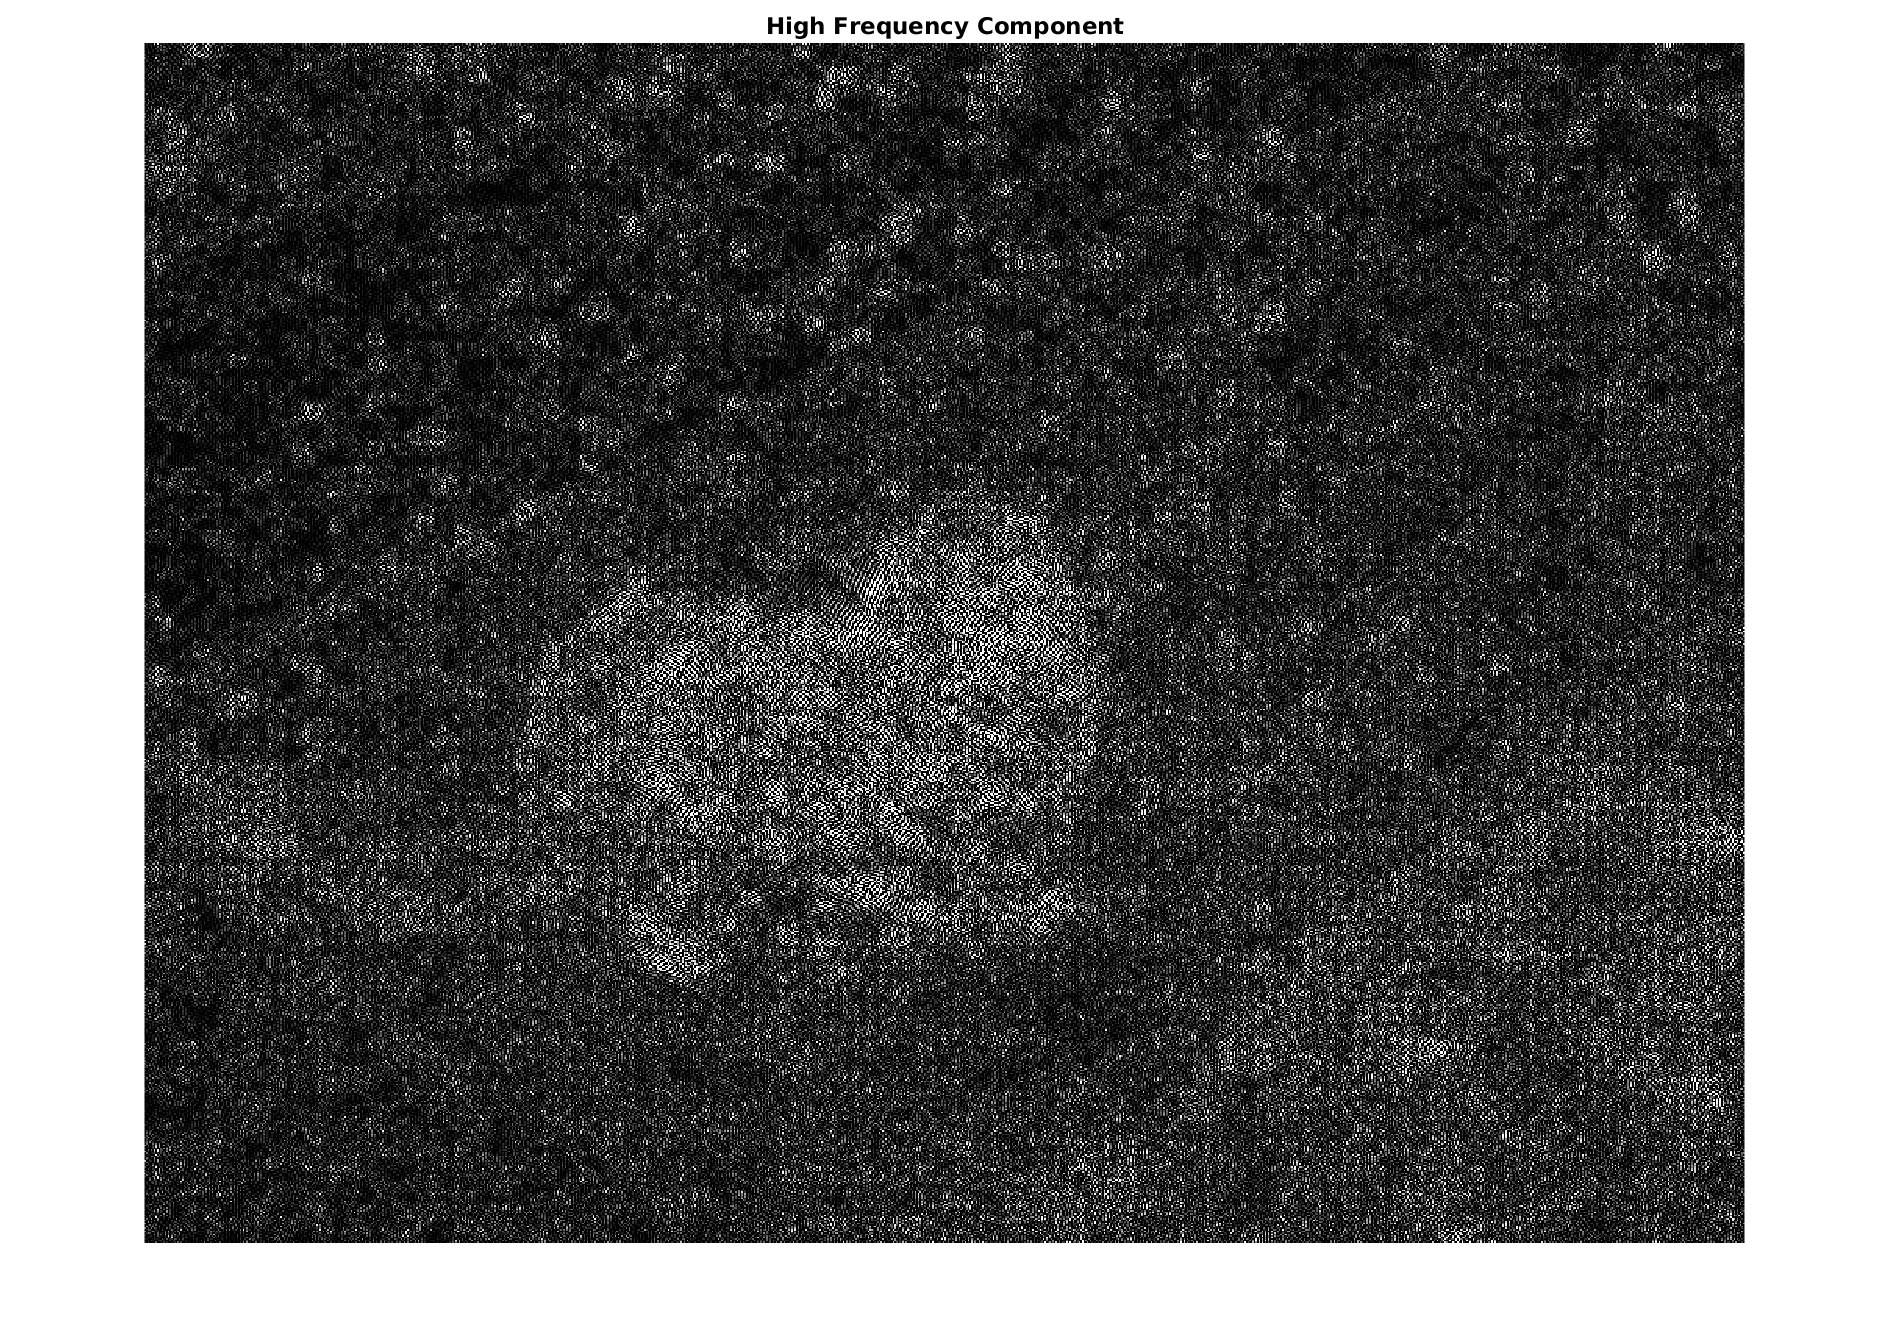
\includegraphics[width=\linewidth]{images/task4/simplehf.png}
  \caption{High spatial frequencies of Y Component of Figure \ref{fig:simple}.}
  \label{fig:simpleylfspatial}
\end{figure}

\part*{Conclusion}

This practical was incredibly enjoyable (excluding the whine), and greatly helped my understanding of Matlab. Actually implementing the technologies discussed in lectures resulted in many rabbit holes of learning, and a better understanding of the content. For example, the various types of audio filters and their pros and cons, and why it isn't as simple as 'blocking' the unwanted frequencies. 

I realised only close to the deadline that since on the schools Windows installs, the older version of Matlab (2017a) is used, and it did not have the bandpass function yet. However, in 2018b, it does exist, and so the scripts will only work on the linux machines. Given more time, I would have liked to replace the bandpass function with the more specific filters available, such as elliptical and chebyshev filters. 

\bibliographystyle{unsrt}
\bibliography{mybib}

\end{document}
